% !TEX encoding = UTF-8 Unicode
% !BIB TS-program = biber

% This file is MIT-Thesis.tex, a LaTeX template for formatting an MIT thesis with the mitthesis class.
%
% Version: 1.17, 2024/11/02
%
% Author: John H. Lienhard, copyright 2024. Reuse under the MIT license: https://ctan.org/license/mit 

% Documentation is here: https://ctan.org/pkg/mitthesis

%% Don't modify the \DocumentMetadata command unless you know what it does. 
%% If this command throws an "undefined" error, your latex system is out of date: try commenting this command out.
\DocumentMetadata{
	lang		= en-US,
	pdfversion  = 1.7,
	pdfstandard = a-2b,
%	 pdfversion  = 2.0,
%    pdfstandard = a-4,
%	 debug		= {xmp-export}, % creates and xmpi file useful for checking metadata
}

%%%%%%%%%%%%%%%%%%%%%%%%%%%%%%%%%%%%%%%

\documentclass[twoside]{mitthesis}% fontset=newtx, fontset=libertine, fontset=libertinus, fontset=lmodern, fontset=newtx-sans-text, fontset=fira-newtxsf, fontset=heros-stix2, fontset=stix2, fontset=lmodern
%
% option [twoside]		gives facing-page behavior for printing; omitting twoside will eliminate even-numbered blank pages.
% option [lineno]	 	provides line numbers, as for editing
% option [mydesign] 	loads packages for color, title and list formats, margins, or captions: edit mydesign.tex to change defaults.
% option [fontset] is a keyvalue which can be:
%					 	for pdftex or unicode engines:  defaultfonts, libertine, libertinus, lmodern, lucida
%					 	for pdftex only: 				fira-newtxsf, newtx, newtx-sans-text
%						for unicode engines (luatex):	heros-stix2, stix2, termes, termes-stix2
%					 	if no key value is given, fonts default to CMR (pdftex) or LMR (unicode), i.e., "the LaTeX font".
%					 	You can edit the fontset files or you can write your own, myfonts.tex, and do [fontset=myfonts].
%						If you are using multiple languages, load the babel package in your fontset file, before the fonts.


%%%%%%%%% Packages used in sample chapters (not otherwise required) %%%%%%%

%% Package for code listing in Appendix A.
\usepackage{listings}%   documentation is here https://ctan.org/pkg/listings

%% Set chemical formulas nicely
\usepackage[version=4]{mhchem}%   documentation at https://ctan.org/pkg/mhchem

%% Latin filler used in Chapter 1, with a test for package version date (https://ctan.org/pkg/lipsum)
\usepackage{lipsum}
\IfPackageAtLeastTF{lipsum}{2021/09/20}{\setlipsum{auto-lang=false}}{}

%% Table related packages  

\usepackage{booktabs}% publication quality tables (https://ctan.org/pkg/booktabs)

\usepackage{array}% Additional options for column formats (https://ctan.org/pkg/array)

\usepackage{dcolumn}% For alignment of numbers on the decimal place (https://ctan.org/pkg/dcolumn) 
  \newcolumntype{d}[1]{D{.}{.}{#1}}% use with dcolumn package. Note: dcolumns are set in math mode.
  % syntax: d{x.y} where x is max number of digits before decimal and y is max number after.

% Package for multipage table in Appendix B.
\usepackage{longtable}% typeset multi-page tables (https://ctan.org/pkg/longtable)

%\usepackage{tabularx}% adjustable-width columns in tabular (https://ctan.org/pkg/tabularx)


%% Package for improved typography

\usepackage{microtype}% typographic fine-tuning, used in sample thesis committee page, but also acting globally on the text 

\usepackage{tikz-uml}
\usetikzlibrary{automata, positioning, matrix, fit}
\usetikzlibrary{snakes}


%%%%%%%%%  Graphics path (to figure files)  %%%%%%%%%%%%%%%%%%%%%%%%%%%%%%%%

%% Can set graphicspath to point to specific directories containing figures (the current directory is searched automatically)
%% For instance, to search a subdirectory of the current directory called "figures" and a parallel directory called "art", set:

% \graphicspath{ {figures/} {../art/} }% For details see: https://latexref.xyz/dev/latex2e.html#g_t_005cgraphicspath


%%%%%%%%%  Representative set-up for biblatex  %%%%%%%%%%%%%%%%%%%%%%%%%%%%%

%% Numerical citations of references
\usepackage[style=alphabetic,giveninits=true,maxbibnames=10,sorting=none,backend=biber]{biblatex}

%% IEEE style citations and references
% \usepackage[style=ieee,maxbibnames=10,sorting=none]{biblatex}% style=ext-numeric-comp,articlein=false,giveninits=true
%	 \DefineBibliographyStrings{english}{url= \textsc{url} ,  }% replaces the IEEE default "[Online]. Available" by "URL"

%% author-year style citations and references 
%% use \parencite, not \cite, when you want "(Author, year)"
%% The sample files are not set up to include parentheses.
% \usepackage[style=authoryear, maxbibnames=10]{biblatex} 


\addbibresource{bibtex-file.bib}%% <== change to YOUR bib file <= CHANGE

%% to avoid split urls and stretched white space, you can set the bibliography ragged-right:
%\appto{\bibsetup}{\raggedright}

%% biblatex is very powerful, and you can customize most aspects the reference list and citations to suit your needs.
%%   documentation is here: https://ctan.org/pkg/biblatex
%%   cheat sheet is here:   https://tug.ctan.org/info/biblatex-cheatsheet/biblatex-cheatsheet.pdf

%% To ensure citations are set, run Latex --> biblatex/biber --> Latex again

%%%%%%%%%%  Option to use natbib   %%%%%%%%%%%%%%%%%%%%%%%%%%%%%%%%%%%%%%%%%

%\RequirePackage[numbers,sort&compress]{natbib}
 
%%% add bibliography to table of contents
%\apptocmd{\bibliography}{\addcontentsline{toc}{chapter}{\protect\textbf{\bibname}}}{}{}

%%% You can use this to rename the bibliography section
%\renewcommand{\bibname}{References}

%%% To adjust space between bibliography items 
%\setlength\bibsep{4pt plus 1pt minus 1pt}
%   change 4pt to something else; don't drop last two lengths (they are stretchable "glue")


%%%%%%%%%%  Option for "double spacing" %%%%%%%%%%%%%%%%%%%%%%%%%%%%%%%%%%%%

%% Back in the typewriter era, double spaced lines were convenient for editing with a pencil. 
%% In typography, the separation between lines is called "leading", and it is usually set in 
%% proportion to the font size (i.e., when the font is loaded).  If you really feel the need 
%% to change the line separation, the most attractive results will be obtained by changing the
%% leading in proportion to the the current font size, rather than just doubling the space.

%% The setspace package provides a tool for changing line separation. Use these two commands here:
%
% \usepackage{setspace}%  documentation at https://ctan.org/pkg/setspace
% \setstretch{1.1}% you can choose some other value for the stretch of space between lines
%
%% Use one or more of the these commands *AFTER* the frontmatter
%
% \onehalfspacing
% \doublespacing
% \singlespacing  % will turn these effects off (you can use these anywhere in the document)

%% The best result is usually to stay with leading selected by the typographer who set up the font.


%%%%%%%%%%%  Metadata  %%%%%%%%%%%%%%%%%%%%%%%%%%%%%%%%%%%%%%%%%%%%%%%%%%%%%%%

% Most of the document metadata is created automatically. 
% The following items should be adjusted to match your work. <================= !!!!!!!!!!

\hypersetup{%
	pdfsubject={Template for writing MIT theses with the mitthesis class},
	% Change this to briefly state topic of your thesis 
% 
	pdfkeywords={Massachusetts Institute of Technology, MIT},
	% Add keywords that will help search engines and libraries to find your work.
	% Includes the name[s] of the author[s] 
	% (If you used \DocumentMetadata at line 14, you can just put "\CopyrightAuthor," for the names.)
%
	pdfurl={},
	% If you have a url for the thesis, put it here. Otherwise delete this.
	% (MIT Libraries will put your thesis in DSPACE with a persistent url after you submit it.)
%	
	pdfcontactemail={},
	% You can put a [permanent] email address into the metadata, if you like.
	% Otherwise delete this.
%
	pdfauthortitle={},
	% If you have a title, you can include it here.
}

%%%%%%%%%%%%  Math operators %%%%%%%%%%%%%%%%%%%%%%%%%%%%%%%%%%%%%%%%%%%%%%%%%%%%

% These commands declare two math operators, \erf{..} and \erfc{..} using mathtools
% note: * form produces automatic delimiter scaling; optional argument sets size manually, e.g. [\bigg]
% See Table 1.1 in Chapter 1

\DeclareMathOperator{\Erf}{erf}
\DeclareMathOperator{\Erfc}{erfc}
\DeclarePairedDelimiterXPP\erf[1]{\Erf\mkern1mu}(){}{#1}% increase to 2mu with stix2 font
\DeclarePairedDelimiterXPP\erfc[1]{\Erfc\mkern1mu}(){}{#1}


%%%%%%%%%%%%%%  End preamble %%%%%%%%%%%%%%%%%%%%%%%%%%%%%%%%%%%%%%%%%%%%%%%%%%%%%%%%%%%%%%%%%%%%%
%%%%%%%%%%%%%%%%%%%%%%%%%%%%%%%%%%%%%%%%%%%%%%%%%%%%%%%%%%%%%%%%%%%%%%%%%%%%%%%%%%%%%%%%%%%%%%%%%%

\begin{document}
%%% edit the following commands to match your thesis %%%%%%%%%%

\title{The Atomic Theory as Applied To Gases, with Some Experiments on the Viscosity of Air}

% \Author{Author full name}{Author department}[Author's first PREVIOUS degree][Author's second PREVIOUS degree][...
% Note that third, fourth, fifth, and sixth arguments are optional [] and may be omitted

% note on names: most of the following names are made up; Silas Holman was a physics professor at MIT in the 19th century.

\Author{Silas W. Holman}{Department of Physics}
% \Author{Luisa Hernández}{Department of Research}[B.S. Mechanical Engineering, UCLA, 2018][M.S. Stellar Interiors, Vulcan Science Academy, 2020]
% \Author{Thurston Howell III}{Department of Economics}[MBA, Ferengi School of Management, 2022]

% Use once for each degree fulfilled by thesis
% For two degrees from one department, leave the department argument blank for the second degree {}.
\Degree{Bachelor of Science in Physics}{Department of Physics}
%\Degree{Master of Science in Physics}{}
%\Degree{Bachelor of Science in Mechanical Engineering}{Department of Mechanical Engineering}

% If there is more than one supervisor, use the \Supervisor command for each.
\Supervisor{Edward C. Pickering}{Professor of Physics}
% \Supervisor{Edward C. Pickering}{Professor of Physics, and \\ \> Professor of Something Else}
% \Supervisor{Secunda Castor}{Professor of Research}
% \Supervisor{Quintus Castor}{Professor of Log Dams}

% Professor who formally accepts theses for your department (e.g., the Graduate Officer, Professor Sméagol,...)
% If more than one department, use more than once
\Acceptor{Tertius Castor}{Professor of Log Dams}{Graduate Officer, Department of Research} % \\ \> Third title}
% \Acceptor{Quarta Castor}{Professor of Lodge Building}{Graduate Officer, Department of Mechanical Engineering}
%%%  If you need to reduce vertical space, put the acceptor title in the second argument and leave the third blank, {}.
% \Acceptor{Primus Castor}{Professor and Undergraduate Officer, Department of Physics}{}

% Usage: \DegreeDate{Month}{year}
% Valid degree months are February, May, June, or September
\DegreeDate{June}{1876}

% Date that final thesis is submitted to department
\ThesisDate{May 18, 1876}


%%%%%%  Choose whether to have a CREATIVE COMMONS License  %%%%%%%%%%%%%%%%%%%%%%%%%%%%%%%%%%%%%%
%
% If you are using a cc license, uncomment the following line and insert details of your cc license here.
%
% \CClicense{CC BY-NC-ND 4.0}{https://creativecommons.org/licenses/by-nc-nd/4.0/}
%

%%%%%%%  Solutions for overflowing titlepage  %%%%%%%%%%%%%%%%%%%%%%%%%%%%%%%%%%%%%%%%%%%%%%%%%%%

% If your title page is overflowing (from too many names, degrees, etc.):
%
% (a) you can reduce the 12pt and 18pt skips between various blocks to 6pt with this command:
%
% \Tighten
%
% (b)  you can scale down the Signature block at the bottom with this command:
%
% \SignatureBlockSize{\small}  %or this one \SignatureBlockSize{\footnotesize}
%
% (c) you can put the acceptor name and title onto two lines, rather than three like this:
%
% \Acceptor{Tertius Castor}{Professor and Graduate Officer, Department of Research}{}
%
% (d) you can change the font size of the author name[s] with
%
%	\AuthorNameSize{\normalsize}
%
% (e) and you can omit any previous degrees from the title page, instead mentioning them in the biographical sketch

% Also, if you prefer to keep the text toward the top of the page with most white space at the bottom, you
% can use this command to squash all of the vertical glue (stretchy space) with this command:
%
% \Squash 
%
% This command is useful when the text has not already reach the bottom of the page, since the glue gets squashed automatically
% when the page is too full.

%%%%%%%%%%%%%%%%%%%%%%%%%%%%%%%%%%%%%%%%%%%%%%%%%%%%%%%%%%%%%%%%%%%%%%%%%%%%%%%%%%%%%%%%%%%%%%%%%

%%% Make titlepage
\maketitle

%%%%%%%%% Contents that you need to write follows! %%%%%%%%%%%%%%%%%%%%%%%%%%%%%%%%%%%%%%%%%%%%%%

% \includeonly{acknowledgments,biography,chapter1,chapter2,...,appendixa,...} 
%   for usage of includeonly, see https://latexref.xyz/_005cinclude-_0026-_005cincludeonly.html

%%% Frontmatter (write this material in the mentioned files)  %%%%%%%%%%%%%%%%%%%%%%%%%%%%%%%%%%%

% This page is optional. Edit the file committee_members.tex 
% Sample thesis committee page for mitthesis.cls
% Version 1.01, 2024/10/08
%
% This page is not required by the MIT Libraries, but some departments require it.
%
% Insert between title page and abstract page.
% Format this page in any way that you like.  
% Add supervisor titles, degrees, and departments as appropriate.

%%%%% FORMATTING COMMANDS %%%%%%%%%%%%%%%%%%

%% Format title
\NewDocumentCommand\CommitteePageTitle{m}{
	\vspace*{75pt}%36pt}
	\IfPackageLoadedTF{microtype}
		{\textls*{\Large\textbf{\MakeUppercase{#1}}}}
		{{\Large\textbf{\MakeUppercase{#1}}}}%
	\pdfbookmark[0]{#1}{Committee}%
	\vspace*{10pt}%
}
% \textls* produces additional letter separation (appropriate for capitalized display text),
% PROVIDED THAT \usepackage{microtype} has been loaded in the preamble. 
% The extra space added is 100/1000 em (adjustable, see package documentation).

%% Format committee member subheadings
\NewDocumentCommand\Role{m}{
	\vspace*{50pt}%25pt}
	\IfPackageLoadedTF{microtype}
		{\textls*{\large{\textsc{#1}}}}
		{{\large\textsc{#1}}}%
	\vspace*{12pt}%
}

%%%%%%%%%%%%%%%%%%%%%%%%%%%%%%%%%%%%%%%%%%%%%

\begin{flushright}

\CommitteePageTitle{Thesis committee}

\Role{Thesis Supervisor}

 \textbf{Marcus Gavius Apicius} \\
 {\itshape
 Professor of Cooking Arts \\
 Department of Food Science \\
 }

\Role{Thesis Readers}

 \textbf{Marie-Antoine Carême} \\
 {\itshape
   Professor of Haute Cuisine \\
   Department of Food Science \\[18pt]
 }

 \textbf{Julia Child}\\
 {\itshape
   Professor of French Cuisine \\
   Department of Food Science \\[18pt]
 }

 \textbf{Miles Gloriosus} \\
 {\itshape
   Professor of Personal Pronouns \\
   Department of Rhetoric \\
 }

\end{flushright}

\cleardoublepage


% The abstract environment creates all the required headings and footers. 
% You only need to the text of the abstract in the file abstract.tex
\begin{abstract}
	% From mitthesis package
% Version: 1.01, 2023/06/19
% Documentation: https://ctan.org/pkg/mitthesis
%
% The abstract environment creates all the required headers and footnote. 
% You only need to add the text of the abstract itself.
%
% Approximately 500 words or less; try not to use formulas or special characters
% If you don't want an initial indentation, do \noindent at the start of the abstract

En el ámbito de la robótica, los sistemas embebidos desempeñan un papel fundamental al gestionar el acceso al hardware, garantizar la concurrencia y responder en tiempo real a los requerimientos del entorno. Sin embargo, el diseño de software en este dominio a menudo sigue prácticas tradicionales, como la descomposición funcional y el uso de estructuras condicionales anidadas, lo cual dificulta la capacidad del sistema para adaptarse a cambios en el hardware o a nuevos requisitos funcionales.

A partir del trabajo realizado sobre el diseño del robot desmalezador del CIFASIS y su posterior implementación y verificación \cite{paperPomponio}, en el cual se mostró la viabilidad de realizar el diseño para este tipo de sistemas, se propone buscar problemas de diseño comunes en el ámbito y darles una solución utilizando los conceptos y buenas practicas de la ingeniería de software. Los problemas fueron extraídos de distintos libros \cite{douglass}\cite{elecia} los cuales a su vez intentar dar soluciones que, como luego veremos, no siempre se alinean con los estándares de la Ingeniería de Software (\textit{IS}).
% use \input rather than \include because we're inside an environment
\end{abstract}

%% acknowledgments.tex

% From mitthesis package
% Version: 1.02, 2024/06/19
% Documentation: https://ctan.org/pkg/mitthesis

\chapter*{Acknowledgments}
\pdfbookmark[0]{Acknowledgments}{acknowledgments}


Write your acknowledgments here.
% acknowledgments.tex (.tex extension is presumed by \include) 

%% biography.tex
%% This section is optional

% From mitthesis package
% Version: 1.02, 2024/06/19
% Documentation: https://ctan.org/pkg/mitthesis

\chapter*{Biographical Sketch}
\pdfbookmark[0]{Biographical Sketch}{biosketch}


Silas Whitcomb Holman was born in Harvard, Massachusetts on January 20, 1856. He received his S.B. degree in Physics from MIT in 1876, and then joined the MIT Department of Physics as an Assistant. He became Instructor in Physics in 1880, Assistant Professor in 1882, Associate Professor in 1885, and Full Professor in 1893. Throughout this period, he struggled with increasingly severe rheumatoid arthritis. At length, he was defeated, becoming Professor Emeritus in 1897 and dying on April 1, 1900.

Holman's light burned brilliantly before his tragic and untimely death. He published extensively in thermal physics, and authored textbooks on precision measurement, fundamental mechanics, and other subjects. He established the original Heat Measurements Laboratory. Holman was a much admired teacher among both his students and his colleagues. The reports of his department and of the Institute itself refer to him frequently in the 1880's and 1890's, in tones that gradually shift from the greatest respect to the deepest sympathy.

Holman was a student of Professor Edward C. Pickering, then head of the Physics department. Holman himself became second in command of Physics, under Professor Charles R. Cross, some years later. Among Holman's students, several went on to distinguish themselves, including: the astronomer George E. Hale ('90) who organized the Yerkes and Mt. Wilson observatories and who designed the 200 inch telescope on Mt. Palomar; Charles G. Abbot ('94), also an astrophysicist and later Secretary of the Smithsonian Institution; and George K. Burgess ('96), later Director of the Bureau of Standards. % biography.tex (optional, see https://libraries.mit.edu/distinctive-collections/thesis-specs/#format)

%%% Table of contents and lists of stuff (delete unused lists, i.e., if no tables or figures) %%%%%

\tableofcontents
\listoffigures
\listoftables

%%% Chapters of thesis  %%%%%%%%%%%%%%%%%%%%%%%%%%%%%%%%%%%%%%%%%%%%%%%%%%%%%%%%%%%%%%%%%%%%%%%%%%%

%% If you want to use "double spacing", you should start here...
 \chapter{Conceptos previos}

\section{Sistemas embebidos}
Veamos las siguientes definiciones de sistemas embebidos extraídas de diferentes autores:
\\\\
\noindent
``\textit{Un sistema computarizado dedicado a realizar un conjunto específico de funciones del mundo real, en lugar de proporcionar un entorno de computación generalizado.}''~\cite{douglass}
\\\\
\noindent
``\textit{Un sistema embebido es un sistema computarizado diseñado específicamente para su aplicación.}'' Debido a que su misión es más limitada que la de una computadora de propósito general, un sistema embebido tiene menos soporte para aspectos no relacionados con la ejecución de la aplicación.~\cite{elecia}
\\\\
\noindent
``\textit{Un sistema embebido es un sistema informático aplicado, a diferencia de otros tipos de sistemas informáticos como las computadoras personales (PCs) o las supercomputadoras.}''~\cite{noergaard2005embedded}
\\\\
\noindent		
El último autor comenta que los sistemas embebidos cumplen las siguientes afirmaciones:
\begin{itemize}
	\item Los sistemas embebidos son más limitados en funcionalidad de hardware y/o software que una computadora personal.
	\item Un sistema embebido está diseñado para realizar una función dedicada.
	\item Un sistema embebido es un sistema informático con requisitos de mayor calidad y fiabilidad que otros tipos de sistemas informáticos.
	\item Algunos dispositivos que se denominan sistemas embebidos, como los PDA\footnote{Asistentes Personales Digitales} o las tabletas web, no son realmente sistemas embebidos.
\end{itemize}

De las definiciones podemos concluir que un sistema embebido es una pieza clave que permite que el hardware especializado cumpla con su propósito específico. A diferencia de los sistemas de propósito general, el software en un sistema embebido está diseñado para interactuar estrechamente con los componentes de hardware, respondiendo en tiempo real a eventos del entorno, ya sea para controlar actuadores, monitorear sensores o gestionar comunicaciones. Este software está optimizado para requisitos específicos como velocidad, consumo energético, y confiabilidad, lo que lo hace esencial en aplicaciones críticas como dispositivos médicos, sistemas automotrices y controles industriales.
	
En resumen, el software de un sistema embebido actúa como el cerebro que dirige y coordina los recursos del hardware para realizar funciones concretas. En la tabla~\ref{tab:ejSistEmbebidos} encontramos ejemplos de dispositivos en los que se utilizan sistemas embebidos extraída de \cite{noergaard2005embedded}.

\begin{table}[h]
\caption{Ejemplos sistemas embebidos.}
    \centering
    \label{tab:ejSistEmbebidos}
    \begin{tabular}{|l|l|}
        \hline
        \textbf{Mercado} & \textbf{Dispositivo Embebido} \\ \hline
        Automotriz & Sistema de encendido \\ 
        & Control del motor \\ 
        & Sistema de frenos (e.g., Sistema Antibloqueo de Frenos - ABS) \\ \hline
        Electrónica de consumo & Decodificadores (DVDs, VCRs, Cajas de cable, etc.) \\ 
        & Asistentes Personales Digitales (PDAs) \\ 
        & Electrodomésticos (Refrigeradores, Tostadoras, Microondas) \\ 
        & Automóviles \\ 
        & Juguetes/Juegos \\ 
        & Teléfonos/Celulares/Bípers \\ 
        & Cámaras \\ 
        & Sistemas de Posicionamiento Global (GPS) \\ \hline
        Control Industrial & Sistemas de control y robótica (Manufactura) \\ \hline
        Médico & Bombas de infusión \\ 
        & Máquinas de diálisis \\ 
        & Prótesis \\ 
        & Monitores cardíacos \\ \hline
        Redes & Routers \\ 
        & Hubs \\ 
        & Puertas de enlace \\ \hline
        Automatización de Oficina & Máquinas de fax \\ 
        & Fotocopiadoras \\ 
        & Impresoras \\ 
        & Monitores \\ 
        & Escáneres \\ \hline
    \end{tabular}
    \label{tab:sistemas_embebidos}
\end{table}

\section{Ingeniería de software y diseño}

 % From mitthesis package
% Version: 1.07, 2024/09/26
% Documentation: https://ctan.org/pkg/mitthesis


\lstdefinestyle{mystyle}{
    backgroundcolor=\color{CadetBlue!15!white},   
    commentstyle=\color{Red3},
    numberstyle=\tiny\color{gray},
    stringstyle=\color{Blue3},
    basicstyle=\footnotesize\ttfamily,
    breakatwhitespace=false,         
    breaklines=true,                 
    numbers=left,                    
    numbersep=5pt,                  
    showspaces=false,                
    showstringspaces=false,
    showtabs=false,                  
    tabsize=2,
    language=Python,
    basicstyle=\footnotesize\ttfamily,
	keywordstyle=\color{blue}\footnotesize\ttfamily,
	stringstyle=\color{red}\footnotesize\ttfamily,
    commentstyle=\color{green}\footnotesize\ttfamily,
    morecomment=[l][\color{magenta}]{\#}
}%
\lstset{language=Python,style={mystyle}}%

\lstdefinestyle{seudocode}{
    backgroundcolor=\color{Goldenrod!30!white},   
    commentstyle=\color{Red3},
    numberstyle=\tiny\color{gray},
    stringstyle=\color{Blue3},
    basicstyle=\small\ttfamily,
    breakatwhitespace=false,         
    breaklines=true,                 
    numbers=left,                    
    numbersep=5pt,                  
    showspaces=false,                
    showstringspaces=false,
    showtabs=false,                  
    tabsize=2,
    language=Python,
    basicstyle=\ttfamily,
	keywordstyle=\color{blue}\ttfamily,
	stringstyle=\color{red}\ttfamily,
    commentstyle=\color{green}\ttfamily,
    morecomment=[l][\color{magenta}]{\#}
}%


\chapter{Problemas comunes}
\label{problemasComunes}

En este capítulo se enumeran problemas comunes en el desarrollo de software embebido de control, extraídos principalmente del libro ``\textit{Design Patterns for Embedded Systems in C: An Embedded Software Engineering Toolkit}'' \cite{douglass}. Cabe recordar que, si bien el título del libro indica que propone patrones de diseño, las soluciones que presenta no lo son realmente y, en algunos casos, resultan inadecuadas. Además, se analiza la solución de diseño propuesta en dicho libro y, a su vez, se aporta una alternativa desde la perspectiva de la Ingeniería del Software (\gls{IS}) enfocada en el diseño para el cambio. En muchos casos, se identifica la posibilidad de aplicar ciertos patrones de diseño descritos en \cite{Gamma:1995:DPE:186897}, mientras que en otros se utilizan conceptos y metodologías clave del diseño para el cambio, propuestos por David L. Parnas \cite{Parnas02, Parnas1972, parnas1977abstract}.


\minitoc



\section{Acceso al hardware}
\label{Accesoalhardware}
Una de las características distintivas de los sistemas embebidos es que trabajan directamente con dispositivos de hardware. Cada uno de estos tiene sus propios protocolos de comunicación y estándares de funcionamiento (por ejemplo, direcciones de memoria, codificación de bits, etc.), por lo tanto, el software se debe ajustar a sus requerimientos. Como se puede entender, esta tarea no es simple y puede demandar mucho esfuerzo cada vez que se quiera modificar o agregar un componente de hardware. A su vez, puede que múltiples módulos de un sistema embebido quieran acceder al dispositivo, por lo que cada uno debe encargarse de la comunicación creando código repetido y complicando aún más las modificaciones. 

Para entender los inconvenientes que puede conllevar, no diseñar pensando en el cambio se trabajará sobre un ejemplo simple. Suponga que se tiene un sistema embebido que debe controlar un motor de corriente continua (\gls{DC}) y que el software para hacerlo corre en un \gls{MCU} de la empresa \gls{arduinoEmpre}. Los requerimientos definen que es necesario poder asignar el sentido de giro (horario o antihorario) y la velocidad de rotación del motor según se necesite. Para controlar el motor se utiliza una placa \gls{DRV8838}, la cual se coloca entre el \gls{MCU} y el motor. Es necesario ya que el microcontrolador y su plataforma no pueden manejar las potencias requeridas para hacer funcionar el dispositivo. Podemos ver el conexionado de la misma en la Figura \ref{drv8838}.

\begin{figure}[H]
    \centering
    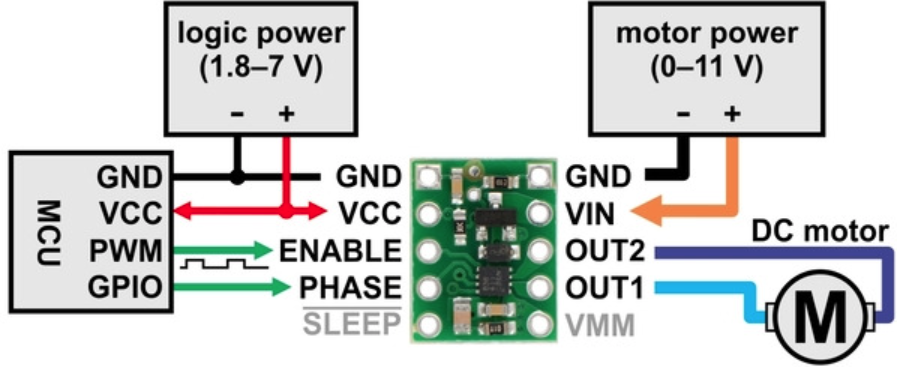
\includegraphics[width=0.6\linewidth]{drv8838.png}
    \caption{Conexionado de la placa de control DRV8838.}
    \label{drv8838}
\end{figure}

Como se observa la placa \gls{DRV8838} tiene múltiples pines. De estos podemos identificar dos grupos: los que aparecen a la izquierda, que llamaremos pines de entrada, y los de la derecha, que denominaremos pines de salida. El \gls{MCU} se conecta a los pines de entrada y, a través de estos, controlará el funcionamiento de la placa. En cambio, en los pines de salida se conecta el motor y transmiten la potencia necesaria.

Dentro de cada uno de estos grupos se encuentran pines destinados a la comunicación entre componentes, y otros que se utilizan para alimentar tanto la lógica de la placa \gls{DRV8838} como al motor. Estos últimos son \textit{GND}, \textit{VCC} y \textit{VIN}. Los pines de control de entrada son \textit{ENABLE}, \textit{PHASE} y \textit{SLEEP}, aunque en este ejemplo se utilizarán solo los dos primeros para simplificar la explicación. De todas formas, en la Tabla \ref{funciones_pin_drv8838} se puede consultar la función de cada pin y si la señal correspondiente es analógica o digital. Por último, \textit{OUT1}, \textit{OUT2} y \textit{VMM} son los pines de salida hacia el motor, y son los que finalmente transmiten la tensión y potencia necesarias para lograr el comportamiento deseado del motor.

\begin{table}[H]
\centering
\begin{tabular}{lllll}
\cline{1-3}
\multicolumn{1}{|l|}{PHASE}  & \multicolumn{1}{l|}{dirección de rotación} & \multicolumn{1}{l|}{digital}   &  &  \\ \cline{1-3}
\multicolumn{1}{|l|}{ENABLE} & \multicolumn{1}{l|}{velocidad de rotación} & \multicolumn{1}{l|}{analógico} &  &  \\ \cline{1-3}
\multicolumn{1}{|l|}{SLEEP}  & \multicolumn{1}{l|}{liberar fuerza}        & \multicolumn{1}{l|}{digital}   &  &  \\ \cline{1-3}
                             &                                            &                                &  & 
\end{tabular}
\caption{Funciones de cada pin del módulo DRV8838}
\label{funciones_pin_drv8838}
\end{table}

\gls{MCU} se conecta a los pines de \textit{ENABLE}, \textit{PHASE} y \textit{SLEEP} el software deberá gestionarlos. Pero, como se mencionó, para acotar el ejemplo se restringieron los requerimientos y para cumplirlos solo necesitaremos trabajar con los pines \textit{ENABLE} y \textit{PHASE}. Tendremos entonces dos cables conectados desde el \gls{microcontrolador} a la placa \gls{DRV8838}, uno que se dirige a \textit{ENABLE} y otro a \textit{PHASE}. En el pseudocódigo \ref{listing1} se encuentran las líneas necesarias para poder configurar el motor para luego poder utilizarlo en el resto del sistema. En estas se establece que el pin número siete del \gls{MCU} está conectado al pin \textit{PHASE} y que el nueve a \textit{ENABLE}. Y a su vez se inicializa el pin dentro del software como pin de salida (\textit{OUTPUT}). Esto es necesario para que otras funciones que se llamen en el futuro se comporten como esperamos.

\begin{lstlisting}[caption=Configuración inicial del control del motor DC.,label={listing1}]
# Notar que los numeros asignados a los pines son arbitrarios dentro del conjunto de pines disponibles en nuestro Arduino.

# Constantes globales
DIR_pin = 7
VEL_pin = 9

def setup()
     .
     .
     .
  pinMode(DIR_pin, OUTPUT)
  pinMode(VEL_pin, OUTPUT)
     .
     .
     .
\end{lstlisting}


Una vez configurados los pines podemos hacer uso de las funciones \verb|pinMode|,\\ \verb|digitalWrite| y \verb|analogWrite| provistas por el entorno de desarrollo de Arduino. Sus nombres son bastantes descriptivos de su comportamiento, \verb|pinMode| configura el modo de operación de un PIN en particular, puede ser \verb|OUTPUT| o \verb|INPUT| (entrada o salida). Y tanto \verb|digitalWrite| como \verb|analogWrite|, configuran en un PIN el valor especificado. \verb|digitalWrite| admite dos valores definidos por el entorno \verb|HIGH| y \verb|DOWN|. Por lo tanto, si se quiere establecer la máxima velocidad de giro en el motor se haría algo como en el Código \ref{codigoMax}. Y en caso de querer detenerlo usamos \verb|analogWrite| de la forma que se muestra en el Código \ref{codigoDet}.

\begin{lstlisting}[caption=Establecer 
máxima velocidad giro en sentido horario.,label={codigoMax}]
digitalWrite(DIR_pin, HIGH)
analogWrite(VEL_pin, 255) # Maximo valor aceptado, PWM siempre encendido
\end{lstlisting}

\begin{lstlisting}[caption=Detener giro del motor DC., label={codigoDet}]
analogWrite(VEL_pin, 0)
\end{lstlisting}

No es necesario entender por completo qué hace cada llamada, pero sí es importante comprender que ejecutar los Códigos \ref{codigoMax} y \ref{codigoDet} es fundamental para controlar el motor. Es decir, cualquier cliente del motor en el sistema debe saber que, para hacer que el motor gire a la máxima velocidad, es necesario ejecutar las dos líneas mostradas en el Código \ref{codigoMax} sobre los pines correspondientes al motor. Por ejemplo, si se desea realizar una acción con el motor en función del valor de alguna variable del sistema (\verb|valor|), \textbf{tradicionalmente} se implementa algo similar al código mostrado en el Código \ref{listingMotor}. En el cual si se cumple la condición de que \verb|valor| es mayor a 100 se ordenará al motor que avance a máxima velocidad, en caso contrario se indicará velocidad nula.

\begin{lstlisting}[caption=Ejemplo uso del motor DC.,label={listingMotor}]
def controlar_motor()

	if (valor > 100)
    	digitalWrite(DIR_pin, HIGH)
	    analogWrite(VEL_pin, 255)
	else
	    analogWrite(VEL_pin, 0)

\end{lstlisting}

¿Qué problemas tiene esta estrategia de cara al cambio?
\begin{itemize}
	\item Consideremos un caso en el que un segundo motor es agregado. Este es controlado por otra placa \gls{DRV8838} que también se conecta con dos pines al \gls{MCU}. Para poder utilizarlo en el código debemos definir al, al igual que con el primer motor, los dos pines que utilizará, supongamos en este caso \verb|DIR_pin2| y \verb|VEL_pin2|. Si queremos modificar la función \verb|controlar_motor| para incluir a este nuevo motor podríamos hacer algo como en el Código \ref{motor2}.
	
\begin{lstlisting}[caption=Extención de la función controlar\_motor para controlar dos motores.,label={motor2}]
def controlar_motor(motor)

	if (valor > 100)
		if (motor = IDMotor1)
    		digitalWrite(DIR_pin, HIGH)
	    	analogWrite(VEL_pin, 255)
	    else if (motor = IDMotor2)
	    	digitalWrite(DIR_pin2, HIGH)
	    	analogWrite(VEL_pin2, 255)
	    	.
	    	.
	    	.
	else
		if (motor = IDMotor1)
	    	analogWrite(VEL_pin, 0)
	    else if (motor = IDMotor2)
	    	analogWrite(VEL_pin2, 0)
	    	.
	    	.
	    	.

\end{lstlisting}
	
La modificación consiste en verificar qué motor es el que se quiere manipular y basándose en eso enviar la señal a través de los pines correspondientes. Pero, ¿qué pasaría si se quiere añadir un tercer motor? Deberíamos agregar aún más sentencias \verb|if else|, extendiendo aún más el código. ¿Y si debemos realizar operaciones diferentes según cada motor? Por ejemplo, en el caso de que \verb|valor| sea mayor a 100 con el motor 1 se debe establecer velocidad máxima pero con el motor 2 nula. El cambio en el código es pequeño (ver Código \ref{motor2mod}), solo cambia un valor en la línea 9. Pero introduce complejidad en la lectura y comprensión facilitando la introducción de errores en futuras modificaciones. Es insostenible en el tiempo este enfoque de diseño.

\begin{lstlisting}[caption=Modificación de la función controlar\_motor para cambiar su comportamiento al utilizar el motor 2.,label={motor2mod}]
def controlar_motor(motor)

	if (valor > 100)
		if (motor = IDMotor1)
    		digitalWrite(DIR_pin, HIGH)
	    	analogWrite(VEL_pin, 255)
		else if (motor = IDMotor2)
	    	digitalWrite(DIR_pin2, HIGH)
	    	analogWrite(VEL_pin2, 0)
	    	.
	    	.
	    	.
	else
		if (motor = IDMotor1)
	    	analogWrite(VEL_pin, 0)
		else if (motor = IDMotor2)
	    	analogWrite(VEL_pin2, 0)
	    	.
	    	.
	    	.

\end{lstlisting}
	\item Imagine el caso en el que por cierto motivo se debe invertir el sentido de giro del motor, de manera que lo que era ir giro horario ahora es antihorario. Para llevar a cabo el cambio, debemos modificar \textbf{todas} las llamadas a \verb|digitalWrite(DIR_pin, HIGH)|, tanto en el código que de la función \verb|controlar_motor| como en el resto del sistema, cambiando \verb|HIGH| por \verb|DOWN| y viceversa. Por ejemplo, en el Código \ref{motor2mod} debemos modificar las líneas 5 y 8. Es fácil cometer un error y dejar al sistema en un estado inconsistente. Ni hablar en el caso que se planteó en el punto anterior, puede ser necesario discriminar entre motores. La precaución a la hora de modificar debe ser mayor aún y a su vez la probabilidad de introducir errores aumenta.
   
    \item Por cierto motivo se descompuso la placa controladora del motor 1, y no se consigue un reemplazo idéntico, sino que se adquiere una nueva placa de otra marca, por ejemplo, una \textit{Pololu Simple Motor Controller G2}. En este caso, esta placa no utiliza la misma interfaz de control que el \gls{DVR8838}, sino para controlarla se accede a ella mediante comunicación serial (utiliza un solo pin específico). Incluso utilizando las herramientas provistas por el entorno de \gls{arduino}, el nuevo código de configuración (ver Código \ref{listingDistinto}) y uso (ver Códigos \ref{maxSerial} y \ref{detSerial}) difiere significativamente del anterior (Codigo \ref{listing1} para configuración y Codigos \ref{codigoMax} y \ref{codigoDet} para uso).
\begin{lstlisting}[caption=Configuración de la placa de control del motor DC utiliza comunicación serie., label={listingDistinto}]
def set_up() 
    .
    .
    .
    Serial.begin(9000)
    .
    .
    .

    \end{lstlisting}
\begin{lstlisting}[caption=Establecer máxima velocidad giro horario para el caso de comunicación en serie., label={maxSerial}]
Serial.write(0xAA)
Serial.write(0x0C)
Serial.write(0x85)
Serial.write(0x7F)
\end{lstlisting}
\begin{lstlisting}[caption=Establecer detención para el caso de comunicación en serie., label={detSerial}]
Serial.write(0xAA)
Serial.write(0x0C)
Serial.write(0xE0)
\end{lstlisting}
Por lo tanto, debemos modificar todos los usos de la antigua implementación por la nueva, lo cual además requerir un esfuerzo considerable, da pie a errores y obliga a reverificar código que ya se sabía que funcionaba correctamente. Se debe modificar las líneas 5, 6 y 15 de la función \verb|controlar_motor| de la manera mostrada en el Código \ref{motor1serial}.

\begin{lstlisting}[caption=Modificación de la función controlar\_motor para utilizar placa de control serial para controlar el motor 1.,label={motor1serial}]
def controlar_motor(motor)

	if (valor > 100)
		if (motor = IDMotor1)
    		Serial.write(0xAA)
				Serial.write(0x0C)
				Serial.write(0x85)
				Serial.write(0x7F)
		else if (motor = IDMotor2)
				digitalWrite(DIR_pin2, HIGH)
	    	analogWrite(VEL_pin2, 0)
	    	.
	    	.
	    	.
	else
		if (motor = IDMotor1)
	    	Serial.write(0xAA)
				Serial.write(0x0C)
				Serial.write(0xE0)
		else if (motor = IDMotor2)
	    	analogWrite(VEL_pin2, 0)
	    	.
	    	.
	    	.

\end{lstlisting}

Pero… ¿Y si en el futuro se consigue la placa \gls{DRV8838}? Muchas veces se suele añadir una bandera que indique el tipo de hardware. En este caso, se podría definir una constante, por ejemplo, \verb|TIPO_MOTOR1|, que identifique el tipo de placa controladora. Al incorporar esta bandera en nuestra función \verb|controlar_motor|, se obtiene el Código \ref{motorBandera}.

\begin{lstlisting}[caption=Modificación de la función controlar\_motor para utilizar bandera indicadora de tipo de placa controladora.,label={motorBandera}]
def controlar_motor(motor)

	if (valor > 100)
		if (motor = IDMotor1)
			if (TIPO_MOTOR1 = DVR8838):
			    digitalWrite(DIR_pin, HIGH)
	    		analogWrite(VEL_pin, 255)
			else if (TIPO_MOTOR1 = Pololu):
    			Serial.write(0xAA)
					Serial.write(0x0C)
					Serial.write(0x85)
					Serial.write(0x7F)
		else if (motor = IDMotor2)
	    	digitalWrite(DIR_pin2, HIGH)
	    	analogWrite(VEL_pin2, 0)
	    	.
	    	.
	    	.
	else
		if (motor = IDMotor1)
			if (TIPO_MOTOR1 = DVR8838):
				analogWrite(VEL_pin1, 255)
			else if (TIPO_MOTOR1 = Pololu):
	    	Serial.write(0xAA)
				Serial.write(0x0C)
				Serial.write(0xE0)
	    else if (motor = IDMotor2)
	    	analogWrite(VEL_pin2, 0)
	    	.
	    	.
	    	.

\end{lstlisting}

Esto no es una buena solución, ya que lo único que logra es generar más dificultad a la hora de introducir un nuevo cambio. Ahora, si se debe cambiar la lógica de la función, debemos tener en cuenta más líneas a modificar. Introduciendo así más posibilidades de cometer errores.

    \item Claramente, el código obtenido es poco claro; es decir, no resulta fácil comprender de qué se trata una determinada porción de código con solo leerla. Basta con intentar entender la función del Código \ref{motorBandera} para comprobarlo. A su vez, el código resulta difícil de modificar, ya que requiere un esfuerzo adicional de comprensión antes de poder aplicar cualquier cambio. En el ejemplo, la lógica principal de la función es sencilla, solo una sentencia condicional, pero en general las funciones suelen ser más complejas e incluyen múltiples sentencias, estructuras anidadas y bucles.


\end{itemize}

En el libro, la solución de este problema es nombrada como un patrón de diseño, el patrón \textit{``Hardware Proxy''}. Pero desde el punto de vista de la IS, no es un patrón de diseño, sino uno de los principios fundamentales de la  IS, que es el \gls{dboi}.

\declareCMod{MotorDC}

Estos inconvenientes son derivados de que el \textit{hardware} comprende un ítem de cambio frecuente; por lo que si seguimos la metodología de Parnas (ver Sección \ref{metoParnas}), se debe aislar ese posible cambio en un módulo. En el ejemplo que se está trabajado, se debe crear un módulo que encapsula el hardware en cuestión, el motor \gls{DC}. Este módulo oculta cómo debe ser usado el hardware y provee una interfaz lo suficientemente insensible a la implementación. Es decir, al momento de confeccionar la interfaz del módulo se debe pensar en lo que el motor siempre va a hacer independientemente de los posibles cambios que sufra el hardware subyacente. Para esto, se debe elegir la cantidad de mínima de métodos del modo más abstracto posible, sin agregar métodos que puedan ser reemplazados utilizando otros que ya fueron definidos \cite{Parnas02, parnas1977abstract}.
Un motor \gls{DC} siempre recibirá órdenes para definir su sentido y velocidad de rotación. La Figura \ref{interfazMotor} presenta la interfaz del módulo \MotorDC que encapsula el hardware relacionado con el motor.

\begin{figure}[H]
\caption{Interfaz MotorDC}
\label{interfazMotor}
\begin{center}
\scalebox{.90}{
\begin{tikzpicture}\sf
\umlclass[x=-3]{MotorDC}
{
MotorDC(i: Pin, i: Pin)
}
{
    
    setDir(i: Dir) \\ 
    setVel(i: Vel) \\
}
\end{tikzpicture}
}
\end{center}
\end{figure}

Si se cuenta con dos o más motores del mismo tipo, se crearán dos a más instancias del módulo. Para esto el constructor recibirá como parámetros los pines de control, el método de \verb|setDir| toma el valor de dirección a establecer y el input de \verb|setVel| el valor de velocidad deseado. En el Código \ref{constructorMotor} se puede ver un ejemplo de una posible implementación de esta interfaz utilizando el controlador \gls{DVR8838}.

\begin{lstlisting}[caption=Posible implementación de la interfaz del módulo MotorDC.,label={constructorMotor}]
def MotorDC(dir_pin, vel_pin);
    pinMode(this.dir_pin, OUTPUT)
    pinMode(this.vel_pin, OUTPUT)


def setDir(dir) 
    if (dir == HORARIO)
        digitalWrite(dir_pin, HIGH)
    else
        digitalWrite(dir_pin, DOWN)
        

def setVel(vel)
    analogWrite(vel_pin, vel)

\end{lstlisting}

En el código \ref{ejeploUsoMotor} se evidencian las primeras ventajas, el uso del motor en el código es mucho más claro en comparación al diseño tradicional, donde teníamos que escribir las líneas de los Códigos \ref{listing1} y \ref{codigoMax} para lograr lo mismo.

\begin{lstlisting}[caption=Ejemplo de uso de la interfaz del módulo MotorDC, label={ejeploUsoMotor}]
motor = MotorDC(1, 2)

motor.setDir(Dir.HORARIO)
motor.setVel(255)
\end{lstlisting}

Además, si se debe invertir el sentido de giro como en el ejemplo propuesto al comienzo de la sección, es tan fácil como cambiar la implementación del método \verb|setDir|, los clientes no notarán el cambio. A su vez, si se quiere controlar otro motor es posible hacerlo fácilmente como en el Código \ref{ejemploOtroMotor}. 

\begin{lstlisting}[caption=Ejemplo control nuevo motor DC.,label={ejemploOtroMotor}]
motor_delantero = MotorDC(18, 19)

motor_delantero.setDir(ANTIHORARIO)
motor_delantero.setVel(10)
\end{lstlisting}


En caso de un cambio de componente de hardware, como el explicado anteriormente, los clientes del módulo no lo notarán, dado que la interfaz se mantendrá intacta. Por ejemplo, para el motor que utiliza comunicación serie, \verb|setDir| será redefinida como en el código \ref{nuevaSetDir} teniendo que solo volver a verificar el módulo \MotorDC.

\begin{lstlisting}[caption=Implementación método setVel para el motor que utiliza comunicación serie.,label={nuevaSetDir}]
def setVel(vel)
        serial.write(0xAA;
        serial.write(0x0C)
        hex_vel = int_to_hex(vel)
        serial.write(hex_vel)
\end{lstlisting}

Sin embargo, haciendo uso del concepto de herencia de interfaz y la noción de abierto-cerrado (explicados en la sección \ref{ingso}). Esto permite reutilizar módulos ya implementados y abstraer aún más la implementación. Para hacerlo se define un módulo abstraco \textit{\MotorDC} del cual hereda la interfaz cada modelo o combinación de motor y placa controladora. La Figura \ref{estructuraHerencia} presenta la estructura de interfaces de esta solución.

\begin{figure}[H]
\caption{Módulo MotorDC abstracto y estructura de herencia.}
\label{estructuraHerencia}
\begin{center}
\scalebox{.90}{
\begin{tikzpicture}\sf
\umlclass[x=0,type=abstract]{MotorDC}
{}
{
    \umlvirt{setDir(i: Dir)} \\ 
    \umlvirt{setVel(i: Vel)} \\
}

\umlclass[x=-3, y=-4]{MotorDCDVR8838}
{
	MotorDC(i: Pin, i: Pin)
}
{
    setDir(i: Dir) \\ 
    setVel(i: Vel) \\
}
\umlclass[x=3, y=-4]{MotorDCG2}
{
	MotorDC(i: Serial)
}
{
    setDir(i: Dir) \\ 
    setVel(i: Vel) \\
}
\umlinherit[geometry=|-|]{MotorDCDVR8838}{MotorDC}
\umlinherit[geometry=|-|]{MotorDCG2}{MotorDC}
\end{tikzpicture}
}
\end{center}
\end{figure}

El cliente solo sabe que manipula un elemento \textit{\MotorDC}, no tiene noción con cuál de los dos tipos de placa controladora está tratando. También es posible agregar más herederos, uno por cada modelo de placa controladora/motor, y reutilizar los módulos implementados en caso de utilizar hardware idéntico.

Siguiendo con el ejemplo de la función \verb|controlar_motor| veamos en la Figura \ref{motorEncapsulado} cómo es una posible implementación de esta misma utilizando la encapsulación del hardware propuesta. Con esta solución el código de la función no deberá ser modificado por más que cambien las marcas/tipos de placas controladoras.

\begin{lstlisting}[caption=Implementación de la función controlar\_motor utilizando encapsulación del hardware.,label={motorEncapsulado}]
def controlar_motor(motor: MotorDC)
	if (valor > 100)
		motor.setDir(HORARIO)
		motor.setDir(VelMaxima)
	else
		motor.setDir(VelNula)
\end{lstlisting}

De esta manera se siguen las prácticas recomendadas en la \gls{IS} \cite{ShawGarlan1996, ghezzi2003, bass2003, DBLP:books/daglib/0030743} y se obtiene un diseño orientado al cambio \cite{Gamma:1995:DPE:186897}.

\section{Interfaces que no se ajustan perfectamente}
Muchas veces el proveedor del hardware incluye con estas librerías para su control, otras veces se consiguen en internet o se extraen de previos proyectos. Esto permite ahorrar tiempo de implementación, pero puede causar algunos inconvenientes si no se tiene en cuenta al cambio.

Tradicionalmente, se toman las librerías necesarias para controlar el hardware y se las utiliza directamente a lo largo del sistema. Lo que provoca que ante un cambio de hardware se debe modificar todos los usos de la librería con el nuevo código. Veamos un ejemplo en donde se evidenciará el inconveniente y cómo podemos anticiparnos al mismo.

Suponga el siguiente ejemplo: en un cierto sistema embebido se utiliza un display de 7 segmentos que forman un 8. Encendiendo o apagando independientemente cada segmento, se pueden mostrar distintos caracteres. Este display es de 4 dígitos y se emplea para mostrar la temperatura de funcionamiento y la posición, en grados, de cierto actuador, como se muestra en la figura \ref{fig:enter-label}.

\begin{figure}[h]
    \centering
    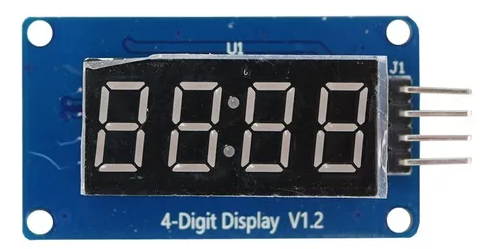
\includegraphics[width=0.4\linewidth]{display.png}
    \caption{Display 7 segmentos 4 digitos}
    \label{fig:enter-label}
\end{figure}

\declareCMod{LibAcme}
\declareCMod{LibEmca}

Este display recibe la información utilizando comunicación en serie, con un protocolo propio del fabricante. Para facilitar su uso, el fabricante brinda una librería llamada \LibAcme que implementa la comunicación y provee funciones simples de usar, tales como \verb|escribir(i: string): bool| y \verb|limpiar()|. La primera intenta escribir la cadena de caracteres indicada, pero solo lo hace si el display no está mostrando nada. En ese caso devuelve \verb|True| indicando que la acción fue completada con éxito. En caso contrario, es decir el display está mostrando texto al momento de llamar el método, retorna \verb|False|. \verb|limpiar()|, siempre limpia el display. Por lo tanto, se implementó el sistema utilizando las funciones provistas. Para comunicarse, múltiples módulos llaman esas funciones de la manera expuesta en el Código \ref{usoLibAcme}.

\begin{lstlisting}[label={usoLibAcme}, caption=Ejemplo de uso de la libreria LibAcme.]
libAcme = LibAcme()

if libAcme.escribir("24")
	print("El display estaba vacio, se pudo escribir el nuevo texto")
else
	print("El display esta ocupado mostrando algo, no se pudo escribir")

\end{lstlisting}

En cierto momento, el módulo display dejó de funcionar y fue reemplazado por otro de un fabricante distinto, el cual utiliza un protocolo de comunicación diferente. Al igual que en el caso anterior, la empresa provee una librería \LibEmca para utilizar el nuevo display. Sin embargo, la interfaz no es la misma que la anterior, e incluso algunos comportamientos también difieren.

Por ejemplo, en la primera librería, el método de escritura devolvía \verb|False| si se intentaba escribir mientras el display ya estaba mostrando información. En cambio, en la nueva implementación, si el display está mostrando algo, el nuevo texto lo sobrescribe de inmediato. No obstante, esta nueva librería proporciona un método adicional \verb|get_current(): string| que permite consultar el contenido que se está mostrando en el momento en que es invocado.

Tradicionalmente, para utilizar el nuevo display, se modifican todas las llamadas a las funciones de la librería anterior en todo el sistema, incorporando la nueva lógica. En nuestro ejemplo, el Código \ref{usoLibAcme} debe ser reemplazado por el Código \ref{usoLibEmca}. Si bien el cambio puede parecer superficial, es importante considerar que con cada modificación será necesario actualizar manualmente y reverificar \textbf{todos} los usos de la librería a lo largo del sistema.
\begin{lstlisting}[label={usoLibEmca}, caption=Ejemplo de modificaciones necesarias para adaptar la nueva librería.]
libEmca = LibEmca()

// Con EMCA

if libEmca.get_current() == ""
	libEmca.imprimir("Hola mundo!")
	print("El display estaba vacio, se pudo escribir el nuevo texto")
else
	print("El display esta ocupado mostrando algo, no se pudo escribir")


\end{lstlisting}

Además, este es un ejemplo simple; en el mundo real, los cambios pueden ser mucho más complejos en su lógica y de distinta naturaleza. Este diseño puede representarse como se muestra en la Figura \ref{configOri}: un módulo que constituye la librería del fabricante y otro que actúa como cliente de esta, es decir, el resto del sistema.


\begin{figure}[H]
\caption{Diseño tradicional del uso de la librería del fabricante.}
\label{configOri}
\begin{center}
\scalebox{.90}{
\begin{tikzpicture}\sf
\umlsimpleclass[]{Cliente}

\umlclass[right=1.5cm of Cliente]{LibAcme}
{}
{
escribir(i: string): bool  \\
limpiar()
}

\umluniassoc[]{Cliente}{LibAcme}


\umlnote[below left=0.5cm and 0.5cm of LibAcme, width=3cm]{LibAcme}{
Librería externa.
}


\end{tikzpicture}
}
\end{center}
\end{figure}

Este diseño presenta un fuerte acoplamiento entre el \Cliente y la \LibAcme, por lo que cualquier cambio en el hardware repercutirá en el resto del sistema, trayendo consigo todas las desventajas mencionadas tanto en este capítulo como en el anterior. Se podría decir que el principal problema radica en que no se siguió la metodología de diseño propuesta por Parnas \cite{Parnas1972}. El hardware representa un ítem con alta probabilidad de cambio, por lo tanto, debe ser encapsulado.

En el libro de Douglass \cite{douglass} se observa que, en la práctica, este tipo de escenarios son comunes: ya se tiene un sistema funcionando y se produce un cambio de hardware. Por ello, se intentará proponer una posible solución desde el punto de vista de la \gls{IS}. En lugar de reescribir todo el sistema, veremos cómo, aplicando un patrón de diseño de Gamma \cite{Gamma:1995:DPE:186897}, es posible adaptar el sistema y preparar el diseño del mismo para futuros cambios de índole similar.
\declareAMod{Display}
Para encapsular el hardware sin modificar todo el sistema se creará un módulo abstracto llamado \Display. En su interfaz proveerá los mismos métodos que \LibAcme de esta manera evitaremos cambiar la implementación del resto del sistema. Al compartir interfaz podemos decir que \LibAcme hereda la interfaz de \Display, esto lo podemos ver en la Figura {configUsando}.

\begin{figure}[H]
\caption{Introducción del nuevo módulo abstracto\Display.}
\label{configUsando}
\begin{center}
\scalebox{.90}{
\begin{tikzpicture}\sf
\umlsimpleclass[]{Cliente}

\umlclass[right=1.5cm of Cliente,type=abstract]{Display}
{}
{
\umlvirt{escribir(i: string): bool}  \\
\umlvirt{limpiar()}
}

\umlclass[right=0.5cm of Cliente,below=2cm of Cliente]{LibAcme}
{}
{
escribir(i: string): bool  \\
limpiar()
}

\umluniassoc[]{Cliente}{Display}
\umlinherit[geometry=|-|]{LibAcme}{Display}


\end{tikzpicture}
}
\end{center}
\end{figure}
\declareCMod{DisplayEmca}
Como mencionamos, \LibEmca se utiliza para controlar el nuevo display, pero su interfaz y funcionalidad no son las mismas que las de \LibAcme. Por lo tanto, aplicaremos el patrón \textit{Adapter} (Adaptador) propuesto por Gamma \cite{Gamma:1995:DPE:186897}. Este patrón consiste, en este caso, en crear un módulo \DisplayEmca, que se encarga de adaptar la interfaz de \LibEmca a la de \Display. Es decir, utilizará los métodos de \LibEmca para implementar la funcionalidad esperada por los métodos de \Display. De esta manera, se obtiene la estructura de módulos mostrada en la Figura \ref{configNueva}.

\begin{figure}[H]
\caption{Diseño aplicando el patrón \textit{Adapter}.}
\label{configNueva}
\begin{center}
\scalebox{.90}{
\begin{tikzpicture}\sf
\umlsimpleclass[x=-4.5,y=1]{Cliente}

\umlclass[x=0,y=1,type=abstract]{Display}
{}
{
\umlvirt{escribir(i: str): bool}  \\
\umlvirt{limpiar()}
}
\umlclass[x=-2.5,y=-3]{LibAcme}
{}
{
escribir(i: str): bool  \\
limpiar()
}
\umlclass[x=2.5,y=-3]{DisplayEmca}
{}
{
escribir(i: str): bool  \\
limpiar()
}
\umlclass[x=8,y=0.5]{LibEmca}
{}
{
imprimir(i: str)  \\
get\_current(): str
}
umluniassoc
\umlinherit[geometry=|-|]{LibAcme}{Display}
\umlinherit[geometry=|-|]{DisplayEmca}{Display}
\umluniassoc[]{Cliente}{Display}
\umluniassoc[geometry=-|-]{DisplayEmca}{LibEmca}

\umlnote[below=0.5cm of LibEmca, width=3cm]{LibEmca}{
Librería externa.
}
\end{tikzpicture}
}
\end{center}
\end{figure}

No olvidar que cada aplicación de un patrón de diseño debe ser seguida por su correspondiente documentación \textbf{2MIL}. En este caso se la presenta en la Figura \ref{docAdapter}.

\begin{figure}[H]
\caption{Documentación de la aplicación del patrón Adapter al ejemplo del display.}
\label{docAdapter}
\scalebox{.90}{
\begin{pattern}[]{Adaptar nuevo controlador de display}{Algorithm}{idFigAlg}
\based{Adaptador (Adapter)}
\why{\textbf{Cambios previstos}: Se pueden agregar diferentes displays pero manteniendo una interfaz común.

\textbf{Funcionalidad}: En caso de agregar un nuevo display que provee una interfaz diferente a la utilizada en el sistema, se crea un módulo que la adapta para que corresponda a la usada.
}
\assigns
\is{Display}{Target}
\is{LibEmca}{Adaptee}
\is{DisplayEmca}{Adapter}
\end{pattern}
}
\end{figure}


En el Código \ref{codigoAdapter} se presenta un ejemplo de implementación del módulo \DisplayEmca. En este se utilizan los métodos provistos por la librería del fabricante, y se emula la interfaz de \Display. De este modo, se permite reemplazar el hardware sin necesidad de modificar ni reverificar ninguna otra parte del sistema.

\begin{lstlisting}[label={codigoAdapter}, caption=Ejemplo de implementación del módulo \ControlEmca]
escribir(string palabra)
    if (libEmca.get_current() != "")
        return false
	else
    	libEmca.imprimir(cadena)
    	return true

limpiar()
    libEmca.imprimir("")
\end{lstlisting}

Las ventajas de aplicar este patrón en esta situación particular en la cual se parte de un diseño \textbf{no} orientado al cambio son:

\begin{itemize}

\item Facilitar la sustitución de hardware: permite cambiar el display sin necesidad de modificar el código del cliente, reduciendo el impacto del cambio de hardware en el sistema.

\item Mantener la coherencia en la interfaz: el cliente sigue interactuando con la misma interfaz abstracta (\Display), evitando la necesidad de modificar múltiples módulos en el sistema.

\item Minimizar el riesgo de errores: al encapsular las diferencias de implementación en el adaptador (\DisplayEmca), se reduce la posibilidad de introducir errores al modificar manualmente todas las llamadas en el código.

\item Mejorar la mantenibilidad: cualquier nuevo display con una librería de control solo requiere la creación de un nuevo adaptador.

\item Se promueve la reutilización de código: la abstracción permite reutilizar la lógica del cliente sin importar qué display se use, evitando la duplicación de código y mejorando la modularidad.
\end{itemize}


\section{Obtención de información}
\label{obtInfo}

Generalmente, una tarea importante que tienen los sistemas embebidos es recavar información proveniente de sensores. Existen diferentes formas en las que los sensores transmiten información al sistema. Algunos, por ejemplo un sensor de temperatura, establece en el pin en el que está conectado un valor de tensión, por lo que el sistema solo debe consultar el valor del pin. Otros, en cambio, se comunican mediante interrupciones; por ejemplo un sensor de efecto \gls{hall} genera una interrupción por cada detección de campo magnético. Por lo tanto, si lo estamos usando para calcular las \gls{RPM} de un componente giratorio, debemos llevar una cuenta de las interrupciones que generó en cierto periodo de tiempo y realizar una operación matemática. Evidentemente, es necesario que alguna porción de nuestro sistema se encargue de hacerlo y maneje las interrupciones generadas por el sensor. Algo similar pasa con otros tipos de dispositivos como joysticks, botones, etc.

Tradicionalmente, esta tarea se centraliza en un único módulo que provee dos métodos: uno encargado de manejar la interrupción, procesar y almacenar la información, y otro que se utiliza para acceder a ella. Al aplicar esta solución, se obtiene una estructura poco resiliente al cambio. Por ejemplo, si se modifican los cálculos para obtener el resultado deseado, es necesario modificar también la implementación del módulo, lo que da lugar a la posible introducción de errores. Asimismo, la manera de transmitir la información relacionada con la interrupción puede variar debido a modificaciones en el hardware (tipo o modelo del sensor, componentes mecánicos, etc.). En \gls{IS}, decimos que el módulo oculta más de un ítem de cambio y, como vimos previamente, esto no se ajusta a las prácticas recomendadas.

Además, en muchos casos ni siquiera se construye este módulo, sino que cada cliente del dispositivo se encarga de capturar y procesar los datos provenientes, lo que provoca que, ante cualquier cambio, deba modificarse el código en diferentes módulos a lo largo del sistema.

Es debido a las problemáticas mencionadas que resulta útil contar con una forma general de abordar este problema desde el punto de vista del diseño orientado al cambio. Para ello, tomaremos como referencia el trabajo realizado sobre el robot desmalezador en \cite{paperPomponio}, en el cual se empleó la estructura modular presentada en la Figura \ref{activo}, destinada a llevar a cabo las actividades necesarias para el uso de sensores que generan interrupciones en el sistema. Replicaremos esta estructura, siguiéndola casi como si fuera un patrón de diseño.

\begin{figure}[H]
\caption{Estructura componentes para la lectura de un sensor activo.}
\label{activo}
\centering
\scalebox{.90}{
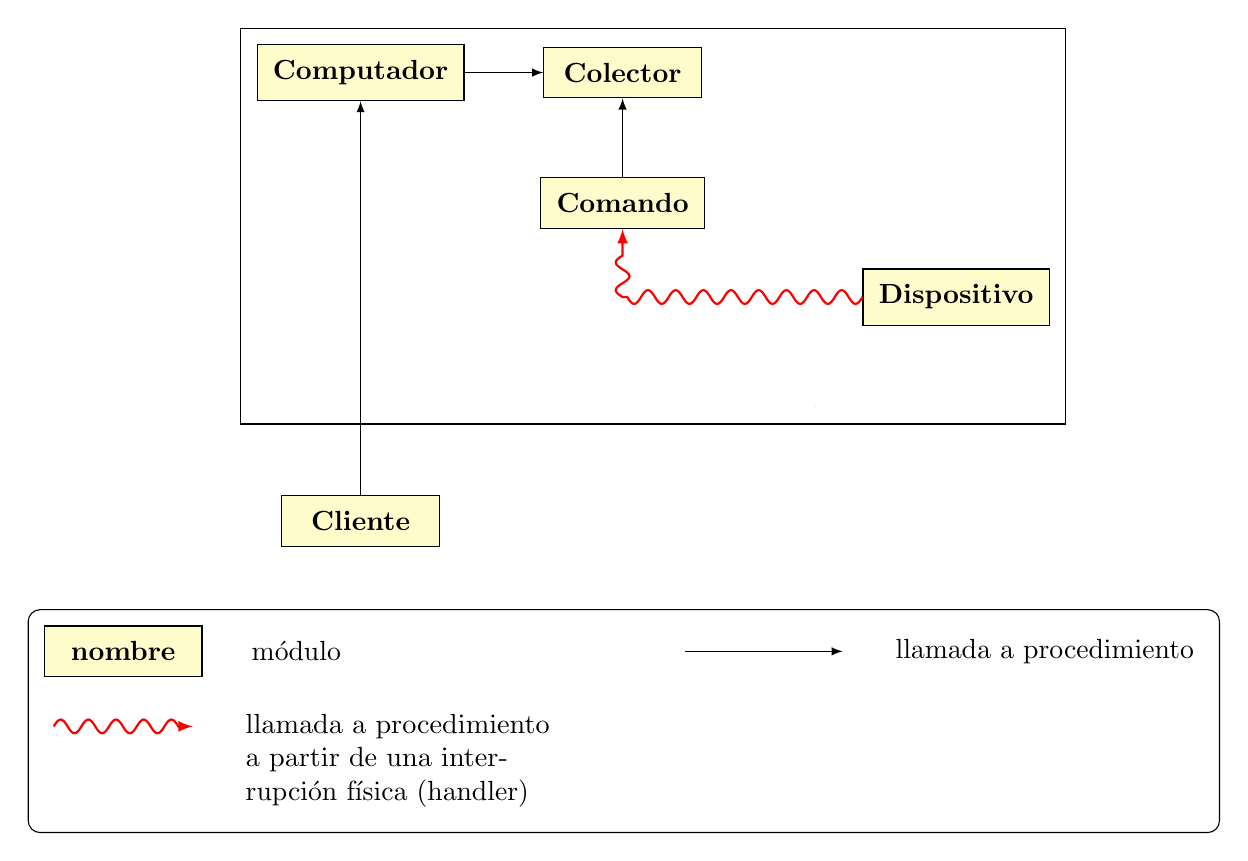
\begin{tikzpicture}\hypertarget{fig:ConnectBufferToMCU}{}
%-------------Estilos para dibujar-----
\tikzstyle{módulo}=[minimum width=1cm,inner sep=2mm,above right,draw,align=center,minimum width=2cm, font=\bfseries]

\tikzstyle{supest}=[rounded corners=1.5mm, minimum width=2cm,inner sep=2mm,draw,text width=2cm]

\tikzstyle{componente}=[minimum width=2cm,inner sep=2mm,draw,text width=2cm]

\tikzstyle{nombre}=[inner sep=0mm, font=\bfseries]

\tikzstyle{pipe}=[-latex,thick,line width=4pt]

\tikzstyle{modExt}=[minimum width=1cm,inner sep=2mm,above right,draw, dotted,line width=2pt,align=center,minimum width=2cm,color=gray, font=\bfseries]

\tikzstyle{flechaFisica}=[-latex,snake=coil,segment aspect=0, red, thick];
%--------------------------

\node[módulo,fill=yellow!20](Pin){Dispositivo};

\node[módulo, above left=0.5cm and 2cm of Pin, fill=yellow!20](CountTime){Comando};

\draw[flechaFisica](Pin) -| (CountTime);

\node[módulo, above=1cm of CountTime, fill=yellow!20](CRpinCollector){Colector};

\draw[-latex](CountTime) edge (CRpinCollector);

\node[módulo, left=1cm of CRpinCollector, fill=yellow!20](CRBuffer){Computador};

\draw[-latex](CRBuffer) edge (CRpinCollector);

\node[módulo, below=5cm of CRBuffer, fill=yellow!20](BufferReader){Cliente};

\draw[-latex](BufferReader) edge (CRBuffer);

\node[nombre, below right = 1cm and -3cm of Pin, fill=yellow!20](ConnectBufferToMCU){};

\node[componente, fit=(Pin)(CountTime)(CRBuffer)(ConnectBufferToMCU)]{};

%%------------------------------Referencias------------

\node[módulo, below left=1cm and 1cm of BufferReader, fill=yellow!20](mod){nombre};
\node[right =0.5cm of mod](modDesc){módulo};

\node[right=4cm of modDesc](x1){};
\node[right=2cm of x1](x2){};
\draw[-latex](x1)--(x2);
\node[right=0.3cm of x2](llp){llamada a procedimiento};

\node[below=0.5cm of mod.south west](x1a){};
\node[below=0.5cm of mod.south east](x2a){};
\draw[flechaFisica](x1a)--(x2a);
\node[below right=-0.4cm and 0.3cm of x2a, text width=4cm](hand){llamada a procedimiento a partir de una interrupción física (handler)};

%
\node[supest, fit=(mod)(hand)(llp)]{};

\end{tikzpicture}
}
\label{fig:ConnectBufferToMCU}
\end{figure}

\declareCMod{Dispositivo}
\declareCMod{Colector}
\declareCMod{Computador}
\declareCMod{Comando}

En esta estructura se distinguen cuatro módulos principales: \Dispositivo, que encapsula el hardware asociado al dispositivo encargado de generar e introducir la interrupción. Este módulo cuenta con un manejador de interrupción configurado para invocar al comando encapsulado en el módulo \Comando cuando la interrupción es lanzada. Este último sigue el patrón de diseño \textit{Command} y ejecuta los métodos del módulo \Colector para registrar la información requerida sobre la interrupción (por ejemplo, el momento exacto en que ocurrió el evento o la cantidad de veces que sucedió). De este modo, podemos deducir que \Colector almacena la información ``cruda'' proveniente de la interrupción o del sensor. Finalmente, se encuentra el módulo \Computador, encargado de procesar la información cuando esta es solicitada. Para ello, lee los valores almacenados en \Colector y aplica cálculos o algoritmos que computan la información final aportada por el dispositivo. Un ejemplo de ello podría ser el cálculo de la velocidad de rotación de una rueda o la obtención de los inputs de un joystick.

A continuación se presenta un ejemplo de aplicación con el objetivo de analizar en mayor profundidad la estructura modular. Se considera un sensor de efecto \gls{hall} montado de manera tal que, al girar una rueda, imanes permanentes pasen cerca de este. De esta forma, el sensor puede utilizarse para medir la velocidad de rotación. En la Figura \ref{hall} se observa la variación de voltaje producida por el paso de los imanes frente al sensor. Cada vez que el dispositivo detecta un campo magnético, emite una interrupción que es gestionada por el módulo \Comando, el cual actúa como un comando y, por lo tanto, conoce qué funciones ejecutar dentro del módulo \Colector.

\begin{figure}[H]
    
    \caption{Ejemplo de la variación de voltaje producida por un sensor de efecto Hall al detectar un cambio del campo magnético. Cada pico de voltaje provoca que el microcontrolador genere una interrupción. Imagen extraída de \cite{disenioViejo2}.}
    \centering
    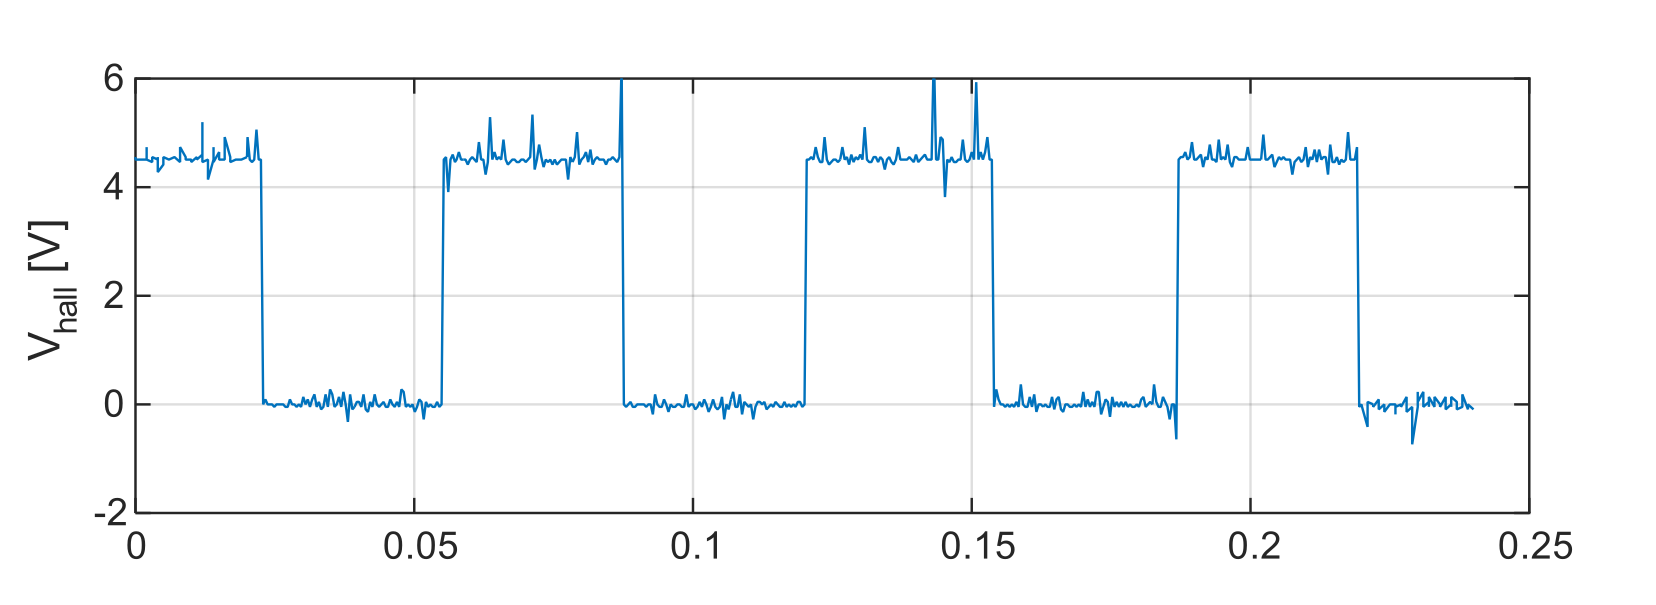
\includegraphics[width=0.8\linewidth]{sensorHall.png}
    \label{hall}
\end{figure}

\declareCMod{SensorVelocidad}

En la Figura \ref{estructuraHall} se presenta la estructura de módulos de esta solución, junto con pseudocódigo que ilustra una posible implementación.

Con los imanes colocados a una distancia conocida, para calcular la velocidad es necesario registrar los dos últimos instantes de tiempo en que fueron detectados. De forma simplificada, la velocidad se obtendrá al dividir la distancia entre los imanes por el tiempo transcurrido entre ambas detecciones. En consecuencia, el módulo \Colector debe proveer un método para almacenar el momento de cada detección. Posteriormente, el módulo \SensorVelocidad, que cumple la función de \Computador, tomará la información almacenada en \Colector y realizará el cálculo matemático para determinar la velocidad de giro de la rueda. Los cálculos, que pueden ser complejos, se ejecutarán únicamente bajo demanda, es decir, cuando el cliente lo requiera. Esto permite optimizar el rendimiento del sistema al disminuir la carga computacional necesaria. Cabe aclarar que este ejemplo está simplificado y omite situaciones que conllevarían una complejidad innecesaria.

\begin{figure}[H]
\caption{Ejemplo módulos para obtener la información referida a la velocidad.}
\label{estructuraHall}
\centering
\begin{center}
\scalebox{.90}{
\begin{tikzpicture}\sf

\umlclass[]{SensorHall}
{}
{
start()\\
stop()\\
signalHandler() \\
setCommand(i: Command)
}

\umlnote[above=1cm of SensorHall,width=3cm]{SensorHall}
{
signalHandler() \{\\
\ \ \ \ cmd.execute() \\
\}
}

\umlclass[above left=1cm and 2cm of SensorHall]{Count}
{}
{
execute() \\
}

\umlnote[below left=2.5cm and -1cm of Count,width=4cm]{Count}
{
Hereda de Command \\
execute() \{ \\
\ \ \ colector.addEvent() \\
\}
}

\umlclass[above=1cm of Count]{Colector}
{}
{
addEventTime() \\
getLastEventTime() \\
getSndLastEventTime() \\
}

\umlclass[left=2cm of Colector]{SensorVelocidad}
{
Buffer(i: Colector)
}
{
getVelocidad()
}

\umlnote[below=1cm of SensorVelocidad,width=7.5cm]{SensorVelocidad}
{
getVelocidad() \{ \\
\ \ \ last = colector.getLastEventTime() \\
\ \ \ second = colector.getSndLastEventTime() \\
\ \ \ return DISTANCIA / (last - second) \\
\}
}

\umlnote[right=1cm of Colector,width=5.5cm]{Colector}
{
addEventTime() \{ \\
\ \ \ secondLast = last \\
\ \ \ last = time.getCurrentTime() \\
\}

}

\umluniaggreg[arg1=colector,pos1=0.5]{SensorVelocidad}{Colector}
\umluniaggreg[geometry=-|]{SensorHall}{Count}

\end{tikzpicture}
}
\end{center}
\end{figure}

Al aplicar esta solución orientada al cambio, preparamos esta sección del sistema para cambios probables, tanto de hardware como de algoritmos. Además, las responsabilidades se separan en módulos independientes, logrando que una modificación en uno de ellos no afecte al resto del sistema. De este modo, si la rueda fuera modificada y cambiara la distancia entre los imanes, bastaría con actualizar la implementación del módulo \SensorVelocidad. A su vez, si el sensor \gls{hall} fuese reemplazado, solo se cambiaría el módulo que lo encapsula, manteniendo intacto el resto de la aplicación.

En esencia, las ventajas obtenidas con este diseño impactan directamente en la sostenibilidad y el ciclo de vida del software. Al lograr este nivel de bajo acoplamiento y alta cohesión, se minimiza el costo y el riesgo asociados al mantenimiento, ya que los cambios quedan confinados y son esperados. Esto no solo previene la propagación de errores, sino que genera que el sistema tenga una alta resiliencia y flexibilidad.


\subsubsection*{Recolectar información de manera periódica.}

Algunos sistemas se encargan de mostrar, almacenar o verificar la información de los sensores a intervalos regulares. En estos casos no resulta crítico perder valores intermedios, es decir, no se requiere una respuesta inmediata. Un ejemplo de ello puede ser una estación meteorológica o un dispositivo médico de monitorización, como un tensiómetro que registra los valores de presión del paciente cada cierto período.

Una implementación intuitiva consiste en escribir un \textit{loop} en el que se verifique la información de los sensores, llamando a métodos que la obtengan directamente del hardware, para luego ejecutar una función \textit{sleep} que bloquea el programa durante un tiempo determinado. Este enfoque presenta varias desventajas: en primer lugar, el tiempo de ejecución de la propia rutina alarga el período; en segundo lugar, si se desean agregar otras funcionalidades durante la espera, es necesario dividir la llamada a \textit{sleep} y recalcular los tiempos de ejecución.

Una solución más adecuada desde el punto de vista del diseño orientado al cambio es la siguiente: se configura un temporizador para que, cada \textit{x} cantidad de tiempo, genere una interrupción. Esta es una funcionalidad provista por muchos entornos de desarrollo para sistemas embebidos, como \gls{arduino}.
Para dicha interrupción, se registrará un manejador que consistirá en un módulo implementado según el patrón de diseño \textit{Command} (ver Sección \ref{patronCommand} para más información sobre este tipo de aplicación del patrón). Este encapsula las funciones que deben ejecutarse para llevar a cabo la funcionalidad deseada como, por ejemplo, solicitar la información a sus respectivos módulos \Computador o a los sensores en sí, para luego registrarla en un cierto módulo que oculte la estructura de datos. De esta forma, se logra liberar al procesador durante los tiempos de espera y desacoplar esta funcionalidad.


\section{Máquinas de estado}\label{cap:state}

Muchos sistemas ajustan su comportamiento durante su ejecución en función de diversas causas, como interacciones con el entorno o requisitos internos. Un ejemplo sencillo es un sistema de control de microondas, que no iniciará el calentamiento si la puerta está abierta. En este caso, la condición de la puerta representa un estado interno que restringe un comportamiento (calentar) mientras permite otro. Del mismo modo, el comportamiento de un motor en un robot está determinado por su estado de dirección, que puede ser ``giro horario'' o ``giro antihorario''. Otro ejemplo es un sistema en el que, al finalizar una operación, se cambia del estado trabajando al estado esperando, lo que también altera el comportamiento del sistema. De manera similar, un sistema de climatización puede estar en estado calentando o enfriando, dependiendo de la configuración del termostato. Por lo tanto, la gestión de estados, sus transiciones y los cambios de comportamiento asociados a estos son aspectos fundamentales en el diseño de sistemas complejos y representan un ítem de cambio bastante probable.

Una solución de implementación tradicional para gestionar estados consiste en almacenarlos en una variable. Posteriormente, se verifica el valor de esta variable para modificar el comportamiento de las funciones, como se ilustra en el código \ref{codigoMicro}.

\begin{lstlisting}[label=codigoMicro,caption={Ejemplo de manejo de estados tradicional, en el caso del microondas.}]
calentar():
    if (estado == PuertaAbierta):
        return
    else if (estado == Preparado):
        magnetron.encender()
    else if (estado == Pausa):
    	magnetron.encender()

\end{lstlisting}

Este enfoque, si bien es directo, presenta varias desventajas al modificar o extender el código. Por ejemplo, al agregar nuevos estados o cambiar el comportamiento del sistema, la gestión se vuelve rápidamente compleja. Esta creciente complejidad es una de las principales desventajas de su implementación. A medida que se añaden más estados, cada método requiere más verificaciones, lo que conduce a una proliferación de estructuras \textit{if-else}. Esto no solo dificulta la lectura del código, sino que también aumenta la probabilidad de introducir errores, ya que cada nuevo estado debe ser cuidadosamente incorporado y verificado en todas las partes relevantes del sistema. Además, este enfoque compromete la sostenibilidad del software. En el Código \ref{nuevoEstado} se muestra cómo se agrega un nuevo estado al método \verb|calentar()|.

\begin{lstlisting}[label=nuevoEstado,caption={Ejemplo de introducción de un nuevo estado a la solución tradicional.}]
calentar():
    if (estado == PuertaAbierta):
        return
    else if (estado == Preparado):
        magnetron.encender()
    else if (estado == Pausa):
    	magnetron.encender()
    else if (estado == Calentando):
    	magnetron.apagar()

\end{lstlisting}

Cuando el comportamiento de un estado debe cambiar, es posible que se necesiten modificaciones en múltiples métodos. Esto puede llevar a la duplicación de código o dificultar la identificación de las partes que requieren cambios, complicando el proceso y aumentando el riesgo de errores. 

Otra desventaja clave es la baja modularidad, ya que el comportamiento asociado a cada estado no está claramente delimitado. Si cada estado requiere comportamientos complejos, el código se vuelve monolítico y difícil de extender sin alterar los métodos existentes. Por ejemplo, al agregar un estado \textit{EnPausa}, sería necesario modificar la lógica de múltiples métodos para verificar este nuevo estado y ajustar el comportamiento de manera apropiada. Todas estas deficiencias dificultan la reutilización del código y hacen que la verificación del correcto funcionamiento del sistema sea cada vez más compleja.

Este tipo de solución es ampliamente utilizado. Un ejemplo relevante se encuentra en el software original del robot desmalezador, como se describe en el informe \cite{informe1}. En particular, se definen diferentes estados de operación del robot y se utiliza una gran estructura de control \textit{switch-case} dentro del bucle principal. Esta estructura decide la acción a ejecutar en función del estado actual, como se detalla en el Código \ref{codigoLoopMain}.

\begin{lstlisting}[caption=Main loop del previo firmware del robot desmalezador \cite{informe1}, label={codigoLoopMain}]
switch (ESTADO) {
	case DUTY_REMOTO:
		duty_remoto();
		break;
	case RPM_REMOTO:
		rpm_remoto();
		break;
	case DUTY_PC:
		duty_pc();
		break;
	case RPM_PC:
		rpm_pc();
		break;	
	case CALIBRACION:
		calibracion();
		break;
	case PERDIDA_SENAL:
		perdida_senal();
		break;
	case EMERGENCIA:
		EMERGENCY();
		break;
	default:
		ESTADO = PERDIDA_SENAL;
		break;
}
\end{lstlisting}

Antes de abordar una perspectiva de diseño para gestionar el cambio, se analizará en detalle el ejemplo presentado en el libro de Douglass \cite{douglass} y la aplicación de una otra solución al manejo de estados.

El ejemplo propuesto consiste en el sistema de control de un microondas. Para representar el comportamiento del mismo, el autor presenta una máquina de estados como la de la Figura \ref{maquinaMicroondas}. Aunque contiene algunas incoherencias y no es del todo exacta, es suficiente para el propósito del ejemplo que se busca exponer.

\begin{figure}[h]
\caption{Máquina de estados extraída del libro \cite{douglass}.}
\label{maquinaMicroondas}
\begin{center}
\scalebox{.90}{
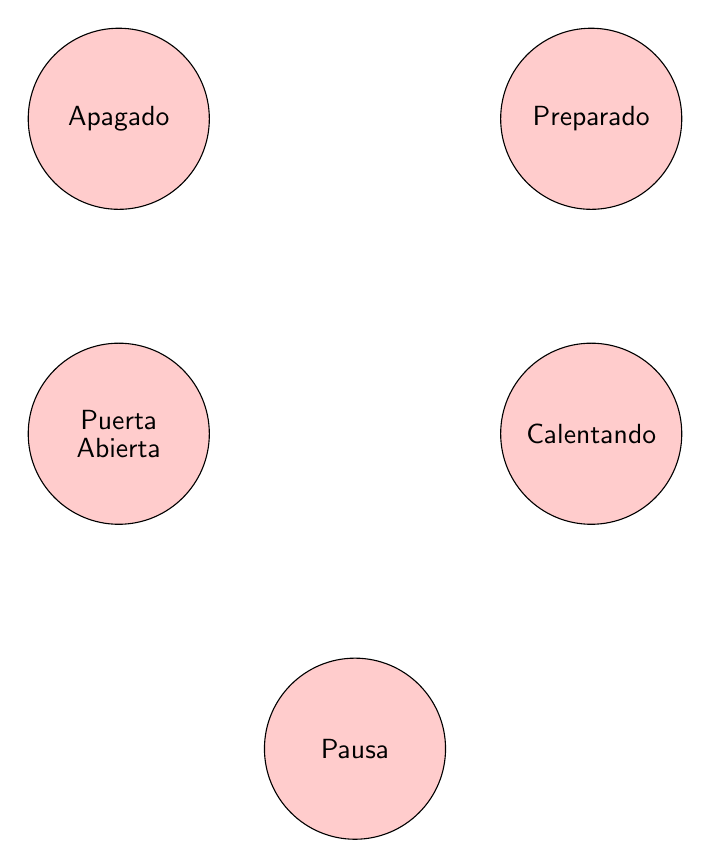
\begin{tikzpicture}[umlstate/.style={
    circle,
    draw,
    minimum size=2.3cm,
    fill=red!20,
    font=\sffamily
}]

\node[umlstate] (Apagado) at (-3,0) {Apagado};
\node[umlstate] (Preparado) at (3,0) {Preparado};
\node[umlstate] (PuertaAbierta) at (-3,-4) {\shortstack{Puerta\\Abierta}};
\node[umlstate] (Calentando) at (3,-4) {Calentando};
\node[umlstate] (Pausa) at (0,-8) {Pausa};

\umltrans[arg=prender, pos=0.5] {Apagado}{Preparado}
\umltrans[arg=cancelar, pos=1.5, geometry=|-|, anchor2=-120] {PuertaAbierta}{Preparado}
\umltrans[arg=calentarTemp, anchor1=-60, anchor2=60, pos=0.3] {Preparado}{Calentando}
\umltrans[arg=tempListo, pos=0.3] {Calentando}{Preparado}
\umltrans[arg=cerrar, pos=0.5,anchor1=10, anchor2=170] {PuertaAbierta}{Calentando}
\umltrans[arg=abrir, pos=0.5,anchor1=-170, anchor2=-10] {Calentando}{PuertaAbierta}
\umltrans[arg=abrir, pos=1.2,geometry=-|] {Pausa}{PuertaAbierta}
\umltrans[arg=reanudar, pos=1.3,geometry=-|,anchor1=13, anchor2=south] {Pausa}{Calentando}
\umltrans[arg=pausar, pos=0.7,geometry=|-,anchor1=-60, anchor2=0] {Calentando}{Pausa}
\umltrans[arg=cancelar, pos=1.3,anchor1=-13,anchor2=13,arm1=7cm,geometry=-|-]{Pausa}{Preparado}
\umltrans[arg=cancelar, pos=1.4,arm1=4cm,anchor2=-10,geometry=-|-]{Calentando}{Preparado}

\end{tikzpicture}
}
\end{center}
\end{figure}

El funcionamiento principal del sistema se representa mediante estados y transiciones, donde cada transición implica un comportamiento específico relacionado con la salida del estado actual y la entrada al siguiente. Por ejemplo, si el sistema se encuentra en el estado \textit{PuertaAbierta} y se recibe el evento \textit{puertaCerrada}, se realizará una transición al estado \textit{Calentando}. Durante este proceso, el \gls{magnetron} será activado para emitir las ondas necesarias que calentarán la comida.

A simple vista parece un comportamiento complejo y eso que solo es un ejemplo simplificado, por lo que en la vida real los casos pueden ser mucho más extensos. Este es uno de los motivos por los cuales es útil contar con un buen diseño. El desarrollador debe tener en cuenta que sea fácil modificar las transiciones y también agregar y quitar estados.

En \cite{douglass}, el autor construye un módulo encargado de mantener el estado, el cual sabe qué funciones ejecutar cuando se da una transición. Esto es, recibe el evento, verifica si corresponde a un cambio de estado y de ser así ejecuta el método de ``salida'' del estado actual, ejecuta el método de ``entrada'' del nuevo estado y actualiza el valor del estado actual. Además, propone una implementación utilizando una tabla bidimensional lo cual lo hace un sistema eficiente computacionalmente hablando. En el caso de querer modificar estados, agregarlos o quitarlo es necesario cambiar la implementación de este módulo. 

\begin{lstlisting}[caption=Código ejemplo extraído de libro de Douglass State Table Pág. 305., label={ifsanidados}]
void TokenizerStateTable_eventDispatch(TokenizerStateTable* const me, Event e) {
int takeTransition = 0;
Mutex_lock(me->itsMutex);
/* first ensure the entry is within the table boundaries */
  if (me->stateID >= NULL_STATE && me->stateID <= GN_PROCESSINGFRACTIONALPART_STATE) {
    if (e.eType >= EVDIGIT && e.eType <= EVENDOFSTRING) {
      /* is there a valid transition for the current state and event? */
      if (me->table[me->stateID][e.eType].newState != NULL_STATE) {
        /* is there a guard? */
        if (me->table[me->stateID][e.eType].guardPtr == NULL)
          /* is the guard TRUE? */
          takeTransition = TRUE; /* if no guard, then it "evaluates" to TRUE */
        else
          takeTransition =(me->table[me->stateID][e.eType].guardPtr(me));
        if (takeTransition) {
          if (me->table[me->stateID][e.eType].exitActionPtr != NULL)
            if (me->table[me->stateID][e.eType].exitActionPtr->nParams == 0)
              me->table[me->stateID][e.eType].exitActionPtr->aPtr.a0(me);
            else
              me->table[me->stateID][e.eType].exitActionPtr->aPtr.a1(me, e.ed.c);
          if (me->table[me->stateID][e.eType].transActionPtr != NULL)
            if (me->table[me->stateID][e.eType].transActionPtr->nParams == 0)
              me->table[me->stateID][e.eType].transActionPtr->aPtr.a0(me);
            else
              me->table[me->stateID][e.eType].transActionPtr->aPtr.a1(me, e.ed.c);
          if (me->table[me->stateID][e.eType].entryActionPtr != NULL)
            if (me->table[me->stateID][e.eType].entryActionPtr->nParams == 0)
              me->table[me->stateID][e.eType].entryActionPtr->aPtr.a0(me);
            else
              me->table[me->stateID][e.eType].entryActionPtr->aPtr.a1(me, e.ed.c);
          me->stateID = me->table[me->stateID][e.eType].newState;
        }
      }
    }
  }

Mutex_release(me->itsMutex);
}
\end{lstlisting}


En el Código \ref{ifsanidados} se presenta la implementación de uno de los métodos fundamentales de la solución propuesta en el libro. Aunque este enfoque cumple con la gestión de estados, el código no es legible y además no parece seguir buenas prácticas de diseño, ya que utiliza al menos cuatro niveles de sentencias if anidadas. Esto no solo complejiza su entendimiento, sino que también dificulta futuras modificaciones. Por otro lado, dado que las estructuras de datos son un elemento común de cambio en el desarrollo de software, las interfaces deben diseñarse para ser lo más independientes posible de la estructura de datos que se utiliza para implementarlas. Al no considerar esta independencia, cualquier cambio en una de ellas puede repercutir en todo el sistema, lo que aumenta la probabilidad de introducir errores y la necesidad de una reverificación exhaustiva.

Como un enfoque preparado para el cambio se propone el uso del patrón \textit{State} de Gamma \cite{anexoState}. Con ciertos ajustes, este patrón permite que los estados realicen transiciones de forma autónoma. Básicamente, el patrón establece la creación de un módulo por cada estado del sistema, con el objetivo de ajustar la implementación al comportamiento que corresponde a dicho estado. Esto permite una transición dinámica entre estados, ya que el cambio de estado está representado por el cambio de módulo.

El patrón admite distintas opciones para gestionar la transición entre estados. En este caso, para permitir que cada estado transicione de manera independiente, se añade una referencia a los posibles estados siguientes. De esta forma, si se recibe el evento adecuado, un estado puede invocar el método para cambiar de estado, pasando la referencia del nuevo. Por lo tanto, el constructor de cada estado debe incluir como argumento una referencia a cada uno de sus posibles estados siguientes.

Este uso del patrón \textit{State} también es propuesto en \cite[\textit{Chapter 10 : Finite State Machine Patterns Part III: New Patterns as Design Components}]{douglass}.

Para aplicar el patrón al ejemplo extraído del libro\cite{douglass}, se debe seguir el siguiente procedimiento. En primer lugar, se crea un módulo que contenga un método para manejar cada evento y que, a su vez, delegue dicha gestión al estado actual. Posteriormente, se define un módulo que defina el estado del cual heredarán todos los estados concretos del sistema. En este caso, se creará un módulo por cada estado que se muestra en la máquina de estados de la Figura \ref{maquinaMicroondas}. En la Figura \ref{participantesState} podemos observar la estructura obtenida junto a seudocódigo que describen una posible implementación a modo de guía.

\begin{figure}[h!]
\caption{Módulos participantes del patrón state en el ejemplo del horno microondas.}
\label{participantesState}
\begin{center}
\scalebox{0.7}{
\begin{tikzpicture}\sf
\umlclass[]{Microondas}
{}
{
prender() \\
cancelar() \\
cerrar() \\
abrir() \\
reanudar() \\
calentarTemp() \\
tempListo() \\
pausar() \\
cambiarEstado(i: Estado)\\
}

\umlclass[right=1cm of Microondas,type=abstract]{EstadoMicroondas}
{}
{
\umlvirt{prender(i: Microondas)} \\
\umlvirt{cancelar(i: Microondas)} \\
\umlvirt{abrir(i: Microondas)} \\
\umlvirt{cerrar(i: Microondas)} \\
\umlvirt{reanudar(i: Microondas)} \\
\umlvirt{calentarTemp(i: Microondas)} \\
\umlvirt{tempListo(i: Microondas)} \\
\umlvirt{pausar(i: Microondas)} \\
}

\umlclass[below right=3cm and -1cm of EstadoMicroondas]{Apagado}
{
Apagado(i: Preparado)
}
{
prender(i: Microondas) \\
cancelar(i: Microondas) \\
.\\
.\\
.\\
}


\umlclass[below left=3cm and 3.5cm of EstadoMicroondas]{Preparado}
{
Preparado(i: Calentando)
}
{
prender(i: Microondas) \\
cancelar(i: Microondas) \\
.\\
.\\
.\\
}

\umlclass[below left=8.5cm and 0cm of EstadoMicroondas]{PuertaAbierta}
{
PuertaAbierta(i: Calentando,\\ i: Preparado)
}
{
prender(i: Microondas) \\
cancelar(i: Microondas) \\
.\\
.\\
.\\
}

\umlclass[below left=3cm and -3cm of EstadoMicroondas]{Calentando}
{
Calentando(i: PuertaAbierta,\\ i: Pausa)
}
{
prender(i: Microondas) \\
cancelar(i: Microondas) \\
.\\
.\\
.\\
}

\umlclass[below right=8.5cm and -4cm of EstadoMicroondas]{Pausa}
{
Pausa(i: Calentando,\\ i: PuertaAbierta)
}
{
prender(i: Microondas) \\
cancelar(i: Microondas) \\
.\\
.\\
.\\
}

\umlinherit[geometry=|-|, arm1=3.75cm]{Preparado}{EstadoMicroondas}
\umlinherit[geometry=|-|, arm1=9.5cm]{PuertaAbierta}{EstadoMicroondas}
\umlinherit[geometry=|-|,arm1=4cm]{Calentando}{EstadoMicroondas}\umlinherit[geometry=|-|, arm1=9.5cm]{Pausa}{EstadoMicroondas}
\umlinherit[geometry=|-|, arm1=3.78cm]{Apagado}{EstadoMicroondas}
\umluniaggreg{Microondas}{EstadoMicroondas}

\umlnote[left=1cm of PuertaAbierta,width=3cm]{PuertaAbierta}{
calentarTemp()\{ \\
\ \ \ \ return \\
\}
}

\umlnote[left=1cm of Microondas,width=4.5cm]{Microondas}{
prender()\{ \\
\ \ \ \ this.estado.prender(this) \\
\}\\
\\
cambiarEstado(Estado e)\{ \\
\ \ \ \ this.estado = e \\
\}
}

\umlnote[above right=2cm and -2cm of Apagado,width=5.5cm]{Apagado}{
Apagado(Preparado st)\{ \\
\ \ \ \ this.stPrep = st \\
\}\\
\\
prender(Microondas m)\{ \\
\ \ \ \ ... \\
\ \ \ \ encender microondas \\
\ \ \ \ ... \\
\ \ \ \ m.cambiarEstado(this.stPrep) \\
\}
}

\end{tikzpicture}
}
\end{center}

\end{figure}
\declareCMod{Microondas}
\declareCMod{Calentando}
\declareCMod{PuertaAbierta}

Siguiendo esta estructura modular, el módulo \Microondas provee un método para cada evento existente. De esta forma, cuando un método es invocado, delega la funcionalidad al estado actual, lo que permite modificar el comportamiento del microondas según su estado. Un ejemplo de cómo implementar este proceso se presenta en el Código \ref{ejemploReanudar}. Es necesario pasar una referencia del \Microondas a cada método del estado para permitir la transición entre estados. Una posible implementación de este comportamiento se observa en el Código \ref{cambioDeEstado}, donde el módulo \Calentando apaga el \gls{magnetron} para proteger al usuario y luego transiciona al estado \PuertaAbierta. Para realizar este cambio, el módulo \Calentando necesita una referencia a \PuertaAbierta, la cual fue almacenada previamente al ser pasada como argumento en su constructor.

\begin{lstlisting}[caption=Ejemplo de implementación método reaundar del módulo Microondas, label=ejemploReanudar]
reaundar(){
    this.estado.reanudar(this)
}
\end{lstlisting}
\begin{lstlisting}[caption=Ejemplo de implementación método abrir del módulo Calentando, label=cambioDeEstado]
abrir(Microondas m){
	...
	magnetron.apagar()
  m.cambiarEstado(this.stPuertaAbierta)
}
\end{lstlisting}

Cuando el microondas se encuentra en un estado que no admite un evento específico, el sistema puede simplemente no realizar ninguna acción. Por ejemplo, en el estado \PuertaAbierta, el evento \textit{calentar} no puede desencadenar ningún comportamiento. En este caso, no se cumplen las condiciones para encender el \gls{magnetron} y calentar la comida. Por lo tanto, el evento es ignorado, lo cual puede implementarse como se muestra en el Código \ref{calentarPuerta}.
\begin{lstlisting}[caption=Ejemplo de implementación método calentar del módulo PuertaAbierta, label=calentarPuerta]
calentar(Microondas m){
	return
}
\end{lstlisting}

Como se explicó en la sección \nameref{secDocumentacion}, cada aplicación de un patrón de diseño debe ser acompañada de su correspondiente documentación. En este caso, podemos observarla en la Figura \ref{docState} en la misma se establece qué módulo cumple la función de cada participante, los cambios previstos y la justificación de su aplicación.

\begin{figure}
\caption{Documentación de la aplicación del patrón \textit{State} para el manejo de los estados del microondas.}
\label{docState}
\scalebox{.90}{
\begin{pattern}[]{Estados del microondas}{Algorithm}{idFigAlg}
\based{Estado (State)}
\why{\textbf{Cambios previstos}: En base a su estado, el microondas responde de diversas maneras a distintos eventos. Es posible modificar, agregar o eliminar estados.

\textbf{Funcionalidad}: Cada método del módulo Microondas es un handler para un evento particular. La respuesta del sistema ante los eventos cambia en base al estado actual del mismo. Además, los eventos pueden desencadenar cambios de estado durante la ejecución de su handler.
}
\assigns
\is{Microondas}{Contexto}
\is{EstadoMicroondas}{Estado}
\is{Preparado}{EstadoConcreto}
\is{PuertaAbierta}{EstadoConcreto}
\is{Calentando}{EstadoConcreto}
\is{Pausa}{EstadoConcreto}
\is{Apagado}{EstadoConcreto}

\end{pattern}
}
\end{figure}


Aplicando este patrón para el manejo de estados, se logra una solución más elegante y escalable para manejarlos, superando muchas de las limitaciones del enfoque basado en verificaciones de estado dentro de cada método.

\declareCMod{Descongelando}
\declareCMod{EstadoMicroondas}
El uso de este patrón mejora significativamente la legibilidad y la modularidad del código. En lugar de manejar el comportamiento de todos los estados en un mismo método, cada estado cuenta con su propio módulo. Esto permite que el código esté mejor organizado y sea más fácil de comprender, ya que cada módulo encapsula el comportamiento específico de su estado, eliminando la necesidad de múltiples verificaciones condicionales y simplificando el flujo de ejecución.

Otro beneficio importante es que facilita la adición de nuevos estados. Cuando se requiere incorporar un nuevo estado, como \textit{Descongelando} (similar a \textit{Calentando}, pero con un ciclo de encendido y apagado del \gls{magnetron}), basta con definir un nuevo módulo homónimo que herede de \EstadoMicroondas. No es necesario modificar la implementación de los demás estados, ya que la nueva funcionalidad es independiente. Únicamente será necesario añadir este nuevo módulo a los constructores de aquellos estados que puedan precederlo. Esta facilidad hace que el sistema sea mucho más flexible y escalable a medida que aumenta su complejidad.

Además, el patrón \textit{State} elimina la duplicación de código, ya que cada módulo de estado gestiona su propio comportamiento. En el enfoque tradicional, muchos métodos deben realizar verificaciones repetidas del estado y aplicar el comportamiento correspondiente, lo que conduce a duplicación e inconsistencias en el código.

Una ventaja clave es que permite cambiar dinámicamente el comportamiento del sistema. A medida que el estado evoluciona, también cambia dinámicamente el comportamiento del módulo principal.

Todo esto contribuye a que el sistema sea más robusto y adaptable. Cuando se necesita modificar el comportamiento de un estado, basta con actualizar la implementación del módulo correspondiente, lo que facilita la localización y modificación del código relevante. Como resultado, el sistema se vuelve más fácil de mantener y se reduce el riesgo de introducir errores al cambiar o extender sus funcionalidades.

Existen, además, otros casos de uso del patrón. Como se mostrará en los ejemplos posteriores, puede emplearse para modificar el comportamiento de ciertas partes del sistema o incluso como mecanismo de configuración del mismo. El concepto central permanece invariable: crear un módulo por cada estado posible y ajustar la implementación para que se adecúe a lo requerido.
\section{Control anti-rebote}
Muchos dispositivos de entrada para sistemas embebidos utilizan contacto metal con metal para indicar eventos de interés, como botones, interruptores y relés. A medida que el metal entra en contacto, se produce una deformación física que resulta en un contacto intermitente entre las superficies. Esto genera señales que, de no ser filtradas, pueden causar lecturas erróneas. El comportamiento resultante puede observarse en la Figura \ref{botonReboteD}, donde se muestra la señal generada por un botón al ser presionado. Si nuestro sistema, por ejemplo, generara un evento por cada transición, estaríamos contabilizando falsos positivos provocados por el fenómeno descrito.

\begin{figure}[H]
    \centering
    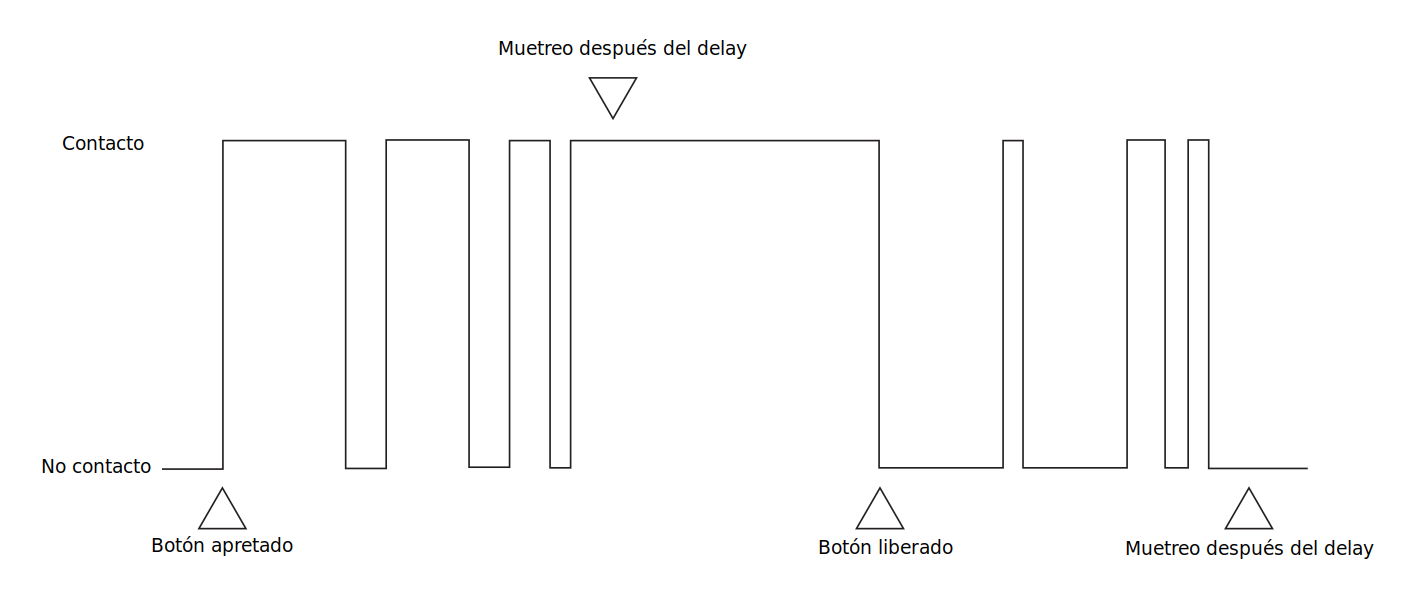
\includegraphics[width=0.9\linewidth]{antirebote.png}
    \caption{Ejemplo de señal de un botón siendo afectada por el fenómeno de rebote, extraída de \citep{douglass}.}
    \label{botonReboteD}
\end{figure}

En el libro de Douglass \cite{douglass} encontramos una propuesta de solución más cerca de la implementación que del diseño, algo así como un patron idiomático. En el Código \ref{deboun} se puede ver un extracto del libro, en donde se muestra la función que lleva a cabo la solución del autor. Esta consiste en utilizar un temporizador para permitir un tiempo de gracia antes de confirmar una transición en el estado. Esto es, al percibir un cambio en la entrada se inicia el \textit{timer} y se confirma el cambio de estado solo si el valor de la entrada sigue siendo distinto que antes de percibir la modificación. 

\begin{lstlisting}[caption=Código ejemplo de una estrategia de deteccion de rebote extraído de \cite{douglass}.,label=deboun]
void ButtonDriver_eventReceive(ButtonDriver* const me) {
    Timer_delay(me->itsTimer, DEBOUNCE_TIME);
    if (Button_getState(me->itsButton) != me->oldState) {
        /* must be a valid button event */
        
        me->oldState = me->itsButton->deviceState;
        
        if (!me->oldState) {
            
            /* must be a button release, so update toggle value */
            if (me->toggleOn) {
                me->toggleOn = 0; /* toggle it off */
                Button_backlight(me->itsButton, 0);
                MicrowaveEmitter_stopEmitting(me->itsMicrowaveEmitter);
            }
            else {
                me->toggleOn = 1; /* toggle it on */
                Button_backlight(me->itsButton, 1);
                MicrowaveEmitter_startEmitting(me->itsMicrowaveEmitter);
            }
        }
        /* if it’s not a button release, then it must
        be a button push, which we ignore.
        */
    }
}
\end{lstlisting}

Desde el punto de vista de la \gls{IS}, podemos decir que se está aplicando una mala práctica si queremos anticiparnos al cambio. El estado del botón se almacena en una variable y las funciones modifican su comportamiento mediante sentencias \textit{if}. Como vimos en el Capítulo \ref{cap:state}, este enfoque puede conllevar múltiples inconvenientes al momento de expandir o modificar los estados. Si se debe agregar uno nuevo, todas las sentencias \textit{if} deben actualizarse, lo que implica modificar la implementación de, en este caso, la función \verb|ButtonDriver_eventReceive|.

Una solución más alineada con los principios de la \gls{IS} consiste en aplicar el patrón de diseño \textit{State} \ref{anexoState} de Gamma, como vimos en el Capítulo \ref{cap:state}. Podemos identificar dos estados principales: \textit{On} y \textit{Off}. Sin embargo, como veremos más adelante, será necesario añadir dos estados adicionales para poder representar el comportamiento deseado.

Volviendo al ejemplo del libro, ante la detección de actividad en el botón se recibe un evento. A continuación, se da un tiempo de gracia y luego se vuelve a verificar el valor que adopta la señal proveniente del botón en el registro. Este valor determina si la señal indica que el botón está encendido o no. Haciendo uso de estos recursos, utilizaremos el patrón \textit{State} para representar cuatro posibles estados: \textit{On}, \textit{Off}, \textit{OnWait} y \textit{OffWait}. Los dos primeros reflejan que el botón se encuentra encendido o apagado, respectivamente, mientras que los otros dos corresponden a la etapa de espera durante el tiempo de gracia, necesaria para determinar si existió o no una transición. Esta máquina de estados es la definida en la Figura \ref{maquinaBoton}.

\begin{figure}[H]
\caption{Máquina de estados propuesta para el control antirebote.}
\label{maquinaBoton}
\begin{center}
\scalebox{.90}{
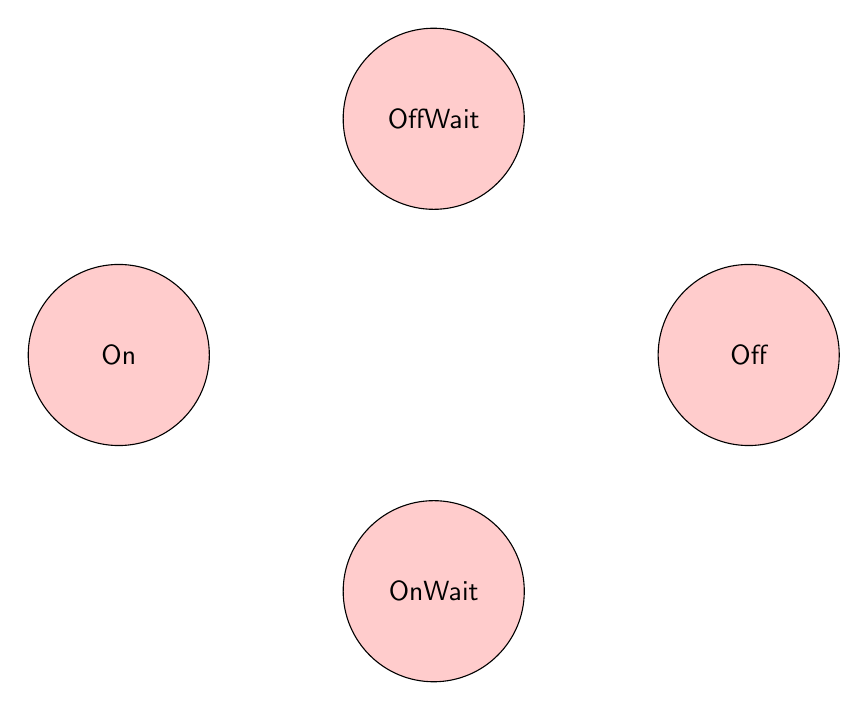
\begin{tikzpicture}[umlstate/.style={
    circle,
    draw,
    minimum size=2.3cm,
    fill=red!20,
    font=\sffamily
}]

\node[umlstate] (On) at (-4,0) {On};
\node[umlstate] (Off) at (4,0) {Off};
\node[umlstate] (OnWait) at (0,3) {OffWait};
\node[umlstate] (OffWait) at (0,-3) {OnWait};

\umltrans[arg=evento, pos=0.5, anchor1=60, anchor2=-160] {On}{OnWait}
\umltrans[arg=time, pos=0.5, anchor1=-125, anchor2=25] {OnWait}{On}
\umltrans[arg=time, pos=0.5] {OnWait}{Off}
\umltrans[arg=evento, pos=0.5, anchor1=-125, anchor2=25] {Off}{OffWait}
\umltrans[arg=time, pos=0.5, anchor1=60, anchor2=-160] {OffWait}{Off}
\umltrans[arg=time, pos=0.5] {OffWait}{On}


\end{tikzpicture}
}
\end{center}
\end{figure}

\declareCMod{Temporizador}

Por otro lado, para gestionar el tiempo de gracia utilizaremos un módulo llamado \Temporizador, el cual permite suscribir un método que será invocado luego de transcurridos \textit{x} segundos. Todos estos módulos pueden observarse en el diagrama de la Figura \ref{modulosBoton}.

\begin{figure}[H]
\caption{Módulos encargados de gestionar el comportamiento del temporizador utilizado en la transiscion de estados del módulo Boton.}
\label{modulosBoton}
\begin{center}
\scalebox{.90}{
\begin{tikzpicture}\sf

\umlclass[]{Temporizador}
{}
{
setTiempo(i: Real) \\
start() \\
}

\umlnote[above right=-1cm and 1cm of Temporizador,width=5cm]{Temporizador}{
tickHandler() \{ \\
\ \ \ \ botonTime.execute() \\
\}
}


\umlsimpleclass[below right=-1cm and 3cm of Temporizador]{BotonTime}
\umluniassoc[arg1=botonTime,pos1=0.5,anchor1=-18]{Temporizador}{BotonTime}
\umlnote[below=1cm of BotonTime,width=5cm]{BotonTime}{
execute() \{ \\
\ \ \ \ boton.time() \\
\}
}


\end{tikzpicture}
}
\end{center}
\end{figure}

\declareCMod{Boton}

Resuelto el funcionamiento del temporizador, veamos ahora el módulo \Boton, que será el utilizado por los clientes para conocer el estado del botón físico. Para ello, definimos también el estado y el módulo que encapsula el acceso al registro donde se almacena el valor de la señal proveniente del botón. Todos estos módulos pueden observarse en la Figura \ref{botonCompleto}.


\begin{figure}[H]
\caption{Diagrama de módulos relacionados al boton.}
\label{botonCompleto}
\begin{center}
\scalebox{.90}{
\begin{tikzpicture}\sf

\umlclass[x=-4]{Boton}
{}
{prendido(): Bool\\
evento() \\
time() \\
changeState(i: EstadoBoton)
}

\umlclass[right=2cm of EstadoBoton,type=abstract]{EstadoBoton}
{}
{
\umlvirt{prendido()} \\
\umlvirt{evento(i: Boton)} \\
\umlvirt{time(i: Boton)} \\

}

\umlclass[below left=2cm and 1cm of EstadoBoton]{On}
{}
{
...
}


\umlclass[below left=2cm and -1.5cm of EstadoBoton]{Off}
{}
{
...
}

\umlclass[below right=2cm and -1.5cm of EstadoBoton]{WaitOn}
{}
{
...
}

\umlclass[below right=2cm and 1cm of EstadoBoton]{WaitOff}
{}
{
...
}

\umlclass[above=1cm of EstadoBoton]{RegistroBoton}
{}
{
getValor(): Bool
}

\umlnote[below left=1cm and -5cm of Boton, width=4.5cm]{Boton}{
prendido() \{\\
\ \ \ \ return st.prendido() \\
\}\\
\\
\rule{0.5\linewidth}{0.3pt}\\
\vspace{1mm}
evento() \{\\
\ \ \ \ return st.evento(this) \\
\}\\
\\
\rule{0.5\linewidth}{0.3pt}\\
\vspace{1mm}
time() \{\\
\ \ \ \ return st.time(this) \\
\}\\

}

\umlnote[below=3cm of On, width=5cm]{On}{
evento(Boton b)\{\\
\ \ \ \ timer.start() \\
\ \ \ \ b.changeState(WaitOff) \\
\}\\
\rule{0.5\linewidth}{0.3pt}\\
\vspace{1mm}
prendido()\{\\
\ \ \ \ return True\\
\}
}

\umlnote[below left=1cm and -2cm of WaitOff, width=5cm]{WaitOff}{
evento(Boton b)\{\\
\ \ \ \ return \\
\}\\
\\
\rule{0.5\linewidth}{0.3pt}\\
\vspace{1mm}
time(Boton b)\{\\
if not registro.getValor()\{ \\
\ \ \ \ b.changeState(Off)\\
\}else\{\\
\ \ \ \ b.changeState(On)\\
\}\\
\\
\rule{0.5\linewidth}{0.3pt}\\
\vspace{1mm}
prendido()\{\\
\ \ \ \ return True\\
\}
}


\umlinherit[geometry=|-|]{On}{EstadoBoton}
\umlinherit[geometry=|-|]{Off}{EstadoBoton}
\umlinherit[geometry=|-|]{WaitOn}{EstadoBoton}
\umlinherit[geometry=|-|]{WaitOff}{EstadoBoton}
\umluniaggreg[geometry=-|-,arg1=st, pos1=0.5]{Boton}{EstadoBoton}


\end{tikzpicture}
}
\end{center}
\end{figure}

\declareCMod{On}
\declareCMod{Of}
\declareCMod{OnWait}
\declareCMod{OffWait}

Repasemos cómo funciona el sistema con la estructura propuesta. Supongamos que el botón se encuentra encendido, por lo tanto, su estado es \On. Cuando se produce un evento, es decir, se detecta algún tipo de cambio en la señal proveniente del botón, se ejecuta el método \verb|evento| del módulo \Boton. Este último delega su funcionamiento al estado. Como dijimos que el botón estaba prendido, el encargado de manejar el evento será \On. Este iniciará el temporizador con el tiempo configurado y cambiará el estado del módulo \Boton a \WaitOff. Estando el botón encendido, solo puede apagarse; es por eso que se transiciona al estado \WaitOff, el cual decidirá, una vez transcurrido cierto tiempo, si corresponde pasar a \Off. Esto lo hace verificando el valor presente en el registro del botón cuando el temporizador ejecuta el método \verb|time()| de \Boton. En caso de que el registro muestre que el botón está apagado, efectivamente se cambiará el estado a \Off; en caso contrario, se volverá a \On, ya que se trató de una detección errónea, probablemente provocada por el efecto rebote. 

Todos los estados deben implementar el método \verb|prendido():Bool|, que es el utilizado por los clientes para conocer el verdadero estado del botón. Si el estado es \On o \WaitOff, \verb|prendido():Bool| devolverá \verb|True|; en caso contrario, devolverá \verb|False|.

Dado que la solución propuesta es una aplicación del patrón \textit{State}, debe ser documentada con el método 2MIL, tal como se presenta en la sección \ref{docDeboun}.

\begin{figure}
\caption{Documentacion de la aplicación del patrón State para el control del estado del botón.}
\label{docDeboun}
\scalebox{.90}{
\begin{pattern}[]{Estados del botón}{Algorithm}{idFigAlg}
\based{Estado (State)}
\why{\textbf{Cambios previstos}: Pueden mofificarse los estados de cotrol del botón en base a nuevos requerimientos o cambios en el hardware.

\textbf{Funcionalidad}: La interfaz de usuario mostrará el botón como encendido o apagado según su estado interno. Para crear un retardo en las transiciones, es necesario añadir estados intermedios que gestionen esa demora.
}
\assigns
\is{Boton}{Contexto}
\is{EstadoBoton}{Estado}
\is{On}{EstadoConcreto}
\is{Off}{EstadoConcreto}
\is{OnWaiting}{EstadoConcreto}
\is{OffWaiting}{EstadoConcreto}
\end{pattern}
}
\end{figure}


De esta manera, logramos encapsular cada estado en un módulo independiente, que puede ser modificado sin afectar al resto. Además, agregar nuevos estados resulta sencillo: basta con crear un nuevo módulo.



\section{Verificación de precondiciones}
El autor del libro \cite{douglass} comenta que uno de los problemas más grandes que observa en el desarrollo de sistemas embebidos es que muchas funciones tiene precondiciones para ejecutarse correctamente, pero que rara vez se verifica que todas se cumplan. Además, el procedimiento común de informar precondiciones inadecuadas en una función en \textbf{C}\footnote{Lenguaje de programación comúnmente utilizado en sistemas embebidos.} es a través del valor de retorno (-1 en caso de errores, 0 en el contrario). Por lo tanto, el encargado de manejar el error es la función que invocó a la segunda, generando así un acoplamiento extra en el código. Esto provoca una complicación que muchas veces deriva en un mal manejo de los errores. Por ejemplo, supongamos que se tiene un módulo que exporta un método que realiza cierto cómputo en base a dos argumentos, \verb|computar(i: int, i: int)|. Existen múltiples posibles implementaciones, estas son algunas:
\begin{itemize}
    \item Una posible implementación consiste en que la función no realice ninguna verificación y simplemente intente utilizar los valores pasados como argumento, lo cual puede generar un error inmediato si los tipos no coinciden, o un error futuro si el valor está fuera de los parámetros requeridos por el sistema. Por ejemplo, si se pasa un entero negativo, pero el método requiere como precondición que siempre sea positivo, se podría provocar un error división por cero más adelante en la ejecución; esta implementación obliga a que todos los clientes que utilicen este método deban verificar la validez de los valores, lo que no solo genera código repetido, sino que también requiere una actualización manual en múltiples puntos si el requisito cambia, haciendo que la responsabilidad de la verificación de las precondiciones recaiga en el cliente que utiliza la función, en lugar de ser manejada internamente por la misma.
    \item Otra opción se basa en verificar si el valor es permitido, haciendo que \\ \verb|computar(i: int, i: int)| retorne un valor que indique el resultado de la validación (por ejemplo, 0 en caso afirmativo y -1 en caso contrario). Si bien este enfoque es una mejora respecto a no realizar validación alguna, continua con el acoplamiento entre el cliente de la función y el módulo que la exporta, ya que el cliente debe verificar el valor de retorno para determinar si ha ocurrido un error.
\end{itemize}

La solución propuesta en el libro de Douglass \cite{douglass} es más cercana a un patrón idiomático o a una práctica de programación que a un patrón de diseño. Sus conceptos clave son los siguientes:

\begin{itemize}
    \item Construir tipos de autoverificación siempre que sea posible.
    \item Verificar los valores de los parámetros entrantes para un rango adecuado.
    \item Verificar la consistencia y razonabilidad entre uno o un conjunto de parámetros.
\end{itemize}

Por lo tanto, la solución planteada no constituye un patrón de diseño general. No obstante, desde la perspectiva de la \gls{IS}, es posible preparar el sistema para futuros cambios y, al mismo tiempo, realizar las verificaciones necesarias. Para ello, proponemos la aplicación del patrón \textit{Decorator} \ref{anexoDecorator} de Gamma, el cual permite añadir o eliminar funcionalidades a módulos de manera dinámica. En particular, lo que se busca es agregar la verificación de cada argumento, manteniéndola separada del módulo que implementa la funcionalidad específica.

\declareCMod{ErrorHandler}

Para la construcción de la solución, se tomará del libro \cite{douglass} el concepto de un módulo denominado \ErrorHandler, o manejador de errores. Esta es una técnica ampliamente utilizada e incorporada en ciertos lenguajes de programación, que se basa en delegar la gestión de un error a un módulo especializado. Dicho módulo, basándose en la lógica definida por el desarrollador, resolverá el inconveniente; por ejemplo, puede mostrar un error en pantalla y detener la ejecución, reintentar ejecutar un método o reiniciar ciertos componentes. Existen múltiples enfoques para este problema, algunos de los cuales se estudian en \cite{glass2009graceful}.

Lo relevante de esta estrategia es que el módulo proporciona una interfaz clara para el manejo de errores, cuya estructura se detallará a continuación con un ejemplo.

\declareAMod{Mecanismo}
\declareCMod{MecanismoConcreto}


Suponga que se tiene el módulo \Mecanismo cuya interfaz es la que se muestra en la Figura \ref{mecanismo}. Como se puede ver uno de los métodos es \verb|computar|, el cual para funcionar correctamente y sin errores, requiere que el primer argumento sea siempre mayor a cero y que el segundo sea par. En lugar de agregar el Código \ref{verificacion} al inicio de la implementación de \verb|computar|, proponemos usar dos módulos que actúen como decoradores y encapsulen esta funcionalidad.


\begin{figure}[H]
\caption{Interfaz del módulo Mecanismo.}
\label{mecanismo}
\begin{center}
\scalebox{.90}{
\begin{tikzpicture}\sf

\umlclass[type=abstract]{Mecanismo}
{}
{
...\\
\umlvirt{computar(i: int, i: int)}\\
...\\
}
\end{tikzpicture}
}
\end{center}
\end{figure}

\begin{lstlisting}[caption=Verificación de precondiciones en método Computar.,label=verificacion]
computar(int primer, int segundo){
	if (primer <= 0)
		return -1
	if (segundo % 2 != 0)
		return -1
	.
	.
	.
\end{lstlisting}

En la Figura \ref{estructuraDeco} se presenta la estructura de módulos conseguida a partir de la aplicando el patrón y el uso del módulo \ErrorHandler.

\begin{figure}[H]
\caption{Ejemplo de aplicación del patrón \textit{Decorator} \ref{anexoDecorator} para garantizar el cumplimiento de precondiciones.}
\label{estructuraDeco}
\begin{center}
\scalebox{.90}{
\begin{tikzpicture}\sf
\umlclass[type=abstract]{Mecanismo}{}
{
\umlvirt{...}\\
\umlvirt{computar(i: int, i: int)}\\
\umlvirt{...}
}

\umlclass[below left=2cm and -1cm of Mecanismo]{MecanismoConcreto}{}
{
...\\
computar(i: int, i: int)\\
...\\
}

\umlclass[below right=2cm and -1cm of Mecanismo,type=abstract]{Decorador}{}
{
\umlvirt{...}\\
\umlvirt{computar(i: int, i: int)}\\
\umlvirt{...}
}

\umlclass[below right=1.5cm and -1.5cm of Decorador]{SegundoArgPar}{}
{
...\\
computar(i: int, i: int)\\
...\\
}

\umlclass[below left=1.5cm and -1.5cm of Decorador]{PrimerArgPositivo}
{
}
{
...\\
computar(i: int, i: int)\\
...\\
}



\umlinherit[geometry=|-|]{MecanismoConcreto}{Mecanismo}
\umlinherit[geometry=|-|]{Decorador}{Mecanismo}
\umlinherit[geometry=|-|]{PrimerArgPositivo}{Decorador}
\umlinherit[geometry=|-|]{SegundoArgPar}{Decorador}
\umluniaggreg[geometry=-|-,arm1=2cm,anchor1=east,anchor2=east,arg1=mecanismo,
pos1=0.5]{Decorador}{Mecanismo}

\umlnote[below left= 1cm and -2cm of SegundoArgPar,width=8cm, geometry=-|,anchor2=-60]{SegundoArgPar}{
computar(primero, segundo)\{ \\
if (segundo \% 2 != 0)\{\\
\ \ \ \	errorHandler.manejarError(error de argumento)\\
\}else\{\\
\ \ \ \	return mecanismo.computar(primero, segundo)\\
\}\\
}

\umlclass[left=1cm of PrimerArgPositivo]{ErrorHandler}
{
}
{
    manejarError(i: Error)
}
\umluniassoc[geometry=|-|,anchor1=south,anchor2=south,arm1=-0.6cm]{SegundoArgPar}{ErrorHandler}
\umluniassoc{PrimerArgPositivo}{ErrorHandler}


\end{tikzpicture}
}
\end{center}
\end{figure}
\declareCMod{PrimerArgPositivo}
\declareCMod{SegundoArgPar}


Para utilizar el método \verb|computar| del módulo \MecanismoConcreto con la verificación de cada argumento, es necesario componerlo, en tiempo de ejecución, con todas las verificaciones de precondiciones deseadas; en este caso, \PrimerArgPositivo y \SegundoArgPar. De esta manera, el cliente ejecutará el método \verb|computar| de \PrimerArgPositivo, el cual realizará su verificación y, si es correcta, invocará el método computar del \Mecanismo que tiene compuesto, que en este caso es \SegundoArgPar. Este último hará lo mismo, pero invocando a \verb|computar| de \MecanismoConcreto. Así, se crea un encadenamiento de módulos de forma dinámica, lo que permite agregar y quitar funcionalidades con facilidad.

En la solución aplicamos un patrón de diseño, por lo tanto, debemos presentar la correspondiente documentación para que otros desarrolladores puedan comprender el diseño. Esta la podemos ver en la Figura \ref{docDecorator}.

\begin{figure}[H]
\caption{Documentación de la aplicación del patrón \textit{Decorator} al caso de verificación de la integridad de la información.}
\label{docDecorator}
\scalebox{.90}{
\begin{pattern}[]{Módulo decorador que extiende dinámicamente las funcionalidades de otro módulo sin cambiar la implementación.}{Algorithm}{idFigAlg}
\based{Decorador (Decorator)}
\why{\textbf{Cambios previstos}: Pueden agregarse y quitarse métodos de verificación u otras funcionalidades.

\textbf{Funcionalidad}: El módulo decorador es utilizado para extender la funcionalidad del módulo ComponenteConcreto. Antes de invocar al método de este último se ejecutan la homónima del decorador.
}
\assigns
\is{Mecanismo}{Componente}
\is{MecanismoConcreto}{ComponenteConcreto}
\is{Decorador}{Decorador}
\is{PrimerArgPositivo}{DecoradorConcreto}
\is{SegundoArgPar}{DecoradorConcreto}

\end{pattern}
}
\end{figure}

Con este diseño se añade una capa de verificación sin modificar el módulo original, lo que ofrece las siguientes ventajas:
\begin{itemize}
\item Se desacopla el cliente del módulo invocado, eliminando la necesidad de que el cliente verifique las precondiciones de un método antes de su ejecución.
\item La lógica de cada verificación se encapsula en un solo módulo, manteniendo la separación de responsabilidades y facilitando su reutilización. De esta forma, la implementación del módulo original que realiza el comportamiento requerido no necesita ser modificado.
\item El patrón \textit{decorador} permite que el sistema pueda evolucionar, permitiendo añadir nuevas funcionalidades o modificar las reglas de verificación sin afectar la implementación original. Esto hace posible, por ejemplo, implementar restricciones de acceso, límites en las operaciones sin alterar el módulo subyacente o verificaciones de integridad de la información mucho más complejas (ver Sección \ref{integridad} a continuación).
\end{itemize}

\subsection*{Integridad de la información}
\label{integridad}
\declareCMod{Data}

Como se ha señalado en otros \textit{problemas comunes}, el ejemplo propuesto es una versión simplificada, pero es posible agregar funcionalidades mucho más complejas. Una de ellas es la verificación de la integridad de la información almacenada en el sistema.

Douglass, en \cite{douglass}, sostiene que uno de los orígenes más comunes de inconvenientes relacionados con fallas de seguridad o confiabilidad es la corrupción de la información. Un pulso electromagnético o fallas en el hardware pueden causar daños en los datos, comprometiendo su integridad; por ejemplo, alterando un \gls{bit} o provocando la pérdida parcial de cierta zona de la memoria. Si los datos afectados son críticos, el problema puede derivar en un error grave del sistema. Para hacer frente a esto, existen diversas técnicas, desde el cálculo de checksums con el fin de verificar la integridad, hasta el almacenamiento de la información múltiples veces para crear redundancia.

Estas técnicas suelen ser añadidas al código modificando la implementación de los métodos del módulo encargado de almacenar la información, o agregando verificaciones en las partes del código que la utilizan. Es decir, si se utiliza el módulo \Data (ver Figura \ref{dataInter}), se realiza una llamada al método \verb|getData()| para obtener la información almacenada y luego se ejecutan las validaciones necesarias para verificar su integridad. Este enfoque, sin embargo, provoca código repetido en cada llamada a \verb|getData()| y alto acoplamiento entre módulos. Por lo que, ante cualquier cambio en el formato de los datos, la estrategia de validación utilizada podría dejar de ser aplicable, lo que obligaría a modificar múltiples partes del código.

\begin{figure}[H]
\caption{Interfaz del módulo Data.}
\label{dataInter}
\begin{center}
\begin{tikzpicture}\sf
\umlclass[]{Data}
{
value: Dato \\
}
{
    getData(): Dato \\
    setData(i: Dato) \\
}

\end{tikzpicture}
\end{center}
\end{figure}

Analizando el patrón \textit{decorator} \ref{anexoDecorator} aplicado a este \textit{problema común}, se puede intuir que es posible utilizarlo para agregar al módulo \Data la funcionalidad de verificar la integridad de la información almacenada. La solución consiste en crear un decorador para el módulo \Data que, en primer lugar, obtenga la información y luego aplique algún tipo de verificación de integridad, como el cálculo de un \gls{checksum}. En el código \ref{getData} se puede observar una posible implementación de los métodos \verb|getData()| y \verb|setData()| de este nuevo decorador, siguiendo el procedimiento mencionado.

\begin{lstlisting}[caption=Implementación de los métodos getData y setData del decorador que se encarga de verificar la integridad de la información almacenada en el módulo \Data.,label={getData}]
setData(Dato i){
    this.checksum = calcularChecksum(i)
    data.setData(dato)
}

getData() {
    dato = data.getData()
    if (calcularChecksum(dato) == this.checksum)
        return dato
    else
        errorHandler(error de integridad)
}
\end{lstlisting}

Este es otro ejemplo en el que el patrón \textit{decorator} permite la adicion de una funcionalidad a un módulo sin modificarlo.


\section{Organización de la ejecución}
\label{orgEjecucion}

En un sistema robótico embebido se suelen ejecutar múltiples tareas para lograr un cierto objetivo. Ya sea, si se eligió seguir un estilo arquitectónico del tipo ``Control de procesos''(recordar Sección \ref{arqControlProc}) o no. Por lo general se debe verificar información recibida a través de sensores y otras fuentes (comunicación serial, web, etc.), realizar cómputos y efectuar acciones con los actuadores presentes en el sistema en tiempo real.

Una implementación simple para realizar el comportamiento mencionado, consiste en crear funciones para cada parte del proceso y llamarlas en \textit{loop} desde la función \textit{main}, y si es necesario añadir un tiempo de espera entre cada ejecución mediante \textit{sleeps}. La principal desventaja que conlleva este enfoque es que los sistemas robóticos son en tiempo real, es decir, por ejemplo se pueden perder \textit{inputs} de sensores si no se los maneja de manera correcta. Además, los tiempos de espera son bloqueantes por lo que se desperdicia acceso a cómputo.

Una estrategia para mejorar estos puntos consiste en utilizar las interrupciones del microcontrolador, lo que permite atender a todas las señales de entrada y a los eventos del entorno en tiempo real. En particular, en el diseño del robot desmalezador \cite{paperPomponio}, las interrupciones se utilizan en conjunto con un estilo arquitectónico de control de procesos \ref{arqControlProc}. El sistema resultante posee tres tareas principales:

\begin{itemize}
    \item Recibir información de los sensores y de la PC (por ejemplo, a través del puerto serial).
    \item Procesar la información recibida y decidir que valores aplicar en los actuadores.
    \item Aplicar los nuevos valores a los actuadores. Notar que no es tan simple como configurar un número y dejar que actúe, en muchos casos se necesita un seguimiento durante el tiempo.
\end{itemize}

De las tareas que se tienen, dos deben ser llamadas por el sistema y la otra (recibir información) en muchos casos se dará en forma de interrupciones que el sistema debe atender. Ya se comentó de ese proceso en la sección \nameref{obtInfo}, solo es importante recordar que la estructura propuesta provee una interfaz la cual se puede invocar para obtener la información recibida de manera simple. Una vez resuelta esa cuestión ahora se deben atender las otras dos tareas, dado que se quieren hacer los ajustes cada determinado tiempo, se propone crear una nueva interrupción que sea disparada de manera periódica y que su manejador se encargue de realizar todo el proceso de control y cálculo. En el manejo de esa interrupción, se accederá a las interfaces propuestas para obtener información de los sensores. Y por último, para los actuadores que necesitan un seguimiento temporal para su control, se agrega una nueva interrupción que puede ser individual para el actuador y el tiempo de disparo puede estar determinado de manera particular.

Como se puede deducir, el uso de interrupciones es abundante en sistemas de tiempo real y de control. Por lo tanto, resulta imprescindible tener un buen manejo de ellas. Las interrupciones, como su nombre indica, detienen la ejecución normal de un programa para atender a un evento. Una vez que este manejo finaliza, la ejecución continúa en el punto donde fue interrumpida (más información referida a interrupciones en la Sección \ref{secInterrupciones}).

Cuando una interrupción es interrumpida por otra, el sistema prioriza la más reciente, ejecutándola primero y reanudando después las anteriores. Un problema común y evitable surge con las interrupciones periódicas: si el tiempo de manejo de una interrupción es mayor que el intervalo de su disparo, por ejemplo, si un temporizador la genera cada \textit{x} segundos, pero su manejo tarda \textit{x} + 2 segundos, se produce una situación en la que la ejecución nunca finaliza hasta que se desactive el \textit{timer} que lanza las interrupciones. Además de que la tarea no se complete, el sistema puede quedar en un estado inconsistente. Por ejemplo, en un ciclo de control (lectura, procesamiento y actuación), una nueva interrupción puede ocurrir antes de que el ciclo concluya, provocando que la etapa de actuación sobre los actuadores nunca se ejecute y el sistema no realice ninguna acción.

Los problemas de concurrencia de este tipo son difíciles de detectar y corregir, por lo que es útil contar con herramientas para evitarlos. Una forma común de hacerlo es apagando las interrupciones del \gls{MCU} al comenzar el manejo de una interrupción. No obstante, esto no es ideal, ya que se perderían interrupciones no periódicas que sí se desean manejar. Otra opción es eliminar o desuscribir el manejador de la interrupción al comenzar su ejecución, aunque es crucial recordar volver a agregarlo para que el próximo ciclo se ejecute.

Desde la \gls{IS}, resulta interesante proponer un diseño para evitar este problema. Para ello, se aplicará el patrón \textit{State} \ref{anexoState} para representar dos estados posibles en relación con el manejo de una interrupción: \textbf{Activo} (disponible para manejar la interrupción) e \textbf{Ignorar} (el estado responsable de ignorar interrupciones mientras una está siendo manejada). De este modo, cuando el manejo de una interrupción comience, el estado cambiará a \textbf{Ignorar}, lo que hará que cualquier nueva llamada al manejador resulte en un retorno rápido. Una vez que la ejecución del manejo finalice, el estado volverá a cambiar, permitiendo el manejo de nuevas llamadas a la interrupción.

Veamos ahora la estructura de módulos subyacente a esta solución en la Figura \ref{estructuraInterrup} y en la Figura \ref{docStateInt} la correspondiente documentación del uso del patrón en este ejemplo.

\begin{figure}[H]
\caption{Ejemplo de manejador de interrupciones usando \textit{State} para prevenir inconvenientes en la ejecución.}
\label{estructuraInterrup}
\begin{center}
\scalebox{.90}{
\begin{tikzpicture}\sf


\umlclass[type=abstract]{Estado}
{
}
{
    \umlvirt{manejarInt(i: Manejador)} \\
}

\umlclass[left=2cm of Estado]{Manejador}
{
}
{
    manejarInt() \\
    cambiarEstado(i: Estado)
}

\umlclass[below right=2cm and -2cm of Estado]{Ignorar}
{
}
{
    manejarInt(i: Manejador) \\
}

\umlclass[below left=2cm and -2cm of Estado]{Activo}
{
Activo(i: Ignorar)
}
{
    manejarInt(i: Manejador) \\
}

\umlnote[below left=1cm and -1.5cm of Ignorar,width=5cm]{Ignorar}{
manejarInt(Manejador m) \{ \\
\ \ \ \ return\\
\}
}

\umlnote[left=1.5cm of Activo,width=5cm]{Activo}{
manejarInt(Manejador m) \{ \\
\ \ \ \ m.cambiarEstado(ignorar)\\
\ \ \ \ \textit{...manejo normal o}\\
\ \ \ \ \textit{ejecución de comando...}\\
\ \ \ \ m.cambiarEstado(this) \\
\}
}


\umluniaggreg{Manejador}{Estado}
\umlinherit[geometry=|-|]{Ignorar}{Estado}
\umlinherit[geometry=|-|,arm1=2.165cm]{Activo}{Estado}



\end{tikzpicture}
}
\end{center}

\end{figure}

\begin{figure}
\caption{Documentación de la aplicación del patron \textit{State} para el ejemplo del manejador de interrupciones.}
\label{docStateInt}
\scalebox{.90}{
\begin{pattern}[]{Control de manejo de interrupciones}{Algorithm}{idFigAlg}
\based{State (Estado)}
\why{\textbf{Cambios previstos}: Agregar, quitar o editar estados de manejo de la interrupción.

\textbf{Funcionalidad}: Configura el estado actual de manejo de una interrupción a fin de que una interrupción no pause la ejecución de otra del mismo tipo.
}
\assigns
\is{Manejador}{Contexto}
\is{Estado}{Estado}
\is{Ignorar}{EstadoConcreto}
\is{Activo}{EstadoConcreto}

\end{pattern}
}
\end{figure}


Al aplicar el uso de interrupciones junto con patrones de diseño como \textit{State}, el sistema embebido de control robótico adquiere una estructura más robusta y mantenible. Se logran reducir el riesgo de problemas de concurrencia provocados por el manejo de interrupciones en tiempo real. Y le quita responsabilidades a los módulos que efectivamente hacen el manejo de la interrupción.



\section{Control en conjunto de dispositivos}
Muchas aplicaciones embebidas robóticas controlan \gls{actuadores} que deben trabajar en conjunto para lograr el efecto deseado. Por ejemplo, para conseguir mover de manera coordinada un brazo robótico con múltiples articulaciones, todos los motores deben trabajar a la par. De manera similar, el uso de propulsores en una nave espacial en tres dimensiones requiere que muchos de estos dispositivos actúen en el momento preciso y con la cantidad correcta de fuerza para lograr la estabilidad necesaria. En ambos casos existe comunicación entre todos los componentes, ya sea para encadenar la ejecución de ciertos movimientos o para avisar de restricciones. Esto no es tarea simple y requiere de muchas líneas de código, por lo que un diseño orientado al cambio resulta clave.

\subsection*{Enfoque de diseño tradicional}

Antes de pasar a explicar la solución preparada para el cambio y analizar cómo aplicarla al ejemplo presentado por Douglass en su libro \cite{douglass}, se describirá cómo se aborda tradicionalmente esta problemática. Para ello, se tomará como ejemplo el software desarrollado para el robot desmalezador creado en conjunto por ingenieros electrónicos como parte del trabajo final de carrera \cite{disenioViejo1, disenioViejo2}. Los requerimientos son similares a los que se consideraron para el desarrollo del nuevo diseño orientado al cambio en \cite{paperPomponio}.

\subsubsection*{Estructura y funcionamiento general}

El sistema desarrollado controla el siguiente hardware del robot. Se cuenta con cuatro ruedas y un dispositivo de dirección que les permite girar. Cada rueda tiene sensores \gls{hall}, que permiten medir su posición y velocidad, y un sistema asociado de medición de corriente. El dispositivo de dirección permite determinar su posición angular en cada momento. Tanto las ruedas como el dispositivo de dirección pueden ser operados de forma remota mediante un control remoto (RC), capaz de enviar señales de dirección y velocidad a un módulo receptor de radiofrecuencia (RF) situado en el robot. Además, una computadora (PC) situada en el robot envía órdenes al dispositivo de dirección y a las ruedas para la navegación autónoma del robot. Las órdenes provenientes tanto del RC como de la PC son procesadas por un microcontrolador ubicado en el robot.

El código que conforma este sistema de control se encuentra dividido en unos pocos archivos, concentrando todo el flujo de control en \verb|main.c|, el resto contienen métodos que son invocados desde este último y proveen utilidades. No se utiliza programación orientada a objetos, en cambio, como estructura de organización del código se utilizan las funciones clásicas de C. Estas agrupan operaciones específicas como:
\begin{itemize}
\item Configuración de hardware.
\item Lectura de entradas (sensores, botones, etc.).
\item Control de salidas (motores, luces, etc.).
\end{itemize}

La información común entre muchas funciones se almacena en variables globales definidas en el mismo archivo. Entre las variables, encontramos algunas que se encargan de almacenar información referida al estado de operación del sistema. Es decir, que los estados se manejan con sentencias \verb|if| o \verb|switch case| (se comenta sobre esta solución en la Sección \nameref{cap:state}).

La función principal del sistema es \verb|main|, la misma se encarga de inicializar y calibrar los sensores y actuadores, de realizar el ciclo de control (recordar \ref{sistControl}) y terminar la ejecución. Para las primeras dos tareas llama a dos funciones que realizan el trabajo. El ciclo de control se ve representado por un bucle infinito en el cual se realizan las siguientes tareas principales:
\begin{itemize}
\item Lectura de entradas, es decir, valores de referencia a alcanzar.
\item Lectura de información de los sensores, dirección, velocidad y corriente.
\item En base al estado de ejecución actual, se realizan ciertas tareas. Por ejemplo, en el estado \verb|DUTY_REMOTO|, cuando el sistema está recibiendo una orden a través del control remoto, se lleva a cabo el ciclo de control completo. Por otro lado, en el estado \verb|EMERGENCIA|, el robot debe detenerse, por lo que su comportamiento será diferente.
\item Se aplican cambios a los actuadores, el ciclo de trabajo (\gls{PWM}) de los motores y la dirección.
\end{itemize}

\subsubsection*{Observaciones}
El criterio de división del código parece ser funcional, tanto por el aspecto del código, como por la documentación adjunta en los informes \cite[pág. 78-85]{disenioViejo1}, \cite[pág. 110-149]{disenioViejo2}. El criterio de división funcional, se centra es describir la funcionalidad de cada método y para hacerlo se muestra su comportamiento utilizando diagramas de flujo como el de la Figura \ref{diagra}. 

\begin{figure}[h]
\caption{Diagrama de flujo que explica el comportamiento de la función emergency \cite[pág. 82]{disenioViejo1}.}
\label{diagra}
\begin{centering}
{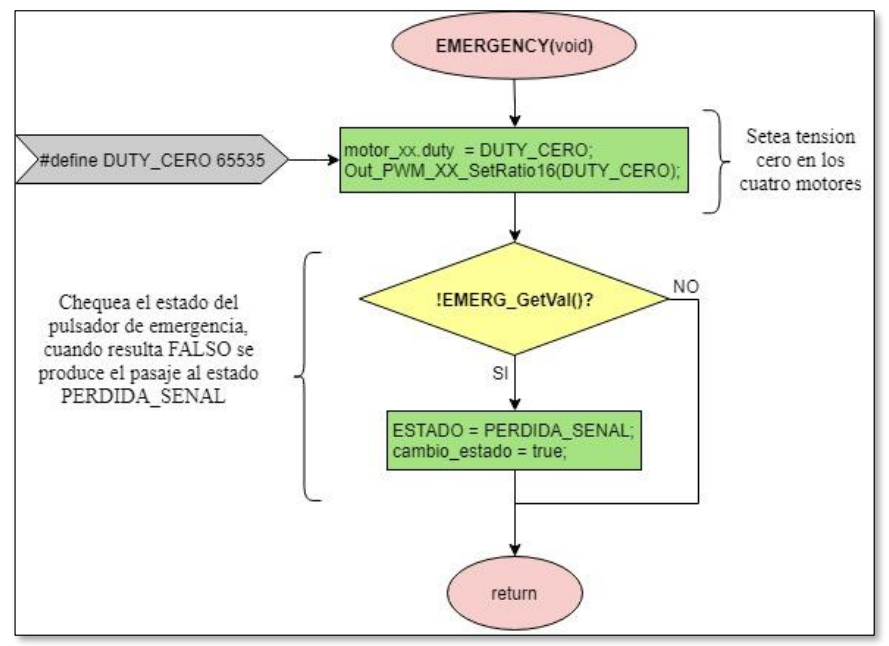
\includegraphics[width=0.8\textwidth]{diagramaFlujo.png}\par}
\end{centering}
\end{figure}


Por otro lado, a lo largo del código se utilizan estructuras condicionales (\textit{if, switch}, etc.) para determinar el flujo de ejecución. A su vez, las funciones que acceden directamente al hardware están integradas en la lógica del control (manejo del ciclo de control), lo que indica una baja separación entre la capa de abstracción del hardware y la gestión del ciclo de control. Esto es acompañado con un diseño procedimental, con una serie de pasos secuenciales y un control centralizado en el flujo principal \verb|main|.

Estos son otros inconvenientes referidos al cambio que están presentes en el código:
\begin{itemize}
\item El código parece estar compuesto por funciones largas y bloques monolíticos sin modularidad clara. Esto dificulta la localización y modificación de funcionalidades específicas, ya que los cambios pueden propagarse a otras partes del sistema que no son deseadas.
\item Los estados se definen en variables y se utilizan sentencias \textit{if} o \textit{switch} para cambiar el comportamiento de las funciones. Como se vio en la Sección \ref{cap:state} esto no es una buena práctica cuando se prepara el sistema para el cambio.
\item Hay valores ``hardcodeados'' (constantes definidas fijas en el código). Si estos valores cambian, es necesario modificar el código fuente, aumentando el riesgo de introducir errores. Además, se utilizan múltiples variables globales, las cuales añaden acoplamiento entre funciones y se debe ser cuidadoso al momento de introducir cambios que las afecten.
\item Las dependencias entre funciones están estrechamente acopladas. Lo que provoca que los cambios puedan requerir modificaciones significativas en diferentes secciones de código.
\item El manejo de errores parece ser inconsistente o inexistente en varias secciones. Es decir, no hay una decisión de diseño que contemple la existencia de posibles errores durante la ejecución. Esto puede llevar a comportamientos impredecibles y dificultar el diagnóstico de problemas.
\end{itemize}

\subsubsection*{Conclusión}

El diseño del código parece estar orientado a cumplir con un objetivo específico mediante un flujo procedimental y un control directo de los periféricos del hardware. Este enfoque es funcional, pero carece de modularidad y abstracción, lo que lo hace menos flexible y más difícil de mantener. La estructura no parece diseñada para escalar con nuevas funcionalidades.

\subsection*{Enfoque mejorado pero deficiente}

A continuación se describirá un ejemplo extraído de \cite[Sección. 3.4]{douglass}, se explicará la solución propuesta en el mismo libro para luego proponer una solución orientada al cambio.

\subsubsection*{Requisitos del sistema de control de un brazo robótico}
\label{requisitos}

Se necesita desarrollar el software de control de un brazo robótico que consta de tres \gls{actuadores}, dos \glspl{pasoapaso} (uno para rotar en su base y otro para extender o retraer el brazo) y una pinza que se puede cerrar o abrir. En le Figura \ref{brazoEsquema} podemos observar un esquema del hardware. Para controlar el comportamiento del brazo, se provee una función compleja la cual toma coordenadas en el espacio y devuelve una secuencia de pasos para que el brazo tome un objeto en la posición determinada por las coordenadas. Cada paso consta de una orden para cada actuador del brazo robótico. Estos se deben ejecutar de manera secuencial, es decir que el paso número dos empezará su ejecución solo si el primero culminó completamente y con éxito. En caso de que las coordenadas sean inalcanzables la función devuelve cero pasos. Si se produce un error durante la ejecución de un paso, se detiene la ejecución del sistema.

Controlar \glspl{pasoapaso} es más complejo de lo que parece. Habitualmente, se gestionan con dos funciones: una que define el sentido de giro y otra que ordena dar un solo paso. La longitud de cada paso viene determinada por el hardware del motor. Por lo tanto, para lograr movimientos más largos, se deben ejecutar múltiples pasos, lo que requiere un control exhaustivo por parte del software. Este es un requerimiento implícito que el sistema tiene y se deberá atender.

\begin{figure}[H]
\caption{Esquema del brazo robótico.}
\label{brazoEsquema}
\begin{centering}
{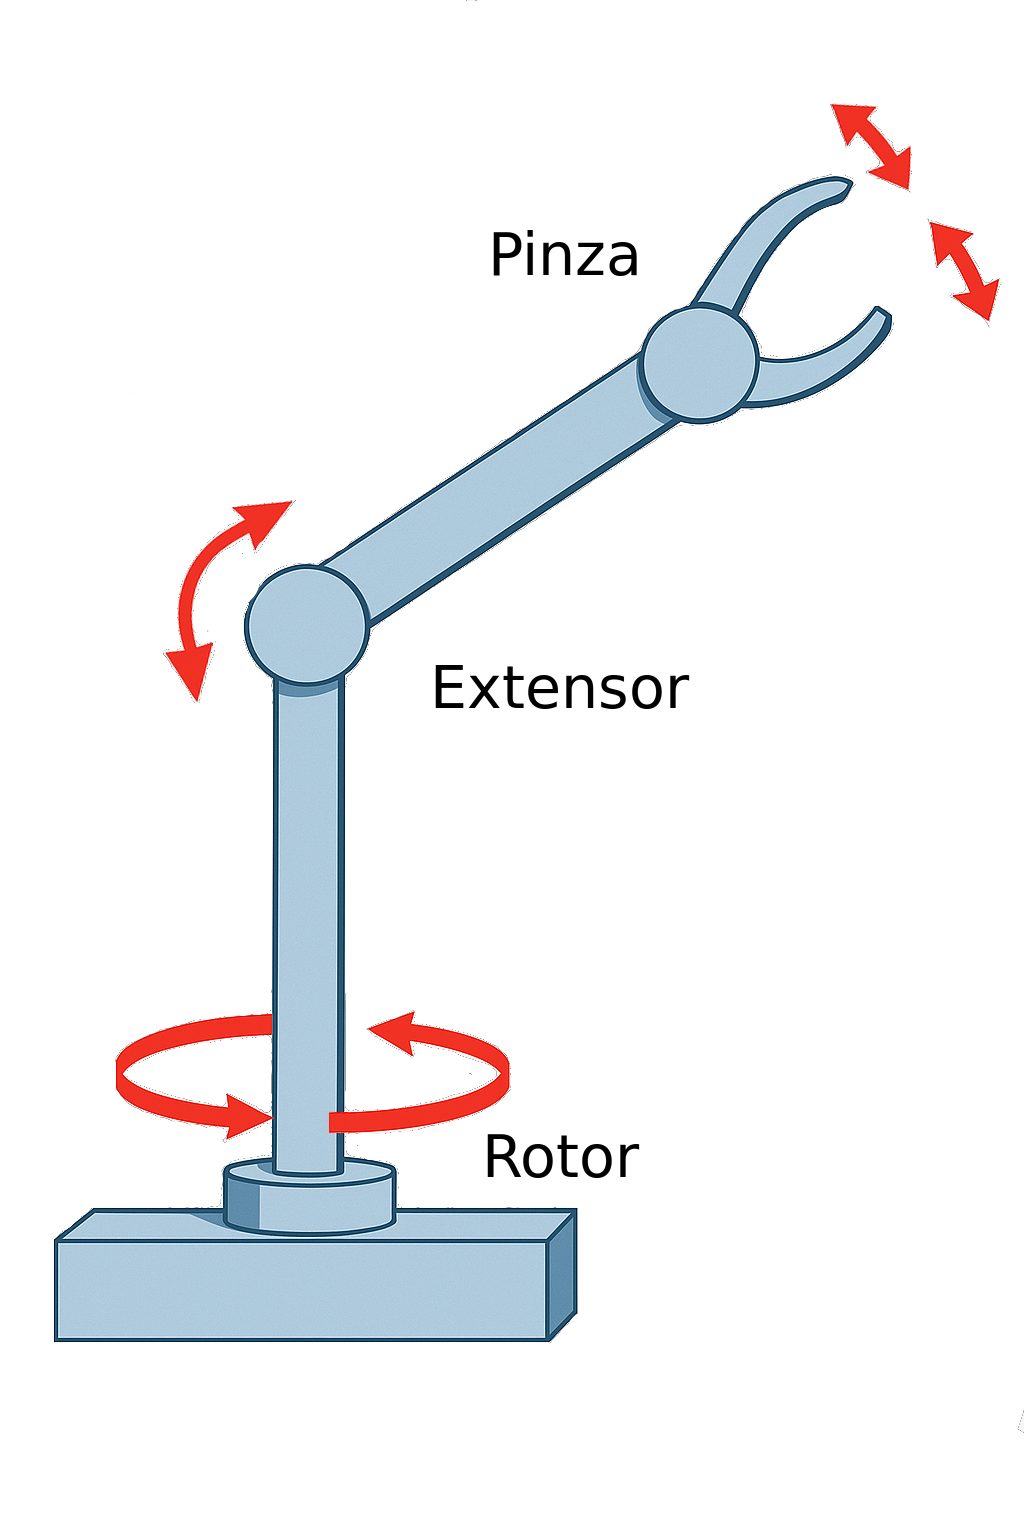
\includegraphics[width=0.4\textwidth]{brazo3.png}\par}
\end{centering}
\end{figure}

\subsubsection*{Solución propuesta en el libro de Douglass}

Como solución, el autor propone la creación de un módulo llamado \textbf{RobotArmManager}, cuya función es gestionar los actuadores y coordinar su comportamiento. Además, para cada tipo de actuador, se crea un módulo específico encargado de su control. Este módulo proporciona métodos para consultar el estado actual (posición, longitud, etc.) y otros para establecer un valor, similar a un \textit{set-point}. Dichos métodos desempeñan el rol de ejecutores de la acción, es decir, toman un valor \textit{set-point}, ejecutan la acción y retornan \verb|True| si fue satisfactoria, o \verb|False| en caso contrario.

El comportamiento del sistema comienza con la generación de una lista de pasos a realizar. Luego, se itera sobre esta lista ejecutando las acciones definidas en cada paso. Como el sistema debe interrumpir la ejecución si encuentra un error, el \textbf{RobotArmManager} verifica el valor de retorno tras cada acción. La ejecución de un movimiento completo finaliza cuando se completan todos los pasos generados previamente por la función que se mencionó en los requerimientos. En este caso es llamada \verb|graspAt(i: Coordenadas)|.

La solución propuesta parece estar un nivel de abstracción por encima de lo que se esperaría para este caso. Aunque no hay suficiente información sobre el hardware del brazo robótico, sabemos que utilizar \glspl{pasoapaso} no es tan simple como invocar un método. Este proceso suele requerir control continuo, operando mediante pulsos que hacen que el motor avance de a un paso. Por lo tanto, los módulos encargados de los movimientos probablemente tengan más responsabilidades de las que se plantean en el libro. Esto va en contra de las prácticas de la \gls{IS}, que establecen que un módulo debe ocultar un solo elemento de cambio. Además, sería necesario implementar un sistema de control más complejo, utilizando algún tipo de \textit{timer} o espera, para garantizar que el \gls{pasoapaso} tenga el tiempo necesario para actuar.

De todas formas, suponiendo que los módulos mencionados se adaptan al hardware subyacente, Douglass aplicar el patrón \textit{Mediator} \ref{anexoMediator} de Gamma. De manera que \textbf{RobotArmManager} cumple el rol de \textbf{Mediador} y cada módulo que se encarga de manejar cada actuador cumple el rol de \textbf{Colega}. Los autores en \cite{Gamma:1995:DPE:186897} establecen que el patrón es aplicable en los siguientes casos:
\begin{itemize}
\item Un conjunto de módulos se comunica de maneras bien definidas pero complejas. Las interdependencias resultantes son poco estructuradas y difíciles de comprender.

\item Reutilizar un módulo resulta complicado porque este se refiere y se comunica con muchos otros módulos.

\item Un comportamiento distribuido entre varios módulos debería ser personalizable sin requerir una gran cantidad de submódulos.
\end{itemize}

La estructura construida por Douglass es similar al patrón y logra el objetivo de reducir el acoplamiento entre colegas, evitando que los módulos se refieran directamente entre ellos. Podemos decir desde la perspectiva de la \gls{IS} que la aplicación del patrón ayuda a preparar el sistema ante un cambio en los colegas o su forma de comunicación.

Por otro lado, un ítem de cambio común son las estructuras de datos, como se mencionó en la Sección \ref{listaItems}. Por ello, establecer el uso de una lista directamente en la interfaz de un módulo no responde a una buena práctica.

Es posible que el problema haya sido simplificado con fines didácticos. Con el objetivo de explicar la aplicación del patrón \textit{Mediator}. La solución planteada parece alejarse de una implementación realista, dejando requisitos menos específicos que podrían dar lugar a diferentes interpretaciones.



\subsection*{Enfoque para el cambio: Subsistemas de control}
\label{subsistema}
\addcontentsline{toc}{subsection}{Subsistemas de control}

Para dar la solución orientada al cambio y completa que se propone en este trabajo, primero se introducirá el concepto de lo que llamaremos \textbf{Subsistema de control}. El cual fue extraído del trabajo realizado en el robot desmalezador \citep{paperPomponio} y se utilizará como diseño de referencia.

En un sistema complejo donde se controlan múltiples propiedades físicas, el sistema se divide en subsistemas. Cada subsistema controla \textbf{una} propiedad específica y se organiza según el estilo arquitectónico de control de procesos \ref{arqControlProc}. De esta manera, se logra independencia entre el control de cada propiedad, lo que prepara al sistema para cambios individuales en el control de cada una de ellas. Además, se promueve la reutilización del código, ya que un subsistema de control diseñado para manejar una propiedad específica puede aplicarse en diferentes escenarios o sistemas.

Estos subsistemas de control son una estructura de módulos relacionados mediante herencia, composición o invocación. Cuyo trabajo es lograr que cierta propiedad física alcance el valor deseado. Para hacerlo interactúa con la variable a manipular y las variables medidas relacionadas (recordar Tabla \ref{tab:conceptosArq}). En la Figura \ref{modulosSub} se puede observar de manera concreta los módulos que forman parte de cada componente de un subsistema. Para permitir la interacción con un cliente externo deben proveer una interfaz que permita establecer un valor al que se quiera llevar la propiedad (ver \textit{setPoint} en la Tabla \ref{tab:conceptosArq}) y que indique el comienzo de la tarea de control.

\begin{figure}[H]
\caption{Módulos de un subsistema de control y el componente arquitectónico al que pertenecen.}
\label{modulosSub}
\begin{center}
\begin{tikzpicture}\sf

\tikzstyle{moduloL}=[minimum width=3cm, minimum height=1.5cm,inner sep=2mm,above right,draw,align=center, font=\scshape] 

\tikzstyle{supest}=[rounded corners=1.5mm, minimum width=2cm,inner sep=2mm,draw,text width=2cm]

\tikzstyle{nombre}=[inner sep=0mm, font=\bfseries]

\tikzstyle{pipe}=[-latex,thick,line width=4pt]

\tikzstyle{nombreLogico}=[inner sep=0mm, font=\scshape, minimum width=1.5cm]

%---figura control-----
\tikzstyle{ctrl}=[shape=circle,draw,minimum width=2.5cm,text width=2cm, inner sep=2, align=center,font=\scshape];


%----figura de sensor---
\tikzstyle{sensor}=[draw,circle, minimum width=1cm,after node path={(\tikzlastnode) circle (0.2cm)}]
% se usa así: \draw node[sensor]{};

%---------------------------------------
%---control del proceso rueda----
\node[ctrl, text width=1.8cm] (0,0) (controlR){Control};
%
\node[moduloL, below=2cm of controlR, minimum width=3cm](procesoArq){Proceso};
%%
\draw node[sensor, below=2cm of procesoArq](sensorCte){};
%%
%%%puntos para hacer las flechas de las señales hacia los sensores
\node[below=4.5cm of procesoArq](pto2){};
%%
\draw[dashed, -latex](procesoArq)--(pto2);
%%
\node[nombreLogico, below left=-0.1cm and 0.1cm of sensorCte, text width=1.5cm]{Sensor};
%%
%%%---pipes
\draw[pipe] (sensorCte.west) -| (-2.3,-4) |- (controlR.west);

%
%%
\path let \p1 = (controlR) in
  \draw[-latex](\x1-4,\y1+1) -- node[at start, yshift=10pt, xshift=15pt]{\normalsize set point}(controlR.125);
  
\path let \p1 = (controlR) in
  \draw[*-latex](\x1-4,\y1+0) -- node[at start, yshift=10pt, xshift=15pt]{\normalsize evento}(controlR.165);
 
%\draw[-latex](controlR) -- node[midway, right] (procesoArq);
\draw[-latex] (controlR) -- (procesoArq);


%%
\node[below left=0.7cm and -0.7cm of controlR, text width=1.3cm]{};
\node[below right=0.7cm and -0.5cm of controlR, text width=1.3cm]{};
%%
%

\draw[dash pattern=on 6pt off 2pt on 2pt off 2pt] (-3, -2.4) -- (13, -2.4);
\draw[dash pattern=on 6pt off 2pt on 2pt off 2pt] (-3, -5.7) -- (13, -5.7);
\draw[dash pattern=on 6pt off 2pt on 2pt off 2pt, line width=2pt] (2, 3) -- (2, -10);




\umlclass[right=1.25cm of controlR]{Control}
{}
{setPoint(i: Measure)\\
control() \\
connectionRead() \\
setAlgoritmo(i: Algoritmo) \\
setConnection(i: Pipe)
}

\umlclass[right=2cm of sensorCte]{Sensor}
{}
{setConnection(i: Pipe) \\
signal()
}
\umlnote[below=1cm of Sensor,width=4cm]{Sensor}{
signal()\{ \\
\ \ \ \ value = getValue()\\
\ \ \ \ pipe.write(value)\\
\}
}


\umlclass[right=1cm of procesoArq]{Pipe}
{}
{read(): Measure \\
write(i: Measure)
}

\umlclass[right=3cm of Pipe]{Actuador}
{}
{actuar()
}


\umlnote[below=1.5cm of Actuador, width=5cm]{Actuador}{
Por lo general se desacopla usando el patrón \textit{command} y su uso puede ser más complejo que solo ejecutar una función.
}



\umlclass[right=1.5cm of Control]{Algoritmo}
{}
{calcular(): Measure
}

\umluniaggreg[]{Control}{Algoritmo}

\end{tikzpicture}
\end{center}
\end{figure}

Los módulos principales son los siguientes:

\declareCMod{Control}
\declareCMod{Algoritmo}
\declareCMod{Pipe}
\declareCMod{Actuador}
\declareCMod{Sensor}


\begin{itemize}
\item \Control: encargado de proveer una interfaz a clientes desde la cual se realizan todas las tareas referidas al control.
\item \Actuador: encapsula el dispositivo de hardware que manipula la variable física.
\item \Sensor: encapsula el dispositivo de hardware utilizado para recibir información del mundo físico.
\item \Pipe: módulo que se ubica entre \Control y \Sensor tiene un funcionamiento sencillo, ofrece dos métodos: uno para escribir y otro para leer. De esta manera, un módulo escribe y otro lee, lo que permite comunicación entre ellos sin necesidad de invocación directa. Encapsula la comunicación entre módulos desacoplandolos.
\end{itemize}

Una vez decidido el valor deseado o \textit{set-point} al cual se busca aproximar la variable física, se puede comenzar a ejecutar el ciclo de control. Este será invocado de manera periódica mediante un temporizador. Siguiendo el estilo arquitectónico de control de procesos, se define que un ciclo de control consta de los pasos mostrados en el Código \ref{usoSubsistema}. En primer lugar, se establece el set-point utilizando el método \verb|setPoint(i: Measure)| de \Control. Luego, se indica a \Sensor que escriba en \Pipe el valor de la variable medida. En la línea 3, se solicita a \Control que lea dicho valor y, una vez recuperado, pueda decidir qué cambios aplicar en \Actuador. De esta manera, luego de una serie de iteraciones se espera que la variable física se encuentre más cerca del \textit{set-point}.

\begin{lstlisting}[caption=Ejemplo de uso del subsistema.,label={usoSubsistema}]
control.setPoint(valorDeseado)
sensor.signal()
control.connectionRead()
control.control()
\end{lstlisting}

Notar que en la Figura \ref{modulosSub} aparece un módulo que no fue mencionado anteriormente, \Algoritmo el cual se encarga de los cálculos necesarios para determinar de qué manera accionar sobre el o los actuadores. \Control delega en \Algoritmo la tarea de realizar los cómputos. Si el algoritmo cambia (recordar que es un ítem de cambio probable \ref{listaItems}) solo ese módulo se ve afectado. Si se definió correctamente la interfaz, solo se agrega otro módulo con el nuevo algoritmo. No es necesario modificar el módulo \Control. Esta representa una de las aplicaciones más directas y sencillas del patrón \textit{Strategy} \ref{patronStrategy}.

En el ámbito de la robótica se aplican diferentes técnicas de estabilización\footnote{La estabilización es crucial para evitar oscilaciones, reducir el tiempo de respuesta y minimizar sobrepasos, garantizando un control preciso y eficiente. Un sistema bien ajustado responde de manera estable ante perturbaciones externas y optimiza el consumo energético, mejorando la fiabilidad y el desempeño en aplicaciones como robótica y automatización.} de variables físicas, las cuales permiten alcanzar un cierto \textit{set-point} y mantenerse en él, por ejemplo, los controladores \gls{PID}\cite{pidlibro} (controlador proporcional, integral y derivativo). Este tipo de técnicas puede ser usada siguiendo la estructura modular propuesta y, en particular, los cálculos asociados se definirían en este módulo \Algoritmo.

\declareCMod{ControlSeguimiento}

Como se mencionó previamente, cuando se presentó el ejemplo extraído de \cite{douglass}, los \glspl{pasoapaso} requieren de un seguimiento exaustivo para cumplir su cometido. Por ejemplo, suponga que \Control decidió que es necesario que el motor gire 30\textdegree, y que un paso del motor representa solo 1\textdegree. En ese caso, deberíamos aplicar múltiples cambios en el actuador (motor paso a paso) para alcanzar el objetivo. No es posible ejecutar todos los pulsos al mismo tiempo, sino que debemos respetar los tiempos de actuación del motor.

Por otro lado, si el motor requiere menos tiempo que el intervalo entre ciclos de control para completar un paso, estaríamos desperdiciando una parte significativa de tiempo. Es por esto que se presenta una modificación del módulo \Control para manejar actuadores que necesitan un seguimiento entre ciclos de control. A este módulo extendido lo llamaremos \ControlSeguimiento.

Por un lado, se agrega una nueva interrupción periódica que invocará al método \verb|cicle| del módulo \ControlSeguimiento cada cierto intervalo de tiempo. Este período es menor al del ciclo de control y puede variar en función del actuador que se utilice.

Además, es necesario dotar al módulo de un estado, de modo que existan dos estados básicos: trabajando (\textit{working}), cuando en el ciclo de control se ha definido un \textit{set-point} y se está actuando activamente para alcanzarlo. y en espera (\textit{waiting}), cuando el \textit{set-point} fue alcanzado o no se estableción. Para lograrlo, se incorpora un nuevo método y se aplica el patrón \textit{State}\footnote{El uso de este patrón se explica en la Sección \nameref{cap:state}.}. La estructura modular resultante de aplicar el patrón y extender \Control puede observarse en la Figura \ref{controlState}.

\begin{figure}[H]
\caption{Estructura módulo \ControlSeguimiento.}
\label{controlState}
\begin{center}
\begin{tikzpicture}\sf
\umlclass[x=-4]{ControlSeguimiento}
{}
{setPoint()\\
control() \\
cicle() \\
connectionRead() \\
setAlgoritmo(i: Algoritmo) \\
changeState(i: State)
}
\umlnote[above right=1cm and -4cm of ControlSeguimiento, width=4cm]{ControlSeguimiento}{
control()\{\\
\ \ \ \ return st.control(this) \\
\}\\
cicle()\{\\
\ \ \ \ return st.cicle(this) \\
\}\\
}

\umlclass[x=4, y=3,type=abstract]{State}
{}
{
\umlvirt{control(i: Control)} \\
\umlvirt{cicle(i: Control)} \\
}

\umlclass[x=2,y=-2]{Waiting}
{}
{
control(i: Control) \\
cicle(i: Control) \\
}


\umlclass[x=6,y=-2]{Working}
{}
{
control(i: Control) \\
cicle(i: Control) \\
}

\umlnote[below left=1cm and -4cm of ControlSeguimiento, width=4cm]{ControlSeguimiento}{
control cada 100 ms\\
cicle cada 1.5 ms\\
}

\umlnote[below left=1cm and -3cm of Waiting, width=5cm]{Waiting}{
control(Control c)\{\\
\ \ \ \ controlar... \\
\ \ \ \ c.changeState(working)\\
\}\\
cicle()\{\\
\ \ \ \ return \\
\}\\
}
}

\umlnote[below left=1cm and -5cm of Working, width=5cm]{Working}{
control(Control c)\{\\
\ \ \ \ return \\
\}\\
cicle()\{\\
\ \ \ \ controlar... \\
\ \ \ \ si se llegó al setpoint \{\\
\ \ \ \ \ \ \ \ c.changeState(waiting)\\
\ \ \ \ \}\\
\}\\
}
}


\umlinherit[geometry=|-|]{Waiting}{State}
\umlinherit[geometry=|-|]{Working}{State}
\umluniaggreg[geometry=-|-,arg1=st, pos1=0.5]{ControlSeguimiento}{State}

\end{tikzpicture}
\end{center}
\end{figure}

\declareCMod{Waiting}

En consecuencia, cuando se ejecuta un ciclo de control y se determina la necesidad de aplicar un cambio en los actuadores controlados por \ControlSeguimiento, su estado interno cambiará. De este modo, comenzará a atender la interrupción periódica de menor periodo. Al ejecutarse esta interrupción, se verificará nuevamente si se ha alcanzado el \textit{set-point}. De ser así, el sistema transicionará al estado de espera \Waiting, donde se ignorará la interrupción de menor período, pero se continuará atendiendo la interrupción que marca el inicio del ciclo de control. En caso contrario, aplicará el cambio en el actuador sin transicionar, con el fin de que en una invocación futura la variable física se encuentre cerca del valor esperado. La estructura presentada permite un seguimiento preciso en la aplicación de cambios a los actuadores que lo requieran, como los \glspl{pasoapaso}.

La documentación de la aplicación del patrón \textit{State} en este caso está presente en la Figura \ref{docStateControl}.

\begin{figure}
\caption{Documentacion de la aplicación del patrón State en el módulo Control.}
\label{docStateControl}
\scalebox{.90}{
\begin{pattern}[]{Estados de operación del controlador}{Algorithm}{idFigAlg}
\based{Estado (State)}
\why{\textbf{Cambios previstos}: El controlador lleva a cabo el control dependiendo del estado en el que se encuentre. Podrían cambiar el comportamiento requerido de algunos de los estados definidos o bien podría ser necesario agregar nuevos estados con sus correspondientes comportamientos.

\textbf{Funcionalidad}: Dependiendo del estado, los métodos control y cicle deben comportarse de manera diferente. A su vez, pueden cambiar de manera dinámica. En caso de que no se esté realizando una acción sobre alguno de los actuadores que 
}
\assigns
\is{ControlSeguimiento}{Contexto}
\is{State}{Estado}
\is{Waiting}{EstadoConcreto}
\is{Working}{EstadoConcreto}
\end{pattern}
}
\end{figure}


Por último, repasemos los beneficios de utilizar subsistemas de control. Este diseño permite el control de una variable específica del proceso, como la velocidad de giro de una rueda o la posición de un \gls{pasoapaso}. Si se requiere controlar otra propiedad de forma independiente, se hará con otro subsistema. El enfoque principal es encapsular el control de cada propiedad de manera individual. Esto permite que cada una pueda cambiar de forma aislada sin afectar al resto del sistema. Además, facilita la extensibilidad, ya que añadir nuevas propiedades físicas con sus respectivos actuadores y sensores solo requiere la creación de nuevos módulos. Este diseño proporciona una capa de abstracción que permite construir sobre los subsistemas un controlador general, el cual se encarga de involucrar y sincronizar a cada uno para llevar a cabo comportamientos más complejos.



\subsubsection*{Solución para el cambio}

Esta solución se basa en aquella dada al problema del robot desmalezador en \citep{paperPomponio}, pero aplicada al brazo robótico descripto en \ref{requisitos}. Por lo tanto, se aplica el concepto de subsistemas que se introdujo previamente. Para ello primero se debe identificar las propiedades del mundo físico a controlar. Lo que se requiere es modificar la posición y el estado (abierto o cerrado) de la pinza del brazo. Para hacerlo se cuenta con distintos actuadores que intervienen diferentes propiedades físicas. En particular dos \gls{pasoapaso} y la pinza. Además, en los requisitos se especifica que se cuenta con una función que genera una lista de pasos con órdenes para cada actuador. De esta manera se define un subsistema de control por cada actuador que serán los encargados de llevar a cabo las órdenes generadas. Un ejemplo de orden es rotar brazo a 30\textdegree, esta hace referencia a actuar sobre el \gls{pasoapaso} de la base del brazo. En particular, estableciendo un \textit{set-point} de posición igual a 30\textdegree. 

\declareCMod{MainController}

Para coordinar los subsistemas se propone un controlador principal llamado \MainController, el cual provee el método \verb|graspAt(i: Coordenadas)| al cliente, realiza la generación de los pasos y controla su ejecución. La estructura es como la que se describe en la Figura \ref{diagramaRobotico}.


\begin{figure}[H]
\caption{Diagrama de los componentes del sistema brazo robótico.}
\label{diagramaRobotico}
\begin{center}
\begin{tikzpicture}\sf


\umlsimpleclass{MainController}
\umlsimpleclass[left=2cm of MainController]{Cliente}

\umlsimpleclass[below left=3cm and 2cm of MainController]{RotorCtrl}
\umlsimpleclass[below=0.5cm of RotorCtrl]{PipeR}
\umlsimpleclass[below=0.5cm of PipeR]{Rotor}
\umlsimpleclass[below=0.5cm of Rotor]{SensorPosRotor}

\umlsimpleclass[below=3cm of MainController]{PinzaCtrl}
\umlsimpleclass[below=0.5cm of PinzaCtrl]{PipeP}
\umlsimpleclass[below=0.5cm of PipeP]{Pinza}
\umlsimpleclass[below=0.5cm of Pinza]{SensorPosPinza}

\umlsimpleclass[below right=3cm and 2cm of MainController]{ExtensorCtrl}
\umlsimpleclass[below=0.5cm of ExtensorCtrl]{PipeE}
\umlsimpleclass[below=0.5cm of PipeE]{Extensor}
\umlsimpleclass[below=0.5cm of Extensor]{SensorPosExtensor}



\node[draw, rounded corners, inner sep=10pt, fit=(RotorCtrl) (PipeR) (Rotor) (SensorPosRotor)] (RotorGroup) {};
\node[above=0pt of RotorGroup.north, xshift=-1cm] {Subsistema Rotor};

\node[draw, rounded corners, inner sep=10pt, fit=(PinzaCtrl) (PipeP) (Pinza) (SensorPosPinza)] (PinzaGroup) {};
\node[above=0pt of PinzaGroup.north, xshift=-0.5cm] {Subsistema Pinza};

\node[draw, rounded corners, inner sep=10pt, fit=(ExtensorCtrl) (PipeE) (Extensor) (SensorPosExtensor)] (ExtensorGroup) {};
\node[above=0pt of ExtensorGroup.north, xshift=1cm] {Subsistema Extensor};


\umluniassoc{Cliente}{MainController}
\umluniassoc{MainController}{RotorCtrl}
\umluniassoc{MainController}{PinzaCtrl}
\umluniassoc{MainController}{ExtensorCtrl}
\umluniassoc{RotorCtrl}{MainController}
\umluniassoc{PinzaCtrl}{MainController}
\umluniassoc{ExtensorCtrl}{MainController}

\end{tikzpicture}
\end{center}
\end{figure}

\declareCMod{Mediator}
\declareCMod{College}

Se puede pensar que el gráfico guarda cierta similitud conceptual con el patrón \textit{mediator} \ref{anexoMediator}. Este patrón encapsula cómo interactúan los módulos entre sí, con el fin de permitir variar su interacción de manera independiente. Un módulo \Mediator coordina el trabajo de los \College, en este caso los subsistemas. Gamma, en \cite{Gamma:1995:DPE:186897}, indica que el patrón puede aplicarse cuando se tiene un conjunto de módulos que se comunican de manera compleja pero fija. En este caso, la comunicación no es demasiado compleja, pero sí lo suficiente como para justificar el uso del patrón. En particular, el \MainController establece los \textit{set-points} de cada subsistema y desencadena el proceso de control en cada uno. A la inversa, los subsistemas informan cuándo alcanzan el \textit{set-point} o cuándo encuentran un error. A su vez, los subsistemas no se comunican directamente entre sí: toda la interacción pasa por el \MainController. Esto permite, por ejemplo, que la pinza pueda cerrarse únicamente cuando el brazo esté extendido, sin necesidad de que los módulos se comuniquen entre sí. Tradicionalmente, el módulo encargado de manejar el rotor le avisaría al módulo encargado de controlar la pinza que finalizó su tarea. Esto, sin embargo, genera un acoplamiento entre módulos, problema que ya se comentó previamente en esta tesina. En cambio, con este patrón, \RotorCtrl no sabe ni tiene noción de la existencia de \PinzaCtrl o \ExtensorCtrl. Toda la comunicación pasa a través de \MainController, lo que desacopla los módulos controladores.

Ahora, se detallarán los módulos que conforman cada componente comenzando por los módulos básicos que debemos crear para representar el hardware dado. Los módulos de la Figura \ref{estructuraActuadores} representan \glspl{pasoapaso}\footnote{Se utiliza el mismo diseño propuesto para el robot desmalezador\cite{paperPomponio}.}, los cuales para ser controlados se deben primero habitar el dispositivo utilizando \verb|enable| y configurar su dirección invocando a los métodos \verb|right| o \verb|left| para luego avanzar un paso llamando al método \verb|pulse|. Claramente, para que lleguen a la posición deseada puede ser necesario invocar reiteradas veces al método \verb|pulse|. Esto será importante a la hora de diseñar el subsistema que controlará cada dispositivo.

En cambio, en el caso de la pinza (ver Figura \ref{moduloPinza}) se utiliza un dispositivo que tiene dos estados, abierto o cerrado, por lo que solo se tienen dos métodos para abrir o cerrar la pinza.

\begin{figure}[H]
    % Minipage para la primera figura (alineada al centro)
    \begin{minipage}[c]{0.48\textwidth}
        \centering
        \scalebox{.90}{
            \begin{tikzpicture}\sf
                \umlclass[type=abstract]{StepDevice}
                {}
                {
                    \umlvirt{right()} \\
                    \umlvirt{left()} \\
                    \umlvirt{disable()}\\
                    \umlvirt{enable()} \\
                    \umlvirt{pulse()}
                }

                \umlclass[below left=2cm and -0.3cm of StepDevice]{Rotor}
                {}
                {
                ...\\
                }

                \umlclass[below right=2cm and -0.3cm of StepDevice]{Extensor}
                {}
                {
                ...\\
                }

                \umlinherit[geometry=|-|]{Rotor}{StepDevice}
                \umlinherit[geometry=|-|]{Extensor}{StepDevice}
            \end{tikzpicture}
        }
        \caption{Actuadores paso a paso.}
        \label{estructuraActuadores}
    \end{minipage}
    \hfill % Espacio flexible para empujar las figuras a los extremos
    % Minipage para la segunda figura (alineada al centro)
    \begin{minipage}[c]{0.48\textwidth}
        \centering
        \begin{tikzpicture}\sf
            \umlclass[]{Pinza}
            {}
            {
                abrir() \\
                cerrar()
            }
        \end{tikzpicture}
        \caption{Interfaz módulo Pinza.}
        \label{moduloPinza}
    \end{minipage}
\end{figure}

En la Figura \ref{sensores} se encuentran definidos los sensores asociados a cada actuador, estos heredan del módulo sensor pasivo el cual provee dos métodos, \verb|setConnection(i: Pipe)| el cual configura el \Pipe por el cual se enviará la información obtenida del sensor cuando el otro método, \verb|signal()| sea invocada.

\begin{figure}[h]
\caption{Sensores del brazo robótico.}
\label{sensores}
\begin{center}
\scalebox{.90}{
\begin{tikzpicture}\sf
\umlclass[type=abstract]{PasiveSensor}
{}
{
\umlvirt{setConnection(i: Pipe)} \\
\umlvirt{signal()} \\
}

\umlclass[x=-5,y=-4]{SensorEstadoPinza}
{}
{
setConnection(i: Pipe) \\
signal() \\
}

\umlclass[x=0,y=-4]{SensorPosRotor}
{}
{
setConnection(i: Pipe) \\
signal() \\
}

\umlclass[x=5,y=-4]{SensorPosExtensor}
{}
{
setConnection(i: Pipe) \\
signal() \\
}

\umlnote[above left=1cm and -4cm of SensorEstadoPinza,width=5cm]{SensorEstadoPinza}{
signal()\{\\
\ \ \ \ leer estado pinza \\
\ \ \ \ pipe.write(estadoPinza)\\
\}
}

\umlinherit[geometry=|-|]{SensorEstadoPinza}{PasiveSensor}
\umlinherit[geometry=--]{SensorPosRotor}{PasiveSensor}
\umlinherit[geometry=|-|]{SensorPosExtensor}{PasiveSensor}


\end{tikzpicture}
}
\end{center}
\end{figure}
\declarCMod{RotorCtrl}

Para completar los módulos que conforman un subsistema de control, falta mostrar cómo se define el módulo encargado de llevar el control de cada uno. En la Sección \ref{subsistema} mencionamos dos tipos de controladores: uno básico y otro más complejo, utilizado cuando los actuadores involucrados en ese subsistema requieren un control exhaustivo, como los \glspl{pasoapaso}. En este ejemplo contamos con dos motores paso a paso: uno en el rotor de la base y otro en el extensor. Además, tenemos la pinza, que no necesita un seguimiento exhaustivo para su operación; simplemente se le indica la posición a adoptar y el hardware se encarga de ejecutarla. A continuación, mostraremos primero el módulo controlador que utilizaremos en el subsistema encargado del rotor \RotorCtrl, siendo el del extensor de estructura similar.

\declarCMod{Timer}

Como tambien fue mencionado en la Sección \ref{subsistema}, es necesario añadir una interrupción con un periodo menor al del ciclo de control y que está definido por el hardware a controlar. Por ejemplo, para el control del motor paso a paso que maneja la dirección del robot desmalezador en \cite{paperPomponio} se eligió 1.5\textit{ms}. Esta interrupción es lanzada por un dispositivo de hardware externo que actúa como temporizador. El módulo que encapsula su comportamiento es \Timer y tiene la estructura mostrada en la Figura \ref{moduloTimer}.

\begin{figure}[H]
\caption{Módulo Timer}
\label{moduloTimer}
\begin{center}
\scalebox{.90}{
\begin{tikzpicture}\sf
\umlclass[]{Timer}
{}
{
setPeriod(i: Real) \\
start() \\
stop() \\
tickHandler(i: Command)
}

\umlnote[above right=-2cm and 1cm of Timer,width=4cm]{Timer}{
tickHandler() \{ \\
cmdRotorCicle.execute() \\
\}
}

\umlsimpleclass[below right=-1cm and 3cm of Timer]{Command}
\umluniassoc[arg1=cmdRotorCicle,pos1=0.5, anchor1=-25]{Timer}{Command}
\end{tikzpicture}
}
\end{center}
\end{figure}

El método \verb|tickHandler()| ejecutará comandos siguiendo el patrón \textit{Command} \ref{anexoCommand} por cada subsistema que lo necesite. En particular, el comando es utilizada para desacoplar el \Timer del módulo que controla el subsistema. Este uso del patrón fue explicado en la Sección \ref{patronCommand}. En la Figura \ref{docCommandTimer} se puede observar la documentación de la aplicación del patrón \textit{Command} para este caso.

\begin{figure}[H]
\caption{Documentación de la aplicación del patrón \textit{Command} para el desacople de ejecuciones que invoca el Timer.}
\label{docCommandTimer}
\scalebox{.90}{
\begin{pattern}[]{Comando para manejar interrupciones generadas por el Timer.
Sustitución de callback}{Algorithm}{idFigAlg}
\based{Orden (Command)}
\why{\textbf{Cambios previstos}: Las acciones a llevar a cabo ante una interrupción provocada por el Timer podrían cambiar; o incluso podría cambiar el receptor de dichas acciones, que actualmente es Controller.

\textbf{Funcionalidad}: Se mantienen los niveles de abstracción. El módulo Timer, desconoce la existencia de módulos de niveles superiores como el Controller.
}
\assigns
\is{Command}{OrdenConcreta}
\is{Timer}{Invocador}
\is{Controller}{Receptor}
\end{pattern}
}
\end{figure}


Una vez solucionada la invocación, introduciremos un nuevo módulo que será utilizado en \RotorCtrl. Como vimos en la Sección \ref{subsistema}, es necesario agregar un estado al controlador; para ello hacemos uso del patrón \textit{State}. Este estado define los modos de operación de \RotorCtrl: uno para atender el ciclo de control y otro para atender la interrupción de menor período, que utilizamos para dar seguimiento a la aplicación del cambio en el motor paso a paso. Para implementarlo, construimos los módulos mostrados en la Figura \ref{operationState}.

\begin{figure}[H]
\caption{Módulos que forman parte del patrón \textit{State} que son necesarios para complementar al módulo RotorCtrl.}
\label{operationState}
\begin{center}
\scalebox{.90}{
\begin{tikzpicture}\sf
\umlclass[type=abstract]{OperationState}
{}
{
\umlvirt{control(i: RotorCtrl)} \\
\umlvirt{move(i: RotorCtrl)} \\
}

\umlclass[x=-3,y=-4]{Moving}
{}
{
control(i: RotorCtrl) \\
move(i: RotorCtrl) \\
}

\umlclass[x=3,y=-4]{Waiting}
{}
{
control(i: RotorCtrl) \\
move(i: RotorCtrl) \\
}

\umlinherit[geometry=|-|]{Moving}{OperationState}
\umlinherit[geometry=|-|]{Waiting}{OperationState}

\umlnote[above left=1.5cm and -1.5cm of Moving,width=5cm]{Moving}{
control(RotorCtrl c)\{\\
\ \ \ \ return\\
\}\\
move(RotorCtrl c)\{\\
\ \ \ \ if se llego al setpoint \{\\
\ \ \ \ c.changeOpState(waiting)\\
\ \ \ \ \}else\{\\
\ \ \ \ ... dar un paso ...\\
\ \ \ \ \}\\
\}
}

\umlnote[above right=1.5cm and -1.5cm of Waiting,width=4cm]{Waiting}{
control(RotorCtrl c)\{\\
...\\

\}\\
move(RotorCtrl c)\{\\
\ \ \ \ return\\
\}
}

\end{tikzpicture}
}
\end{center}
\end{figure}
\declareCMod{Algoritmo}

Siguiendo con la propuesta de creación de subsistemas, también se define el módulo \Algoritmo que encapsula los cálculos necesarios para determinar cómo accionar sobre los actuadores. Su interfaz se puede observar en la Figura \ref{complementariosController}. Se puede aplicar el patrón \textit{Strategy} \ref{patronStrategy} de Gamma para prepararse ante cambios en el algoritmo. Es por eso que compondremos el módulo \Algoritmo en el controlador.

\begin{figure}[H]
\caption{Módulos complementarios a Controller.}
\label{complementariosController}
\begin{center}
\scalebox{.90}{
\begin{tikzpicture}\sf
\umlclass[x=3]{Algoritmo}
{}
{
compute(i: Data): Measure
}

\end{tikzpicture}
}
\end{center}
\end{figure}

Con todos los módulos necesarios ya definidos, veamos ahora en la Figura \ref{estructuraController} el diagrama de \{RotorCtrl}.

\begin{figure}[H]
\caption{Diagrama del módulo RotorCtrl.}
\label{estructuraController}
\begin{center}
\scalebox{.90}{
\begin{tikzpicture}\sf
\umlclass[]{RotorCtrl}
{}
{
setConnection(i: Pipe) \\
readConnection() \\
setSetPoint(i: Measure) \\
getAlgoritmo(): Algoritmo \\
changeOpState(i: OperationState) \\
move() \\
control()
}

\umlsimpleclass[above right=-2.5cm and 2cm of RotorCtrl]{Algoritmo}
\umlsimpleclass[above right=-3.5cm and 2cm of RotorCtrl]{OperationState}
\umlsimpleclass[above right=-4.5cm and 2cm of RotorCtrl]{Pipe}

\umluniaggreg[anchor1=6]{RotorCtrl}{Algoritmo}
\umluniaggreg[anchor1=-12,arg1=st,pos1=0.3]{RotorCtrl}{OperationState}
\umluniaggreg[anchor1=-29]{RotorCtrl}{Pipe}

\umlnote[below left=1cm and -2cm of RotorCtrl]{RotorCtrl}{
move()\{\\
\ \ \ \ st.move(this)\\
\}
}

\umlnote[above=1cm of Algoritmo,width=3.5cm]{Algoritmo}{
Patrón Strategy \ref{patronStrategy}
}

\umlnote[below right=1.5cm and -2cm of OperationState,anchor2=-20]{OperationState}{
Patrón State
}
\end{tikzpicture}
}
\end{center}
\end{figure}

Suponga que un cliente desea utilizar este subsistema que controla el rotor, ¿qué métodos debe ejecutar si ya se encuentra inicializado?
En primer lugar, debe indicarle al sensor de posición que escriba el valor de lectura en \Pipe. Para ello, se ejecuta el método \verb|signal| del módulo \SensorPosRotor. A continuación, \RotorCtrl debe leer esta información desde \Pipe y almacenarla; para esto se utiliza el método \verb|readConnection|. Luego, se establece el \textit{set-point} deseado y, finalmente, se invoca el método \verb|control|, el cual delega su funcionamiento al \verb|control| de su estado interno. Si el estado actual es \Waiting, el método \verb|control| tomará los valores actuales junto con el \textit{set-point} y decidirá, utilizando el módulo \Algoritmo, qué cambios aplicar en los actuadores, en este caso sobre \Rotor. Dado que agregar todo el código para manejar un \gls{pasoapaso} puede requerir la ejecución de múltiples métodos, se puede construir un módulo que implemente el patrón \textit{Command} \ref{anexoCommand}, encapsulando qué métodos deben invocarse. Este comando permitirá tanto cambiar la dirección de giro como avanzar un paso mediante la ejecución de \verb|pulse()|. Como el motor puede girar en ambos sentidos, es posible definir dos comandos: uno para cada dirección (\CmdRotorLeft y \CmdRotorRight). Un ejemplo del método \verb|control()| para el caso del subsistema del rotor en el estado de operación \Waiting se muestra en el Código \ref{impControl} (recordando que el \textit{set-point} del subsistema del rotor corresponde a una medida en grados).

\begin{lstlisting}[caption=Ejemplo de implementación del método control del módulo Waiting.,label={impControl}]
control(Controller controller) {
    setPoint = data.getSetPoint()
    current = data.getCurrent()
    dif = controller.algoritmo.calculate()
    if abs(dif) > LIMIT_ACCEPT and dif > 0 {
        cmdRotorLeft.execute()
    }
    if abs(dif) > LIMIT_ACCEPT and dif < 0 {
        cmdRotorRight.execute()        
    }
    controller.changeOperationState(moving)
    return
}
\end{lstlisting}

El método \verb|move| tendrá un comportamiento similar, pero en el caso de cambiar de estado lo hará a \Waiting.

Con la presentación del módulo \RobotCtrl finalizamos la definición del subsistema rotor. Además de este, deben crearse los módulos correspondientes al subsistema extensor, el cual resulta similar al del rotor.
Por último, se debe definir el subsistema pinza, que es más simple que los anteriores, ya que no requiere de un seguimiento entre ejecuciones del ciclo de control. En consecuencia, puede emplear el controlador básico presentado en la Sección \ref{subsistema}, sin necesidad de incorporar estados, nuevas interrupciones ni el método \verb|move|.
\declareCMod{MainController}

Ya definidos los subsistemas, podemos continuar con la construcción de los módulos que conforman la Figura \ref{diagramaRobotico}. En este punto, resta abordar el módulo \MainController, encargado de proveer una interfaz al cliente y, al mismo tiempo, coordinar el funcionamiento de cada subsistema. Recordando los requerimientos, sabemos que debe existir una función capaz de generar una secuencia de pasos, donde cada paso implique una acción sobre los tres actuadores. ¿Cómo diseñar este comportamiento? Una alternativa consiste en utilizar un iterador siguiendo el patrón \textit{Iterator} \ref{patronIterator} para recorrer los pasos generados por la función, y combinarlo con el patrón \textit{Command} \ref{anexoCommand} para la ejecución de cada uno de ellos. En particular, se adopta una de las variantes mencionadas por Gamma \cite{Gamma:1995:DPE:186897}, en la cual la ejecución de un comando desencadena automáticamente la ejecución de los siguientes, permitiendo encadenar acciones de manera ordenada y desacoplada.

\declareCMod{Steps}
\declareCMod{OrdenRotor}
Para esto, debemos definir el iterador, al que llamaremos \Steps, cuya interfaz se muestra en la Figura \ref{iterator}. Su correspondiente documentación se encuentra en la Figura \ref{docIterator}. En la Figura \ref{orden} se observa la estructura de módulos resultante de aplicar el patrón \textit{Command} en su variante. Además, en la Figura \ref{docCommandSteps} se presenta la documentación asociada, y en la Figura \ref{ejemploOrdenRotor} se incluye un ejemplo de una posible implementación del módulo \OrdenRotor.

\begin{figure}[H]
\caption{Interfaz módulo Steps.}
\label{iterator}
\begin{center}
\scalebox{.90}{
\begin{tikzpicture}\sf
\umlclass[]{Steps}
{}
{
primero() \\
siguiente()\\
elementoActual(): Orden\\
haTerminado(): Bool\\
}


\end{tikzpicture}
}
\end{center}
\end{figure}
\begin{figure}
\caption{Documentación de aplicación del patrón \textit{Iterator}.}
\label{docIterator}
\scalebox{.90}{
\begin{pattern}[]{Órdenes a ejecutar para realizar el movimiento requerido.}{Algorithm}{idFigAlg}
\based{Iterador (Iterator)}
\why{\textbf{Cambios previstos}: Se pueden agregar, quitar o modificar órdenes pero siempre con la posibilidad de iterar. Además, puede cambiar la estructura de datos subyacente.

\textbf{Funcionalidad}: Se logra recorrer todas las órdenes de manera secuencial.
}
\assigns
\is{Steps}{IteradorConcreto}
\is{MainControler}{AgregadorConcreto}

\end{pattern}
}
\end{figure}

\begin{figure}[H]
\caption{Interfaces de las ordenes de ejecución para cada subsistema.}
\label{orden}
\begin{center}
\scalebox{.75}{
\begin{tikzpicture}\sf

\umlclass[type=abstract]{Orden}
{}
{
\umlvirt{ejecutar()}
}

\umlclass[below left=2cm and 4.5cm of Orden]{OrdenRotor}
{
OrdenRotor(i: Measure)
}
{
ejecutar()
}

\umlclass[below left=2cm and -1cm of Orden]{OrdenExtensor}
{
OrdenExtensor(i: Measure)
}
{
ejecutar()
}

\umlclass[below right=2cm and -1cm of Orden]{OrdenPinza}
{
OrdenPinza(i: Measure)
}
{
ejecutar()
}

\umlclass[below right=2cm and 4cm of Orden]{OrdenMultiple}
{
OrdenMultiple(i: OrdenRotor, \\ i: OrdenExtensor, \\i: OrdenPinza)

}
{
ejecutar()
}
\umlinherit[geometry=|-|]{OrdenRotor}{Orden}
\umlinherit[geometry=|-|]{OrdenExtensor}{Orden}
\umlinherit[geometry=|-|]{OrdenPinza}{Orden}
\umlinherit[geometry=|-|,arm1=2.54cm]{OrdenMultiple}{Orden}
\umluniaggreg[geometry=-|-, anchor1=east, arm1=1cm]{OrdenMultiple}{Orden}
\umlnote[above=4cm of OrdenMultiple,width=5cm]{OrdenMultiple}{
ejecutar() \{  \\
\ \ \ \ ordenRotor.ejecutar() \\
\ \ \ \ ordenExtensor.ejecutar() \\
\ \ \ \ ordenPinza.ejecutar() \\
\}
}

\end{tikzpicture}}
\end{center}
\end{figure}

\begin{figure}
\begin{lstlisting}[caption=Ejemplo de implementación del módulo OrdenRotor,label={ejemploOrdenRotor}]
ejecutar {
    rotorController.setSetPoint(setPoint)
    rotorSensor.signal()
    rotorController.readConnection()
    rotorController.control()
}
\end{lstlisting}
\end{figure}


\begin{figure}[h]
\caption{Documentación de la aplicación del patrón Command para el desacople de órdenes a ejecutar en cada actuador del brazo en un paso.}
\label{docCommandSteps}
\scalebox{.90}{
\begin{pattern}[]{Comando para manejar las acciones que deben ser ejecutadas en un paso en cada actuador.}{Algorithm}{idFigAlg}
\based{Orden (Command)}
\why{\textbf{Cambios previstos}: Las acciones a llevar a cabo para cada actuador pueden cambiar, se pueden agregar o quitar actuadores.

\textbf{Funcionalidad}: Se logra ejecutar una acción sobre todos los actuadores configurados con una sola acción del invocador.
}
\assigns
\is{Orden}{Orden}
\is{OrdenRotor}{OrdenConcreta}
\is{OrdenExtensor}{OrdenConcreta}
\is{OrdenPinza}{OrdenConcreta}
\is{OrdenMultiple}{OrdenConcreta}
\is{MainController}{Invocador}
\is{RotorController}{Receptor}
\is{ExtensorController}{Receptor}
\is{PinzaController}{Receptor}

\end{pattern}
}
\end{figure}


Se tiene un iterador de órdenes (Figura \ref{iterator}), en particular múltiple, que almacena todos los pasos de ejecución que la función provista generará. Por lo que el \textit{MainController} podrá recorrerlos ejecutando cada orden de manera sencilla. 

Logramos, almacenar el procedimiento a realizar y desacoplar cómo se pone en marcha el ciclo de control en cada subsistema.

\begin{figure}[h]
\caption{Diagrama del módulo MainController.}
\label{maincontroller}
\begin{center}
\scalebox{.75}{
\begin{tikzpicture}\sf
\umlclass[x=-5,y=0]{MainController}
{
MainContoller(i: StepsComputator)
}
{
graspAt(i: Coordenadas) \\
notifyReady() \\
notifyError() \\
changeState()
}
\umlclass[x=0,y=-4,type=abstract]{MainControllerState}
{}
{
\umlvirt{graspAt(i: Coordenadas)} \\
\umlvirt{notifyReady(i: MainCtrl)} \\
}
\umlclass[x=-10,y=-8]{MainWaiting}
{}
{
graspAt(i: Coordenadas) \\
notifyReady(i: MainCtrl) \\
}
\umlclass[x=-5,y=-8]{Main0}
{}
{
graspAt(i: Coordenadas) \\
notifyReady(i: MainCtrl) \\
}
\umlclass[x=0,y=-8]{Main1}
{}
{
graspAt(i: Coordenadas) \\
notifyReady(i: MainCtrl) \\
}
\umlclass[x=5,y=-8]{Main2}
{}
{
graspAt(i: Coordenadas) \\
notifyReady(i: MainCtrl) \\
}



\umlclass[x=3,y=0]{StepsComputator}
{
}
{
geneararStepts(i: Coordenadas) \\
}
\umluniaggreg{MainController}{StepsComputator}
\umluniaggreg[geometry=|-]{MainController}{MainControllerState}
\umlinherit[geometry=|-|]{MainWaiting}{MainControllerState}
\umlinherit[geometry=|-|]{Main0}{MainControllerState}
\umlinherit[geometry=|-|]{Main1}{MainControllerState}
\umlinherit[geometry=|-|]{Main2}{MainControllerState}
\umlnote[x=-9,y=-4,width=6.5cm]{MainController}
{
notifyReady() \{ \\
\ \ \ \ mainControllerState.notifyReady() \\
\}
}


\end{tikzpicture}
}
\end{center}

\end{figure}

\begin{figure}[H]
\caption{Documentación de la aplicación del patrón \textit{State} para el manejo de ejecución de pasos completos.}
\label{docEstateMain}
\scalebox{.90}{
\begin{pattern}[]{Estados de operación del controlador principal}{Algorithm}{idFigAlg}
\based{Estado (State)}
\why{\textbf{Cambios previstos}: El controlador principal llevará a cabo el control de los subsistemas de control, dependiendo del estado en el que se encuentre. Podrían cambiar el comportamiento requerido de algunos de los estados definidos o bien podría ser necesario agregar nuevos estados con sus correspondientes comportamientos.

\textbf{Funcionalidad}: Teniendo en cuenta que para poder ejecutar un nuevo paso se deben haber finalizado con éxito todas las operaciones sobre actuadores, se introducen estados por cada orden terminada, a fin de que solo al hacer una transición completa se puede ejecutar un nuevo paso.
}
\assigns
\is{MainController}{Contexto}
\is{MainControllerState}{Estado}
\is{MainWaiting}{EstadoConcreto}
\is{Main1}{EstadoConcreto}
\is{Main2}{EstadoConcreto}
\is{Main3}{EstadoConcreto}

\end{pattern}
}
\end{figure}
\FloatBarrier

\declareCMod{MainController}

Hasta la introducción de \MainController todo lo que se hizo fue aplicar el concepto de subsistemas. Pero para poder cumplir los requerimientos particulares del ejemplo, es necesario introducir ciertos cambios. Como se debe ejecutar un paso a la vez, se tiene que esperar a que todas las órdenes enviadas en el paso anterior a los subsistemas se encuentren finalizadas. Para ello se hace uso del patrón \textit{state} (ver la documentación de la aplicación del mismo en la Figura \ref{docEstateMain}), al cual se le delegarán los métodos \verb|graspAt| y \verb|notifyReady|. La idea es cambiar el comportamiento de estos dependiendo de en qué estadio se encuentra el sistema. Es decir, por cada orden enviada y terminada se cambia de estado, llevando así una cuenta de la cantidad de acciones finalizadas. Solo cuando se llegue a las cuatro órdenes finalizadas se podrá ejecutar un nuevo paso. Esto se puede ver en el gráfico de estados de la Figura \ref{statesMainController}.

\begin{figure}[H]
\caption{Transiciones de estados del MainController}
\label{statesMainController}
\begin{center}
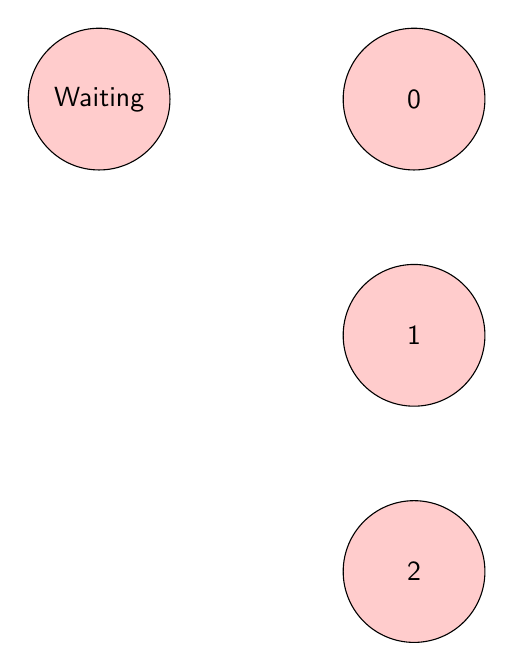
\begin{tikzpicture}[umlstate/.style={
    circle,
    draw,
    minimum size=1.8cm,
    fill=red!20,
    font=\sffamily
}]

\node[umlstate] (Waiting) at (-2,0) {Waiting};
\node[umlstate] (zero) at (2,0) {0};
\node[umlstate] (one) at (2,-3) {1};
\node[umlstate] (two) at (2,-6) {2};

\umltrans[arg=graspAt,pos=0.5]{Waiting}{zero}
\umltrans[arg=notifyEnd,pos=0.5]{zero}{one}
\umltrans[arg=notifyEnd,pos=0.5]{one}{two}
\umltrans[arg=notifyEnd,pos=1.5,arm1=3cm,geometry=-|-]{two}{zero}

\end{tikzpicture}
\end{center}
\end{figure}

Por lo tanto, el estado \textit{Waiting} no implementa \verb|notifyOrder|, mientras que los estados 0, 1 y 2 no implementan \verb|graspAt|. En cambio, \textit{Waiting} sí implementa \verb|graspAt|, el cual calcula los pasos y ejecuta el primero utilizando el iterador. Posteriormente, por cada \verb|notifyEnd| los subsistemas informan al \MainController que finalizaron la ejecución de la orden, y en cada notificación se transiciona a un nuevo estado. Una vez ejecutado \verb|graspAt|, se transiciona al estado 0; al recibir un \verb|notifyEnd| se pasa al estado 1, y de la misma forma hasta llegar al estado 2. Cuando se está en el estado 2 y se recibe un \verb|notifyEnd|, lo que ocurre es que se ejecuta un nuevo paso si aún quedan pasos en el iterador; en caso contrario, se transiciona nuevamente a \textit{Waiting}, dado que la secuencia de ejecución ha finalizado.

Está claro que, para poder sostener este comportamiento, los subsistemas deben responder a estas necesidades. Es decir, cada uno debe invocar el método \verb|notifyEnd| del \MainController como un \textit{callback} cuando realmente hayan terminado de ejecutar la orden, es decir, cuando alcanzan el \textit{set-point}. Los subsistemas son los encargados de determinar cuándo un paso se completó. En el caso de aquellos que requieren un seguimiento exhaustivo, al llegar al \textit{set-point} se transiciona del estado \textit{Moving} al estado \textit{Waiting}; en ese punto se puede incluir la llamada a \verb|notifyEnd|, como ocurre en el método \verb|moving| del módulo \Moving. En el caso del subsistema de la pinza, que no requiere seguimiento, la llamada puede agregarse inmediatamente después de aplicar el cambio en el módulo \Pinza.

\subsubsection*{Conclusión}

La solución propuesta mejora varios aspectos a la que utiliza como criterio de división la funcionalidad. Por un lado, se anticipa a cambios probables tales como los de la tabla \ref{tablaConclu}.

\begin{table}[H]
\centering
\caption{Anticipos al cambio del diseño propuesto para el brazo robótico.}
\label{tablaConclu}
\resizebox{\textwidth}{!}{%
\begin{tabular}{|p{3cm}|p{5cm}|p{8cm}|}
\hline
\textbf{Item de cambio}    & \textbf{Naturaleza del cambio}  & \textbf{Manejo del cambio}  \\ \hline
\textbf{Hardware}          &  
    - Agregar, quitar o modificar actuadores y sensores.
    
    - Cambios en la comunicación.
&  
Los subsistemas están desacoplados del control principal, permitiendo agregar, quitar o modificar componentes de manera independiente respetando las interfaces definidas.  
La modularización permite gestionar sensores, actuadores y comunicación por separado. La lógica de control puede modificarse fácilmente cambiando la implementación del módulo Algoritmo.
\\ \hline
\textbf{Lógica de control} &  
    - Cambios en decisiones de trabajo, como ejecución secuencial o criterios de avance.
&  
El comportamiento está encapsulado en módulos. La máquina de estados que controla la ejecución puede modificarse fácilmente agregando o editando estados en el iterador Steps.  
\\ \hline
\end{tabular}
}
\end{table}

Además, se fomenta la reutilización del código, permitiendo aplicar las soluciones existentes a distintos problemas. Cualquier modificación futura requerirá menos esfuerzo por parte de los desarrolladores, ya que el sistema será más fácil de comprender. La documentación también contribuye a esta facilidad de mantenimiento. Los cambios probables están encapsulados, por lo que el control de calidad se reduce a verificar módulos individuales y no secciones de código enteras.

% .tex extension is presumed
% \include{chapter2}
% \include{chapter3}
% \include{chapter4}


%%% Appendicies of thesis  %%%%%%%%%%%%%%%%%%%%%%%%%%%%%%%%%%%%%%%%%%%%%%%%%%%%%%%%%%%%%%%%%%%%%%%%

\appendix
% From mitthesis package
% Version: 1.01, 2023/07/04
% Documentation: https://ctan.org/pkg/mitthesis


\chapter{Patrones de diseño de Gamma}
\label{apendice}

En este apéndice se resumen los patrones de diseño de Gamma \cite{Gamma:1995:DPE:186897} utilizados en las soluciones a los problemas comunes. En el libro se encuentra una descripción completa de los mismos. Aquí solo se menciona la intención, aplicabilidad, participantes y estructura de cada patrón. El propósito es utilizar este apéndice a manera de complemento al entendimiento de cada aplicación de patrón.

\section{Adapter}

\subsection*{Intención}

Convierte la interfaz de una clase en otra interfaz que los clientes esperan, permitiendo que clases con interfaces incompatibles trabajen juntas. Es una solución para integrar clases existentes sin modificar su código original, asegurando que cumplan con los requisitos de una aplicación específica.

\subsection*{Aplicabilidad}

\begin{itemize}
\item Se desea usar una clase existente cuya interfaz no coincide con la requerida.
\item Se necesita crear una clase reutilizable que coopere con clases no relacionadas o no previstas inicialmente.
\item Se necesita adaptar varias subclases existentes sin modificar su interfaz de manera individual.
\end{itemize}


\subsection*{Participantes}

\begin{itemize}
\item \textbf{Objetivo}\\
Define la interfaz específica del dominio que el cliente utiliza.
\item \textbf{Clientes}\\
Colabora con objetos que cumplen con la interfaz del \textbf{Objetivo}.
\item \textbf{Adaptable}\\
Define una interfaz existente que necesita ser adaptada.
\item \textbf{Adaptador}\\
Adapta la interfaz del \textbf{Adaptable} para que cumpla con la interfaz del \textbf{Objetivo}.
\end{itemize}

\subsection*{Estructura}

\begin{figure}[h]
\caption{Estructura patrón \textbf{Adapter}}
\begin{center}
\begin{tikzpicture}\sf
\umlsimpleclass[x=-4.5,y=1]{Cliente}

\umlclass[x=0,y=1,type=abstract]{Objetivo}
{}
{
\umlvirt{peticion()}
}
\umlclass[below=1.5cm of Objetivo]{Adaptador}
{}
{
peticion()
}
\umlclass[x=6]{Adaptable}
{}
{
peticionConcreta()
}
umluniassoc
\umlinherit[geometry=|-|]{Adaptador}{Objetivo}
\umluniassoc[]{Cliente}{Objetivo}
\umluniassoc[geometry=-|-]{Adaptador}{Adaptable}
\end{tikzpicture}
\end{center}
\end{figure}


\section{Command}


\subsection*{Intención}

El patrón encapsula una solicitud como un módulo, permitiendo parametrizar clientes con diferentes solicitudes, encolar o registrar solicitudes, y admitir operaciones reversibles. Este enfoque facilita la creación de sistemas flexibles y extensibles que manejan comandos de manera uniforme.

\subsection*{Aplicabilidad}

\begin{itemize}
\item Parametrizar objetos con una acción a realizar. Esta parametrización puede expresarse en un lenguaje procedimental mediante una función de \gls{callback}, es decir, una función registrada para ser llamada posteriormente. Los comandos representan una solución orientada a objetos que reemplaza los \glspl{callback}.

\item Especificar, encolar y ejecutar solicitudes en diferentes momentos. Un módulo \textbf{Command} puede tener una vida útil independiente de la solicitud original. Si el receptor de una solicitud puede representarse de forma independiente del espacio de direcciones, puedes transferir un objeto \textbf{Command} a otro proceso y ejecutar la solicitud allí.

\item Soportar la funcionalidad de deshacer (``undo''). El método \textbf{Execute} del \textbf{Command} puede almacenar el estado necesario para revertir sus efectos. La interfaz del \textbf{Command} debe incluir una operación \textbf{Unexecute} para revertir los efectos de una ejecución previa. Los comandos ejecutados se almacenan en una lista de historial, lo que permite deshacer y rehacer a múltiples niveles navegando hacia adelante y hacia atrás en la lista mientras se llaman a \textbf{Unexecute} y \textbf{Execute}.

\item Registrar cambios para que puedan reaplicarse en caso de una falla del sistema. Al ampliar la interfaz del \textbf{Command} con operaciones de carga y almacenamiento, puedes mantener un registro persistente de los cambios. Recuperar un sistema tras una falla implica recargar los comandos registrados desde el disco y reejecutarlos mediante la operación \textbf{Execute}.

\item Estructurar un sistema en torno a operaciones de alto nivel basadas en operaciones primitivas. Esta estructura es común en sistemas de información que admiten transacciones. Una transacción encapsula un conjunto de cambios a los datos. El patrón \textbf{Command} proporciona una forma de modelar transacciones, ya que los comandos tienen una interfaz común, lo que permite invocar todas las transacciones de la misma manera. Además, el patrón facilita la extensión del sistema con nuevas transacciones.
\end{itemize}


\subsection*{Participantes}

\begin{itemize}
\item \textbf{Orden}\\
Declara una interfaz para ejecutar una operación.

\item \textbf{OrdenConcreta}\\
Define una asociación entre un módulo receptor (Receiver) y una acción.
Implementa el método Execute invocando las operaciones correspondientes en el receptor.

\item \textbf{Cliente}\\
Utiliza OrdenConcreta y configura su receptor.

\item \textbf{Invocador}\\
Solicita al comando que lleve a cabo la solicitud.

\item \textbf{Receptor}\\
Conoce cómo realizar las operaciones asociadas con la ejecución de una solicitud. Cualquier clase puede actuar como un receptor.
\end{itemize}


\subsection*{Estructura}

\begin{figure}[h]
\caption{Estructura patrón \textbf{Command}}
\begin{center}
\begin{tikzpicture}\sf
\umlsimpleclass[]{Invocador}
\umlclass[right=2cm of Invocador,type=abstract]{Orden}
{}
{
\umlvirt{ejecutar()}
}
\umlclass[below=2cm of Invocador]{Receptor}
{}
{
acción
}

\umlclass[below=1.45cm of Orden]{OrdenConcreta}
{}
{
ejecutar()
}

\umluniassoc{OrdenConcreta}{Receptor}
\umlinherit{OrdenConcreta}{Orden}
\umluniaggreg{Invocador}{Orden}

\end{tikzpicture}
\end{center}
\end{figure}


\section{State}

\label{anexoState}

\subsection*{Intención}

Permitir que un módulo altere su comportamiento cuando su estado interno cambia. El módulo parecerá cambiar de clase.

\subsection*{Aplicabilidad}

\begin{itemize}
\item El comportamiento de un objeto depende de su estado, y debe cambiar su comportamiento en tiempo de ejecución según ese estado.
\item Las operaciones suelen tener declaraciones condicionales grandes y complejas que dependen del estado del módulo. Este estado generalmente está representado por una o más constantes enumeradas. Frecuentemente, varias operaciones comparten la misma estructura condicional. El patrón separa cada rama de la estructura condicional en una clase independiente. Esto permite tratar el estado del módulo como un módulo por derecho propio, que puede variar independientemente de otros módulos.
\end{itemize}

\subsection*{Participantes}

\begin{itemize}
\item \textbf{Contexto}\\
Define la interfaz de interés para los clientes. Mantiene una instancia de una subclase de EstadoConcreto que define el estado actual.

\item \textbf{Estado}\\
Define una interfaz para encapsular el comportamiento asociado con un estado particular del contexto.

\item \textbf{EstadoConcreto}\\
Cada subclase implementa un comportamiento asociado con un estado del contexto.
\end{itemize}


\subsection*{Estructura}

\begin{figure}[h]
\caption{Estructura patrón \textbf{State}}
\begin{center}
\begin{tikzpicture}\sf
\umlclass[]{Contexto}
{}
{
peticion()
}
\umlnote[below=1cm of Contexto]{Contexto}
{
estado.manejar()
}

\umlclass[right=7cm of Context,type=abstract]{Estado}
{}
{
\umlvirt{manejar()}
}
\umlclass[below left=1.5cm and -0.5cm of Estado]{EstadoConcretoA}
{}
{
manejar()
}
\umlclass[below right=1.5cm and -0.5cm of Estado]{EstadoConcretoB}
{}
{
manejar()
}

\umlinherit[geometry=|-|]{EstadoConcretoB}{Estado}
\umlinherit[geometry=|-|]{EstadoConcretoA}{Estado}
\umluniaggreg[]{Contexto}{Estado}

\end{tikzpicture}
\end{center}
\end{figure}

\section{Mediator}
\label{anexoMediator}

\subsection*{Intención}
Define un modulo que encapsula cómo interactúa un conjunto de módulos. Fomenta un acoplamiento débil al evitar que los objetos se refieran explícitamente entre sí, y permite variar sus interacciones de manera independiente.

\subsection*{Aplicabilidad}
\begin{itemize}
\item Un conjunto de módulos se comunica de maneras bien definidas pero complejas. Las interdependencias resultantes son desestructuradas y difíciles de comprender.

\item Reutilizar un módulo resulta complicado porque este se refiere y se comunica con muchos otros módulos.

\item Un comportamiento distribuido entre varios módulos debería ser personalizable sin requerir una gran cantidad de subclases.
\end{itemize}

\subsection*{Participantes}

\begin{itemize}
\item \textbf{Mediador} Define una interfaz para comunicarse con los módulos Colega.
\item \textbf{MediadorConcreto} Implementa un comportamiento cooperativo coordinando los módulos Colega. Conoce y mantiene a sus colegas.
\item \textbf{Colega} Conoce a su objeto Mediator y se comunica con se siempre que, de otra forma, se habría comunicado con otro Colega.
\end{itemize}

\subsection*{Estructura}

\begin{figure}[h]
\caption{Estructura patrón \textbf{Mediator}}
\begin{center}
\begin{tikzpicture}\sf
\umlsimpleclass[type=abstract]{Mediador}

\umlsimpleclass[below=1.5cm of Mediador]{MediadorConcreto}

\umlsimpleclass[right=7cm of Mediador,type=abstract]{Colega}

\umlsimpleclass[below left=1.5cm and -0.5cm of Colega]{ColegaConcretoA}

\umlsimpleclass[below right=1.5cm and -0.5cm of Colega]{ColegaConcretoB}

\umlinherit[geometry=|-|]{ColegaConcretoB}{Colega}
\umlinherit[geometry=|-|]{ColegaConcretoA}{Colega}
\umlinherit[]{MediadorConcreto}{Mediador}
\umluniassoc[]{Colega}{Mediador}
\umluniassoc[]{MediadorConcreto}{ColegaConcretoA}
\umluniassoc[geometry=|-|,arm1=-0.7cm,anchor1=-30,anchor2=-150]{MediadorConcreto}{ColegaConcretoB}



\end{tikzpicture}
\end{center}
\end{figure}

\section{Decorator}
\label{anexoDecorator}

\subsection*{Intención}
Agregar responsabilidades adicionales a un objeto de manera dinámica. Los decoradores ofrecen una alternativa flexible a la herencia para extender la funcionalidad.

\subsection*{Aplicabilidad}
\begin{itemize}
\item Agregar responsabilidades a objetos individuales de manera dinámica y transparente, es decir, sin afectar a otros objetos.
\item Para responsabilidades que pueden ser eliminadas.
\item Cuando la extensión mediante herencia es impracticable. A veces, es posible tener una gran cantidad de extensiones independientes, lo que produciría una explosión de subclases para admitir cada combinación. O bien, la definición de una clase puede estar oculta o no estar disponible para la subclase.
\end{itemize}

\subsection*{Participantes}
\begin{itemize}
\item \textbf{Componente} Define la interfaz para módulos a los que se les pueden agregar responsabilidades de manera dinámica.
\item \textbf{ComponenteConcreto} Define un módulo al que se le pueden adjuntar responsabilidades adicionales.
\item \textbf{Decorador} Mantiene una referencia a un módulo \textbf{Componente} y define una interfaz que se ajusta a la interfaz del \textbf{Componente}.
\item \textbf{DecoradorConcreto} Agrega responsabilidades al componente.
\end{itemize}


\subsection*{Estructura}

\begin{figure}[h]
\caption{Estructura patrón \textbf{Decorator}}
\begin{center}
\begin{tikzpicture}\sf
\umlclass[type=abstract]{Componente}{}
{
\umlvirt{operacion()}
}

\umlclass[below left=2cm and -1cm of Componente]{ComponenteConcreto}{}
{
operacion()
}

\umlclass[below right=2cm and -1cm of Componente,type=abstract]{Decorador}{}
{
\umlvirt{operacion()}
}

\umlclass[below right=2cm and -1cm of Decorador]{DecoradorConcretoA}{}
{
operacion() \\
comportamientoAñadido()
}

\umlclass[below left=2cm and -1cm of Decorador]{DecoradorConcretoB}
{
estadoAñadido
}
{
operacion() \\
}

\umlnote[right=4cm of Decorador,width=4.5cm]{Decorador}{
operacion \{\\
\ \ componente.operacion()\\
\}
}

\umlinherit[geometry=|-|]{ComponenteConcreto}{Componente}
\umlinherit[geometry=|-|]{Decorador}{Componente}
\umlinherit[geometry=|-|]{DecoradorConcretoA}{Decorador}
\umlinherit[geometry=|-|,arm1=2.04cm]{DecoradorConcretoB}{Decorador}
\umluniaggreg[geometry=-|-,arm1=3cm,anchor1=20,arg1=componente,pos1=0.5]{Decorador}{Componente}



\end{tikzpicture}
\end{center}
\end{figure}




\section{Proxy}
\label{patronProxy}

\subsection*{Intención}
Proporcionar un sustituto o marcador de posición para otro objeto con el fin de controlar el acceso a este.

\subsection*{Aplicabilidad}

El patrón Proxy es aplicable siempre que se necesite una referencia más versátil o sofisticada a un objeto que un simple puntero. Estas son varias situaciones comunes en las que se puede aplicar el patrón:

\begin{enumerate}
\item Proxy Remoto:

Proporciona un representante local para una instancia en un espacio de direcciones diferente.

\item Proxy Virtual:

Crea instancias costosas bajo demanda.

\item Proxy de Protección:

Controla el acceso a la instancia original.
Es útil cuando las instancias necesitan diferentes derechos de acceso.

\item Referencia Inteligente:

Es un reemplazo para un puntero básico que realiza acciones adicionales cuando se accede a un objeto.
Usos típicos incluyen:
\begin{itemize}
\item Contar el número de referencias a la instancia real para que pueda ser liberado automáticamente cuando no queden más referencias (también llamado punteros inteligentes).
\item Cargar una instancia persistente en memoria cuando se referencia por primera vez.
\item Verificar que la instancia real esté bloqueado antes de acceder a ella, para asegurar que ningún otra instancia pueda modificarlo.
\item 
Este patrón ofrece flexibilidad, seguridad y eficiencia en la gestión de interacciones entre instancias.
\end{itemize}

\end{enumerate}


\subsection*{Participantes}

\begin{itemize}
\item \textbf{Proxy} Mantiene una referencia que permite al proxy acceder al sujeto real. El Proxy puede referirse a un \textbf{Sujuteo} si las interfaces de \textbf{SujetoReal} y \textbf{Sujeto} son las mismas.
Proporciona una interfaz idéntica a la de \textbf{Sujeto}, de manera que un proxy puede ser sustituido por el sujeto real.
Controla el acceso al sujeto real y puede ser responsable de crearlo y eliminarlo.

\item \textbf{Sujeto} Define la interfaz común para \textbf{SujetoReal} y \textbf{Proxy}, de modo que un \textbf{Proxy} se pueda usar en cualquier lugar donde se espere un \textbf{SujetoReal}.

\item \textbf{RealSubject} Define el objeto real que el proxy representa.

\end{itemize}


\subsection*{Estructura}


\begin{figure}[h]
\caption{Estructura patrón \textbf{Proxy}}
\begin{center}
\begin{tikzpicture}\sf
\umlclass[type=abstract]{Sujeto}{}
{
\umlvirt{peticion()}
}

\umlclass[below left=1.5cm and -0.5cm of Sujeto]{SujetoReal}{}
{
peticion() \\
...
}

\umlclass[below right=1.5cm and -0.5cm of Sujeto]{Proxy}{}
{
peticion() \\
...
}

\umlnote[right=2cm of Proxy,width=4cm]{Proxy}{
...\\
sujetoReal.peticion()\\
...}

\umlinherit[geometry=|-|]{SujetoReal}{Sujeto}
\umlinherit[geometry=|-|]{Proxy}{Sujeto}
\umluniassoc[]{Proxy}{SujetoReal}



\end{tikzpicture}
\end{center}
\end{figure}




\section{Iterator}
\label{patronIterator}

\subsection*{Intención}
Proporcionar un modo de acceder secuencialmente a elementos de un módulo sin exponer su representación interna.

\subsection*{Aplicabilidad}

Úsese el patrón Iterador:
\begin{itemize}
\item Para acceder al contenido de un módulo agregado sin exponer su representación interna.
\item Para permitir varios recorridos sobre objetos agregados.
\item Para proporcionar una interfaz uniforme para recorrer diferentes estructuras agregadas (es decir, para permitir la iteración polimórfica).

\end{itemize}


\subsection*{Participantes}

\begin{itemize}
\item \textbf{Iterador} Define una interfaz para recorrer los elementos y acceder a ellos.

\item \textbf{IteradorConcreto} Implementa la interfaz de \textbf{Iterator}.

\item \textbf{Agregado} Define una interfaz para crear una instancia de \textbf{Iterator}.

\item \textbf{AgregadoConcreto} Implementa la interaz de Agregado.

\end{itemize}


\subsection*{Estructura}


\begin{figure}[h]
\caption{Estructura patrón \textbf{Iterador}}
\begin{center}
\begin{tikzpicture}\sf
\umlsimpleclass{Cliente}

\umlclass[left=1.5cm of Cliente]{Agregado}{}
{
crearIterator() \\
}

\umlclass[below=2cm of Agregado]{AgregadoConcreto}{}
{
crearIterator() \\
}


\umlclass[right=1.5cm of Cliente]{Iterador}{}
{
primero() \\
siguiente() \\
haTerminado() \\
elementoActual() \\
}

\umlclass[below right=2cm and 4.83cm of Agregado]{IteradorConcreto}{}
{
primero() \\
siguiente() \\
haTerminado() \\
elementoActual() \\
}

\umlnote[below=1cm of AgregadoConcreto,withd=4cm]{AgregadoConcreto}{
return new IteradorConcreto()
}

\umlinherit{IteradorConcreto}{Iterador}
\umlinherit{AgregadoConcreto}{Agregado}
\umluniassoc[]{Cliente}{Iterador}
\umluniassoc[]{Cliente}{Agregado}


\end{tikzpicture}
\end{center}
\end{figure}











%%% Bibliography (biblatex)  %%%%%%%%%%%%%%%%%%%%%%%%%%%%%%%%%%%%%%%%%%%%%%%%%%%%%%%%%%%%%%%%%%%%%%

\defbibheading{bibintoc}{\chapter*{#1}\addcontentsline{toc}{backmatter}{\refname}} 
% this sets the title of contents name for bibliography to \refname (= References)
% change "backmatter" to "chapter" if you prefer a bold face entry in the table of contents

\printbibliography[title={\refname},heading=bibintoc]

% biblatex also supports chapter-by-chapter bibliography, https://tex.stackexchange.com/a/296502/119566
% see the biblatex manual, section 3.14.3


%%%% Option for natbib %%%%%%%%%%%%%

%%   use an appropriate style (.bst) and your own .bib file[s]

%\bibliographystyle{plainnat}
%\bibliography{mitthesis-sample.bib}

\end{document} 
 